\documentclass[12pt]{book}
% !TEX root = hazy3.tex
%\includeonly{isoseq}
%\includeonly{hydroiso}
%\includeonly{helikeiso}
%\includeonly{molecules}
%\includeonly{dheavy}
%\includeonly{dtherm}
%\includeonly{dgrain}
%\includeonly{dother}
%\includeonly{refer}

\usepackage{graphicx,rotate,url,mathptmx,lscape,times,framed,color}

% include natbib for bibtex, options are
% round use (2008) instead of [2008] for year
\usepackage[round]{natbib}

% cross references across documents
\usepackage{xr-hyper}

%\begin{comment}
%This is my comment.
%Note that it can span multiple lines.
%This is very useful.
%\end{comment}
\usepackage{verbatim} 

% allow hyperlinks
\usepackage{hyperref}
\hypersetup{
    bookmarks=true,         % show bookmarks bar?
    unicode=false,          % non-Latin characters in Acrobat's bookmarks
    pdftoolbar=true,        % show Acrobat's toolbar?
    pdfmenubar=true,        % show Acrobat's menu?
    pdffitwindow=true,      % page fit to window when opened
    pdftitle={My title},    % title
    pdfauthor={Author},     % author
    pdfsubject={Subject},   % subject of the document
    pdfnewwindow=true,      % links in new window
    pdfkeywords={keywords}, % list of keywords
    colorlinks=true,        % false: boxed links; true: colored links
    linkcolor=blue,         % color of internal links, def red
    citecolor=blue,         % color of links to bibliography, def green
    filecolor=blue,         % color of file links, def magenta
    urlcolor=blue           % color of external links, def cyan
}

% geometry package controls page layout
\usepackage[letterpaper,
left=2.5cm,right=2.5cm,
top=2.5cm,bottom=2.5cm]{geometry}
\oddsidemargin=+0.7cm
\evensidemargin=-0.7cm
\pagestyle{headings}

% journal name macros used by ADS
\usepackage{../common/aas_macros_v61}

% Include list of figures and references in contents lists
\usepackage[nottoc]{tocbibind}

% makes it easy to include all or part of a PDF document 
% inside a LaTeX document
\usepackage{pdfpages}

% allow external files to be included verbatim
\usepackage{moreverb}

% allow tables to wrap over pages
\usepackage{longtable}


% set the default tabsize
\def\verbatimtabsize{4\relax}

% following are to pick up .aux files for cross references
% with package xr to other volumes of Hazy
% hazy 1
\externaldocument[Hazy1-]{../hazy1/intro}[hazy1.pdf]
\externaldocument[Hazy1-]{../hazy1/define}[hazy1.pdf]
\externaldocument[Hazy1-]{../hazy1/cmdintro}[hazy1.pdf]
\externaldocument[Hazy1-]{../hazy1/cont-def}[hazy1.pdf]
\externaldocument[Hazy1-]{../hazy1/cont-lum}[hazy1.pdf]
\externaldocument[Hazy1-]{../hazy1/cont-shp}[hazy1.pdf]
\externaldocument[Hazy1-]{../hazy1/compos}[hazy1.pdf]
\externaldocument[Hazy1-]{../hazy1/density}[hazy1.pdf]
\externaldocument[Hazy1-]{../hazy1/geometry}[hazy1.pdf]
\externaldocument[Hazy1-]{../hazy1/optdepth}[hazy1.pdf]
\externaldocument[Hazy1-]{../hazy1/therm}[hazy1.pdf]
\externaldocument[Hazy1-]{../hazy1/dynamics-time}[hazy1.pdf]
\externaldocument[Hazy1-]{../hazy1/stopping}[hazy1.pdf]
\externaldocument[Hazy1-]{../hazy1/conout}[hazy1.pdf]
\externaldocument[Hazy1-]{../hazy1/optimize}[hazy1.pdf]
\externaldocument[Hazy1-]{../hazy1/grid}[hazy1.pdf]
\externaldocument[Hazy1-]{../hazy1/miscell}[hazy1.pdf]
\externaldocument[Hazy1-]{../hazy1/latex_style}[hazy1.pdf]

% hazy2
\externaldocument[Hazy2-]{../hazy2/limits}[hazy2.pdf]
\externaldocument[Hazy2-]{../hazy2/coninter}[hazy2.pdf]
\externaldocument[Hazy2-]{../hazy2/lineatomparam}[hazy2.pdf]
\externaldocument[Hazy2-]{../hazy2/linedetl}[hazy2.pdf]
\externaldocument[Hazy2-]{../hazy2/CloudyStandaloneProgram}[hazy2.pdf]
\externaldocument[Hazy2-]{../hazy2/sub}[hazy2.pdf]
\externaldocument[Hazy2-]{../hazy2/output}[hazy2.pdf]
\externaldocument[Hazy2-]{../hazy2/observed}[hazy2.pdf]
\externaldocument[Hazy2-]{../hazy2/lines}[hazy2.pdf]
\externaldocument[Hazy2-]{../hazy2/problems}[hazy2.pdf]
\externaldocument[Hazy2-]{../hazy2/odetail}[hazy2.pdf]
\externaldocument[Hazy2-]{../hazy2/sources}[hazy2.pdf]
\externaldocument[Hazy2-]{../hazy2/glossary}[hazy2.pdf]
\externaldocument[Hazy2-]{../hazy2/conversion}[hazy2.pdf]
\externaldocument[Hazy2-]{../hazy2/TestSuite}[hazy2.pdf]

% hazy 3
\externaldocument[Hazy3-]{../hazy3/isoseq}[hazy3.pdf]
\externaldocument[Hazy3-]{../hazy3/hydroiso}[hazy3.pdf]
\externaldocument[Hazy3-]{../hazy3/helikeiso}[hazy3.pdf]
\externaldocument[Hazy3-]{../hazy3/molecules}[hazy3.pdf]
\externaldocument[Hazy3-]{../hazy3/dheavy}[hazy3.pdf]
\externaldocument[Hazy3-]{../hazy3/dtherm}[hazy3.pdf]
\externaldocument[Hazy3-]{../hazy3/dgrain}[hazy3.pdf]
\externaldocument[Hazy3-]{../hazy3/dother}[hazy3.pdf]

% set paragraph styles
\raggedright
\setlength{\parindent}{4mm}
% background color for shaded boxes
\definecolor{shadecolor}{gray}{0.9}

% Customize contents details from book.cls
\makeatletter

\renewcommand*\l@section{\@dottedtocline{1}{1.5em}{3.1em}}
\renewcommand*\l@subsection{\@dottedtocline{2}{4.6em}{4.1em}}
\renewcommand*\l@subsubsection{\@dottedtocline{3}{8.7em}{5.1em}}
\renewcommand*\l@paragraph{\@dottedtocline{4}{10em}{6em}}
\renewcommand*\l@subparagraph{\@dottedtocline{5}{12em}{7em}}
\renewcommand*\l@figure{\@dottedtocline{1}{1.5em}{3.3em}}

% extract name of target of reference (e.g. chapter titles)
\long\def\@thirdoffive#1#2#3#4#5{#3}%
\def\refname#1{\expandafter\@setref\csname r@#1\endcsname\@thirdoffive{#1}}

% create ruler underneath page header
\advance\headheight1.2pt
\def\@oddhead{\vbox{\parindent=0pt%
\setbox0=\hbox to\textwidth{{\slshape\rightmark}\hfil\thepage}%
\dimen0=4.5pt \advance\dimen0 by-\dp0 \box0\kern\dimen0\hrule}}
\def\@evenhead{\vbox{\parindent=0pt%
\setbox0=\hbox to\textwidth{\thepage\hfil\slshape\leftmark}%
\dimen0=4.5pt \advance\dimen0 by-\dp0 \box0\kern\dimen0\hrule}}

% modify font size for verbatim environment
\newcommand{\setverbatimfontsize}[1]{\renewcommand*\verbatim@font{#1\ttfamily}}
\renewcommand*\verbatim@font{\footnotesize\ttfamily}

% Change title of bibliography
\renewcommand\bibname{REFERENCES}
\renewcommand\contentsname{CONTENTS}
\renewcommand\listfigurename{LIST OF FIGURES}
\renewcommand\listtablename{LIST OF TABLES}
% tweak bibliograpy environment to be more like old Hazy
\def\thebibliography#1{%
\bibsection
\@mkboth{\MakeUppercase\bibname}{\MakeUppercase\bibname}%
\list{}{\setlength\labelwidth{2.5em}\leftmargin\labelwidth
\setlength\parsep{0pt}\setlength\itemsep{0.7mm plus1pt}
\setlength{\itemindent}{-\leftmargin}
\small}
\def\newblock{\hskip .11em plus .33em minus -.07em}
\sloppy
\sfcode`\.=1000\relax}
\def\endthebibliography{\endlist}


\setcounter{tocdepth}{4}

\makeatother
% End of contents customization

% 20 06 24, copied from  aastex63.cls

%% need this change so that it works correctly in tables:
{\catcode`\$=\active
\gdef\nodata{ ~$\cdots$~ }}% 

\newcommand\diameter{\ooalign{\hfil/\hfil\crcr\mathhexbox20D}}% 
\newcommand\degr{\arcdeg}% 
\newcommand\Sun{\sun}% 
\newcommand\Sol{\sun}% 
\newcommand\sun{\odot}% 
\newcommand\Mercury{\astro{\char1}}% Mercury symbol, "1" 
\newcommand\Venus{\astro{\char2}}% Venus symbol, "2" 
\newcommand\Earth{\earth}% 
\newcommand\Terra{\earth}% 
\newcommand\earth{\oplus}% 
\newcommand\Mars{\astro{\char4}}% Mars symbol, "4" 
\newcommand\Jupiter{\astro{\char5}}% Jupiter symbol, "5" 
\newcommand\Saturn{\astro{\char6}}% Saturn symbol, "6" 
\newcommand\Uranus{\astro{\char7}}% Uranus symbol, "7" 
\newcommand\Neptune{\astro{\char8}}% Neptune symbol, "8" 
\newcommand\Pluto{\astro{\char9}}% Pluo symbol, "9" 
\newcommand\Moon{\astro{\char10}}% Moon symbol, "M" 
\newcommand\Luna{\Moon}% 
\newcommand\Aries{\astro{\char11}}% 
\newcommand\VEq{\Aries}% vernal equinox (Aries) 
\newcommand\Taurus{\astro{\char12}}% 
\newcommand\Gemini{\astro{\char13}}% 
\newcommand\Cancer{\astro{\char14}}% 
\newcommand\Leo{\astro{\char15}}% 
\newcommand\Virgo{\astro{\char16}}% 
\newcommand\Libra{\astro{\char17}}% 
\newcommand\AEq{\Libra}% autumnal equinox (Libra) 
\newcommand\Scorpius{\astro{\char18}}% 
\newcommand\Sagittarius{\astro{\char19}}% 
\newcommand\Capricornus{\astro{\char20}}% 
\newcommand\Aquarius{\astro{\char21}}% 
\newcommand\Pisces{\astro{\char22}}% 
 

% some names we use
\newcommand{\Cloudy}{\textsc{Cloudy}}
\newcommand{\Hazy}{\textsc{Hazy}}
\newcommand{\cdCommand}[1]{\textbf{#1}}
\newcommand{\cdVariable}[1]{\emph{#1}}
\newcommand{\cdSectionTitle}[1]{\emph{#1}}
\newcommand{\cdFilename}[1]{\texttt{#1}}
\newcommand{\cdRoutine}[1]{\emph{#1}}
\newcommand{\cdTerm}[1]{\textbf{\emph{#1}}}
\newcommand{\cdMono}[1]{\texttt{#1}}
\newcommand{\fixit}[1]{\textbf{FIXIT: #1}}
\font\manual=manfnt at 7pt \def\dbend{\hbox{\raise0.9ex\hbox{\manual\char127\hspace{0.6em}}}}
\newcommand{\experimental}{\texorpdfstring{\dbend}{??}}

% or symbol provided by Will H
\newcommand\OR{\texorpdfstring{\ensuremath{\vert}}{|}}

% Matt's 1.23\e{-2} 
\providecommand{\e}[1]{\ensuremath{\times 10^{#1}}}


% \ion from Will, replace AAS version
\newcommand\Ion[2]{\ensuremath{\mathrm{#1\,\scriptstyle #2}}}

% macro sometimes found in ADS bibtex entries
\newcommand{\mdash}{---} 

% ion is in the aas style
\newcounter{INTERNALionstage}
\providecommand{\ion}[2]{% replace the aastex version
  \setcounter{INTERNALionstage}{#2}%
  \Ion{#1}{\Roman{INTERNALionstage}}}

\providecommand{\red}[1]{{\color{red}#1}}

% Will's todo and done macros
%\newcommand\TODO[1]{\textbf{\boldmath [#1]}}
\newcommand{\TODO}[1]{\textcolor{red}{{\textbf{\boldmath [#1]}}}}
\newcommand\DONE[1]{{\color{green!50!gray} \textbf{DONE}} {\color{white!80!black!80!green} #1}}

\newcommand{\Av}{A$_{\rm V}$}

\def\gtsim{\mathrel{\hbox{\rlap{\hbox{\lower4pt\hbox{$\sim$}}}\hbox{$>$}}}}
\def\lesssim{\mathrel{\hbox{\rlap{\hbox{\lower4pt\hbox{$\sim$}}}\hbox{$<$}}}}
\def\Msunpyr{M$_{\odot}\,$yr$^{-1}$}
\def\Msun{M$_{\odot}$}
%       Based on PATs UNITS.TEX with some additions
%
%       Simple units
%
\def\A{{\rm\thinspace \AA}}
\def\cm{{\rm\thinspace cm}}
\def\as{{\rm\thinspace arcsec}}
\def\erg{{\rm\thinspace erg}}
\def\eV{{\rm\thinspace eV}}
\def\g{{\rm\thinspace g}}
\def\ga{{\rm\thinspace gauss}}
\def\hr{{\rm\thinspace hr}}
\def\Hz{{\rm\thinspace Hz}}
\def\K{{\rm\thinspace K}}
\def\keV{{\rm\thinspace keV}}
\def\km{{\rm\thinspace km}}
\def\kpc{{\rm\thinspace kpc}}
\def\Lsun{\mbox{$\rm\thinspace L_{\odot}$}}
\def\m{{\rm\thinspace m}}
\def\MeV{{\rm\thinspace MeV}}
\def\mJy{{\rm\thinspace mJy}}
\def\micron{\hbox{$\mu$m}}
\def\Mpc{{\rm\thinspace Mpc}}
\def\Msun{\mbox{$\rm\thinspace M_{\odot}$}}
\def\nm{{\rm\thinspace nm}}
\def\pc{{\rm\thinspace pc}}
\def\ps{{\rm\thinspace s^{-1}}}
\def\pcc{{\rm\thinspace cm^{-3}}}
\def\Ryd{{\rm\thinspace Ryd}}
\def\s{{\rm\thinspace s}}
\def\sr{{\rm\thinspace sr}}
\def\W{{\rm\thinspace W}}
\def\yr{{\rm\thinspace yr}}
%
%       Compound units
%
\def\keVscm{\mbox{$\keV\cm^{2}\,$}}
\def\cmps{\mbox{$\cm\s^{-1}\,$}}
\def\cmpss{\mbox{$\cm\s^{-2}\,$}}
\def\ccmps{\mbox{$\cm^{3}\s^{-1}\,$}}
\def\ergpccmps{\mbox{$\erg\cm^{-3}\s^{-1}\,$}}
\def\ergpg{\mbox{$\erg\g^{-1}\,$}}
\def\ergpscm{\mbox{$\erg\cm^{-2}\,$}}
\def\ergpscmps{\mbox{$\erg\cm^{-2}\s^{-1}\,$}}
\def\ergpscmpspsas{\mbox{$\erg\cm^{-2}\s^{-1}\as^{-2}\,$}}
\def\ergpscmpspa{\mbox{$\erg\cm^{-2}\s^{-1}\A^{-1}\,$}}
\def\ergps{\mbox{$\erg\s^{-1}\,$}}
\def\gpcm{\mbox{$\g\cm^{-3}\,$}}
\def\gpcmps{\mbox{$\g\cm^{-3}\s^{-1}\,$}}
\def\gps{\mbox{$\g\s^{-1}\,$}}
\def\uJy{\mbox{$\mu${\rm Jy}}}
\def\kmps{\mbox{$\km\ps\,$}}
\def\kmpspMpc{\mbox{$\kmps\Mpc^{-1}\,$}}
\def\Lsunppc{\mbox{$\Lsun\pc^{-3}\,$}}
\def\Msunpc{\mbox{$\Msun\pc^{-3}\,$}}
\def\Msunpkpc{\mbox{$\Msun\kpc^{-1}\,$}}
\def\Msunppc{\mbox{$\Msun\pc^{-3}\,$}}
\def\Msunppcpyr{\mbox{$\Msun\pc^{-3}\yr^{-1}\,$}}
\def\Msunpyr{\mbox{$\Msun\yr^{-1}\,$}}
\def\Msunpyrpkpc{\mbox{$\Msun\yr^{-1}\kpc^{-1}\,$}}
\def\ps{\mbox{$\s^{-1}\,$}}
\def\pscm{\mbox{$\cm^{-2}\,$}}
\def\psm{\mbox{$\m^{-2}\,$}}
\def\pccm{\mbox{$\cm^{-3}\,$}}
\def\pscm{\mbox{$\cm^{-2}\,$}}
\def\pscmps{\mbox{$\cm^{-2}\, \s^{-1}\,$}}
\def\pcm{\mbox{$\m^{-3}\,$}}
\def\pccmK{\mbox{$\cm^{-3}\K$}}
\def\pcmK{\mbox{$\m^{-3}\K$}}
\def\pressure{\mbox{$\g\, \cm^{-1}\, \s^{-2}\,$}}
\def\pyr{\mbox{$\yr^{-1}\,$}}
\def\pyrppc{\mbox{$\yr^{-1}\pc^{-1}\,$}}
\def\scm{\mbox{$\cm^{2}\,$}}
\def\Wpsm{\mbox{$\W\psm\,$}}
\def\Wpscm{\mbox{$\W\pscm\,$}}
\def\WHz{\mbox{$\W\Hz\,$}}
%
% spectral lines
%
\def\la{\mbox{{\rm L}$\alpha$}}
\def\pa{\mbox{{\rm P}$\alpha$}}
\def\ha{\mbox{{\rm H}$\alpha$}}
\def\hb{\mbox{{\rm H}$\beta$}}
\def\hi{\mbox{{\rm H~{\sc i}}}}
\def\hii{\mbox{{\rm H~{\sc ii}}}}
\def\hei{\mbox{{\rm He~{\sc i}}}}
\def\heii{\mbox{{\rm He~{\sc ii}}}}
\def\ci{\mbox{{\rm C~{\sc i}}}}
\def\cii{\mbox{{\rm C~{\sc ii}}}}
\def\ciii{\mbox{{\rm C~{\sc iii}}}}
\def\civ{\mbox{{\rm C~{\sc iv}}}}
\def\ni{\mbox{{\rm N~{\sc i}}}}
\def\nii{\mbox{{\rm N~{\sc ii}}}}
\def\oi{\mbox{{\rm O~{\sc i}}}}
\def\oii{\mbox{{\rm O~{\sc ii}}}}
\def\oiii{\mbox{{\rm O~{\sc iii}}}}
\def\neii{\mbox{{\rm Ne~{\sc ii}}}}
\def\neiii{\mbox{{\rm Ne~{\sc iii}}}}
\def\nev{\mbox{{\rm Ne~{\sc v}}}}
\def\mgii{\mbox{{\rm Mg~{\sc ii}}}}
\def\cliii{\mbox{{\rm Cl~{\sc iii}}}}
\def\sii{\mbox{{\rm S~{\sc ii}}}}
\def\siii{\mbox{{\rm S~{\sc iii}}}}
\def\ariii{\mbox{{\rm Ar~{\sc iii}}}}
\def\caii{\mbox{{\rm Ca~{\sc ii}}}}
\def\fei{\mbox{{\rm Fe~{\sc i}}}}
\def\feii{\mbox{{\rm Fe~{\sc ii}}}}
\def\feiii{\mbox{{\rm Fe~{\sc iii}}}}
\def\feiv{\mbox{{\rm Fe~{\sc iv}}}}
\def\fev{\mbox{{\rm Fe~{\sc v}}}}
\def\fevi{\mbox{{\rm Fe~{\sc vi}}}}
\def\fevii{\mbox{{\rm Fe~{\sc vii}}}}
\def\feviii{\mbox{{\rm Fe~{\sc viii}}}}
\def\feix{\mbox{{\rm Fe~{\sc ix}}}}
\def\fex{\mbox{{\rm Fe~{\sc x}}}}
\def\fexi{\mbox{{\rm Fe~{\sc xi}}}}
\def\fexii{\mbox{{\rm Fe~{\sc xii}}}}
\def\fexiii{\mbox{{\rm Fe~{\sc xiii}}}}
\def\fexiv{\mbox{{\rm Fe~{\sc xiv}}}}
\def\fexv{\mbox{{\rm Fe~{\sc xv}}}}
\def\fexvi{\mbox{{\rm Fe~{\sc xvi}}}}
\def\fexvii{\mbox{{\rm Fe~{\sc xvii}}}}
\def\fexviii{\mbox{{\rm Fe~{\sc xviii}}}}
\def\fexix{\mbox{{\rm Fe~{\sc xix}}}}
\def\fexx{\mbox{{\rm Fe~{\sc xx}}}}
\def\fexxi{\mbox{{\rm Fe~{\sc xxi}}}}
\def\fexxii{\mbox{{\rm Fe~{\sc xxii}}}}
\def\fexxiii{\mbox{{\rm Fe~{\sc xxiii}}}}
\def\fexxiv{\mbox{{\rm Fe~{\sc xxiv}}}}
\def\fexxv{\mbox{{\rm Fe~{\sc xxv}}}}
\def\fexxvi{\mbox{{\rm Fe~{\sc xxvi}}}}
%
% types of baryons
\def\water{\mbox{{\rm H}$_2${\rm O}}}
\def\CO{\mbox{{\rm CO}}}
\def\OH{\mbox{{\rm OH}}}
\def\htwo{\mbox{{\rm H}$_2$}}
\def\hone{\mbox{{\rm H}$^0$}}
\def\h0{\mbox{{\rm H}$^0$}}
%
% \def\H{\mbox{{\rm H}}}
%
\def\hplus{\mbox{{\rm H}$^+$}}
\def\hminus{\mbox{{\rm H}$^-$}}
% cannot have numbers in names, so cap Oh represents zero
\def\hO{\mbox{{\rm H}$^0$}}
\def\heO{\mbox{{\rm He}$^0$}}
\def\heo{\mbox{{\rm He}$^0$}}
\def\heplus{\mbox{{\rm He}$^+$}}
\def\hePP{\mbox{{\rm He}$^{2+}$}}
\def\cO{\mbox{{\rm C}$^0$}}
\def\cplus{\mbox{{\rm C}$^+$}}
%
\def\Hrec{\mbox{${\rm H}_{rec}$}}
%\def\Hrec{\mbox{$H_{rec}$}}
\def\centreline{\centerline}
%
% Nina
\DeclareMathAlphabet{\vib}{OML}{cmm}{m}{it}
% From Glenn
\newcommand*{\satellite}[1]{\textit{#1}}
\newcommand*{\xmm}{\satellite{XMM-Newton}}
\newcommand*{\chandra}{\satellite{Chandra}}
\newcommand*{\asca}{\satellite{ASCA}}
\newcommand*{\rosat}{\satellite{ROSAT}}
\newcommand*{\prog}[1]{\textsc{#1}}
%% For kb, mH. etc. Italic with non-italic subscript.
\newcommand*{\mysub}[2]{\ensuremath{#1_{\mathrm{#2}}}}

%
% this is a list of the macros the word version of hazy knew about
% these were dynamic links to the values in the code
%
% these have been incorporated in the latex
% most of the names had underscores and were in ALL CAPS
% latex does not like this, so CamelCase is used instead

% current version of Cloudy
\def\VERSION{17} 

% in cddefines.h
\def\LIMELM{30} % number of elements

% these are in phycon.h
\def\TEMPLIMITLOW{{$2.8 \K$}}    % lowest allowed temperature
\def\TEMPLIMITHIGH{{$1.001 \times 10^{10} \K$}}   % highest allowed temperature
\def\TEMPSTOPDEFAULT{{$4000 \K$}} % default stop temperature

% rfield.h
\def\emm{{$3.040 \times 10^{-9} \Ryd$}} %low energy limit to continuum in Ryd
\def\emmmhz{{10~MHz}} %low energy limit to continuum in MHz
\def\emmcm{{29.98 m}} %low energy limit to continuum in meters

\def\egamry{{$7.354\times 10^6 \Ryd$}} %high energy limit to continuum in Ryd
\def\egamrymev{{$100 \MeV$}} %high energy limit to continuum in MeV

% feii.h
% short, long wavelength limits of save feii continuum,
% and number of cells to break this into
% changed with set feii continuum command

\def\speciesConWlLo{{1000 \AA}} % short wavelength limit
\def\speciesConWlHi{{7000 \AA}} % long wavelength limit
\def\speciesConNbins{{1000}} % number of bins

\def\FeIIfeconwlLo{{1000 \AA}} % short wavelength limit
\def\FeIIfeconwlHi{{7000 \AA}} % long wavelength limit
\def\FeIInfecon{{1000}} % number of bins

% default error, changed with MONITOR SET ERROR
\def\ErrorDefault{{0.05}}
% default performance monitor, changed with MONITOR SET PERFORMANCE ERROR
\def\ErrorDefaultPerformance{{0.2}}

%conv.h
%fraction convergence on iterate to convergence command
\def\autocv{{0.20}} 

%atmdat.h
%Default limits for the number of levels to use
\def\nDefaultPhotoLevelsFe{{25}}
\def\nDefaultPhotoLevels{{15}}
\def\nDefaultCollLevelsFe{{100}}
\def\nDefaultCollLevels{{50}}
\def\nDefaultMolLevels{{70}}
\def\nDefaultResLevelsHlike{{10}}
\def\nDefaultColLevelsHlike{{15}}
\def\nDefaultResLevelsHlikeall{{5}}
\def\nDefaultColLevelsHlikeall{{2}}
%nhlvl	15	default number of levels in H atom
%nhydro_small_level	10	Number of h levels with small option
%nhydro_large_level	50	Number of h levels with large option
%NHYDRO_MAX_LEVEL	400	Largest possible number of H levels
\def\nHydroMaxLevel{{400}}
\def\INPUTLINELENGTH{{2000}}
\def\LabelLenMax{{9}}

% variables above this line have been converted in all three volumes of hazy

% these have not
%BackgroundT	2.725	Temperature of background
%BackgroundTError	0.002	Uncertainty in tempeature of background
%C12_C13_isotope_ratio	30	C12 / C13 isotope ratio
%capots	1.5	
%colend	1030 cm-2	
%colpls	1030 cm-2	
%colnut	1030 cm-2	
%cylind	1035 cm	
%D2H_ratio	1.65  times10-5	Deuterium to hydrogen abundance ratio
%date	09.02
%Field giving date in format yy.mm
%didz	0.15	optical depth at interaction max, used for nextdr
%ehixray	100 keV	highest energy called "x-ray"
%EdenError	0.01	error in electron density
%faint	10-3	
%flxfnt	10-10	
%hazy	HAZY	
%H2_to_H_limit	10-8	Smallest H2/H ratio where large H2 mole computed, %in h2
%nIterOptim	20	limit to number off iterations, optimizer
%limfal	20	limit to number of thermal failures
%limLevelN	20	limit to number of levels in leveln
%limspc	100	limit to number of continua with table/interpolate
%limTabD	500	limit to number of pairs in dlaw table command
%limpar	20	limit to number of parameters to vary
%line_length	200	limit to length of input line
%lmhlvl	400	limit to number of levels of H atom
%lyman_extra	100	Number of extra lyman line in iso atoms
%ncell	130000	dimension of continuum arrays
%ndust	500	Limit number of grains bins
%Ndplot	10	number of plots
%limelm	30	total number of elements
%limpun	100	limit to number of save comnd
%NCOROTATE	20	Default number of CO rotation levels
%nelemMH	29	number of elem, minus H
%nend	1400	limit to number of zones, nEndDflt in code
%nFe2LevN	371	number of levels in large FeII atom
%n_initial_relax	2	Number of iterations to relax dynamical %calculation
%NCOLLM	100	Number of column den in optimize cod
%nlines	106	number of emission lines
%nobslm	100	limit to number of observations in vary
%npunlm	100	limit to number of lines in save lines cum struc
%nrdsum	30	lim to #lines in stoy sum
%Optim_def_error	0.05	Default error on quantities in optimization %cmnd
%PressureError	0.01	Largest relative error in pressure
%PrtTauFnt	0.1	faintest line tau to print
%Resolution	matched to Cloudy mesh	Resolution for save file contrast
%rdfalt	1030 cm	default inner radius
%router	1031 cm	default outer radius
%toler	0.005	Fractional error in heating-cooling mismatch
%tsqden	107 cm-3	highest value to print Peimbert analysis of t2
%vtoler	0.10	default tolerance for optimizer
%mxstpl	10	number of stop line commands
%nmaps	20	number of steps in heating cooling map
%WeakHeatCool	0.05	Faintest heating or cooling agent to save, set %with set WeakHeatCool command


\begin{document}
\frontmatter

%%%%%%%%%%%%%%%%%%%%%%%%%%%%%%%%%%%%%%%%%%%%%%%
%  title page
\begin{titlepage}
\begin{center}

\Huge
Hazy\\
\Large
\emph{a brief introduction to \Cloudy\ C\VERSION}\\
\LARGE
3. Physics

\begin{figure}
\begin{center}
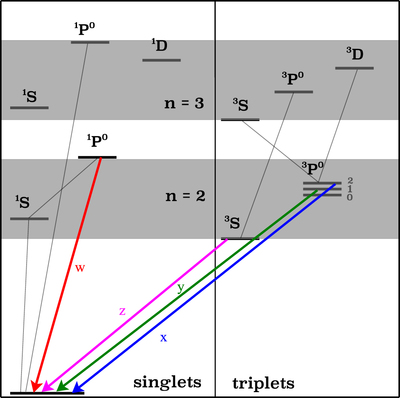
\includegraphics[clip=on,keepaspectratio,scale=3.5]{he_like_atom.jpg}
\end{center}
\end{figure}

\vspace{15 mm }
\LARGE
\emph{Cloudy \& Associates} \\
\Large
\href{http://www.nublado.org}{www.nublado.org} \\
\normalsize
\today
\end{center}
\end{titlepage}

%%%%%%%%%%%%%%%%%%%%%%%%%%%%%%%%%%%%%%%%%%%%%%%
% page with one figure and boilerplate text
\clearpage
{\small
\noindent
{\em Software:} Copyright \copyright\ 1978-2022 Gary J. Ferland and others. All rights reserved.

\vspace{1em}

\noindent
The software described in this documentation (\Cloudy) is subject
to a FreeBSD-style software license
contained in the file \cdFilename{license.txt} in the
root directory of the distributed files.
The list of co-authors is given in the file
\cdFilename{others.txt} in the same directory.
Use of this program is not restricted provided each use is
acknowledged upon publication.
The bibliographic reference to this version of \Cloudy\ is
``version xx.xx
of the code last described \citet{CloudyReview}.''
The version number, shown here as ``xx.xx'', should be
given.
This version number, along with a complete citation,
can be found by executing the code with the 
\cdCommand{print citation} command included in the input script.

\vspace{1em}

\noindent
\Cloudy\ is an evolving code.
You should confirm that you have the most recent
version of the code by checking the web site
\href{http://www.nublado.org}{www.nublado.org}.
The code has a
\href{https://cloudyastrophysics.groups.io}{discussion board} with emailing list.
This will have announcements of any updates to the code.\par

\vspace{1em}

\noindent
Portions of the documentation have been published, and are copyrighted by, the
American Astronomical Society, the Astronomical Society of the Pacific, and
the Royal Astronomical Society. The remainder of the documentation is subject
to the following FreeBSD format documentation license:

\vspace{1em}

\noindent
{\em Documentation:} Copyright \copyright\ 1978--2022 Gary J. Ferland and others. All rights reserved.

\vspace{1em}

\noindent
Redistribution and use of the documentation (all parts of \Hazy\ and the
Quick Start Guide) in source (\LaTeX) and `compiled' forms (PDF, PostScript,
HTML and so forth) with or without modification, are permitted provided that
the following conditions are met:

\begin{enumerate}
\item
Redistributions of source code (\LaTeX) must retain the above copyright notice,
this list of conditions and the following disclaimer as the first lines of
the file \cdFilename{license\_doc.txt} in the root directory unmodified.
\item
Redistributions in compiled form (converted to PDF, PostScript, XML, HTML and
other formats) must reproduce the above copyright notice, this list of
conditions and the following disclaimer in the documentation and/or other
materials provided with the distribution.
\end{enumerate}

\noindent
{\em This documentation is provided by the \Cloudy\ project ``as is'' and any express
or implied warranties, including, but not limited to, the implied warranties
of merchantability and fitness for a particular purpose are disclaimed. In no
event shall the  \Cloudy\  project be liable for any direct, indirect, incidental,
special, exemplary, or consequential damages (including, but not limited to,
procurement of substitute goods or services; loss of use, data, or profits; or
business interruption) however caused and on any theory of liability, whether
in contract, strict liability, or tort (including negligence or otherwise)
arising in any way out of the use of this documentation, even if advised of
the possibility of such damage.}\par
}

\vspace{5mm}
\noindent
{\small {\em Cover image:}
He-like atomic structure for the $n=2, 3$ configurations.
Figure 1 from \citet{Chakraborty2020b}.
}
\clearpage

%%%%%%%%%%%%%%%%%%%%%%%%%%%%%%%%%%%%%%%%%%%%%%%
% table of contents page - only include top two levels
\tableofcontents
\listoffigures
\listoftables

\clearpage
\mainmatter

% proofed 1 - read over latex file, remove dead xrefs,
% include figures, make xregs to figs and tables live
% NB the equations have not been checked
\chapter{THE MODEL ATOM FOR ISO-SEQUENCES}
% !TEX root = hazy3.tex

\section{Overview}

\Cloudy\ is designed to model environments that range from the low-density
limit to strict thermodynamic equilibrium.  Eventually all isoelectronic
series will be is treated as a multi-level atom plus continuum.   The
following chapters go over the H-like and He-like sequences.  This chapter
provides an overview.

Following sections are adapted from \citet{Ferland1988}, \citet{Ferland1989}, and \citet{FerlandPeterson1992}.

\section{Departure coefficients}

Departure coefficient is the ratio of the actual population of a state
to its population is thermodynamic equilibrium.  They are useful since they
allow direct comparison of a population to its asymptotic equilibrium limit.

The LTE relative population density for level $n$ is given by
\begin{equation}
\begin{array}{cl}
 {P_n}^*& = \frac{{n_n^*}}{{{n_e}{n_{ion}}}} =
\frac{{{g_n}}}{{{g_e}{g_{ion}}}}{\left(
{\frac{{m_n^*}}{{{m_e}\,{m_{ion}}}}\frac{{{h^2}}}{{2\pi \,kT}}}
\right)^{3/2}}\exp \left( { + {\chi _n}} \right) \\
&  \approx \frac{{{g_n}}}{{{g_e}{g_{ion}}}}{\left( {\frac{{{h^2}}}{{2\pi
\,{m_e}\,kT}}} \right)^{3/2}}\exp \left( { + {\chi _n}} \right) \\
&  = \frac{{{g_n}}}{{{g_e}{g_{ion}}}}4.1412957 \times {10^{ - 16}}{T^{ -
3/2}}\exp \left( { + {\chi _n}} \right) \\
 \end{array}
\mathrm{[cm^3]}
\end{equation}
where the electron statistical weight is $g_e = 2$, the ion statistical weights
are 1 and 2 for H-like and He-like species,
all nuclear statistical weights are ignored,
and $g_n = 2n^2$ is the statistical weight of hydrogenic level $n$.
$n_n*$ is the LTE population of level $n$~[$\pcc$ ],
and the other symbols have their usual meaning.
Here
\begin{equation}
{\chi _n} = \frac{{{I_n}}}{{kT}} = \frac{{15.7807 \times
{{10}^4}{Z^2}}}{{{n^2}T}}
\end{equation}
where $I_n$ is the ionization threshold for level $n$
and Z is the nuclear charge,
the exponent in equation 1 is positive,
and the last term holds for hydrogenic systems.
The dimensionless departure coefficients are related to the LTE
relative population density by
\begin{equation}
b_n = \frac{n_n}{P_n^* n_e n_{ion}}
\end{equation}
where $n_n$ is the actual population of the level.

\section{Pressure lowering of the ionization potential}

Not yet \dots.%[gjf1]

\section{Recombination rates and cooling}

This section is taken from \citet{Ferland1989}.

State-specific rates for radiative recombination and radiative
recombination cooling are needed for the temperature range
\TEMPLIMITLOW$ \le T \le $\TEMPLIMITHIGH.
The methods and assumptions used to derive these for hydrogenic ions
are described here.

\subsection{Formalism}

The Milne relation for the state-specific radiative recombination rate
coefficient (cm$^3$~s$^{-1}$) to a level $n$ can be expressed as
\citep{Brown1970}; \citealp{Gould1978}; \citealp{Mihalas1978});
\begin{equation}
\label{eqn:RecombinCoeffic}
\begin{array}{ccl}
 {\alpha _n}\left( T \right)& =& {\left( {\frac{{2\pi \,{m_e}k}}{{{h^2}}}}
\right)^{ - 3/2}}\frac{{8\pi }}{{{c^2}}}\frac{{{g_n}}}{{{g_e}{g_{ion}}}}{T^{
- 3/2}}\int_{h{\nu _o}}^\infty  {{\nu ^2}{\alpha _\nu }\left( n \right)}
\exp \left( { - h\left( {\nu  - {\nu _o}} \right)/kT} \right)\;d\nu  \\
&  =& 4.12373 \times {10^{11}}\frac{{{g_n}}}{{{g_e}{g_{ion}}}}{T^{ -
3/2}}\int_{h{\nu _o}}^\infty  {{\nu _{Ryd}}^2{\alpha _\nu }\left( n \right)}
\exp \left( { - h\left( {\nu  - {\nu _o}} \right)/kT} \right)\;d{\nu _{Ryd}}
\\
 \end{array}
\end{equation}
where the $g$'s are the statistical weights of the constituents,
$h\nu_{Ryd}$ is the photon energy in Rydbergs,
$h\nu_o \sim z^2/n^2$ is the ionization potential in Rydbergs,
$\alpha_\nu(n)$ is the photoionization cross section,
and the other symbols have their usual meanings.

In implementing this formalism the fact that, for hydrogen itself, the
energy scale is shifted by the ratio of the reduced mass of the nucleus
to an infinite mass was explicitly taken into account.  If the energy of
level $n$ of hydrogen is $n^{-2} R_{\mathrm{H}}$,
then the temperature corresponding to 1 Rydberg,
appearing in the exponential, is 157807~K,
not the commonly quoted 157890~K.
This does affect the results slightly since the energy scale
enters as an exponential in equation~\ref{eqn:RecombinCoeffic}.

Hydrogenic photoionization cross sections are required over a very wide
range of energy since recombination coefficients over a wide range of
temperature are needed.
Cross sections $\alpha_\nu(n)$ were calculated using a program
based on routines developed by \cite{Hummer1988},
\cite{Storey1991}, and Hummer (private communication).
The program generates the cross section values
at arbitrary photon energies for all hydrogenic ($n$,l) states, as well as
for the total $n$, employing analytic expressions and some very accurate
expansions and numerical procedures.  The calculations were carried out
at a number of different mesh sizes to check for convergence.  The results
are typically accurate to better than 0.1 percent.

The recombination cooling rate coefficient (erg cm$^3$~s$^{-3}$)
is given by
\begin{equation}
kT\beta \left( {t,n} \right) = {\left( {\frac{{2\pi {m_e}k}}{{{h^2}}}}
\right)^{ - 3/2}}\frac{{8\pi }}{{{c^2}}}\frac{{{g_n}}}{{{g_e}{g_{ion}}}}{T^{
- 3/2}}\int_{h{\nu _o}}^\infty  {{\nu ^2}\;{\alpha _\nu }\left( n
\right)\;h\left( {\nu  - {\nu _o}} \right)\;\exp \left( { - h\left( {\nu
- {\nu _o}} \right)/kT} \right)\;d\nu }
\end{equation}

\subsection{Results}

%   Table 1
\begin{table}
\label{tab:RecombinCoeffic}
\caption{State Specific and Case B Recombination Coefficients}
\begin{tabular}{llllllll}
\hline
log(T$_e$)& 1&  2&  3&  4&  5&  6&  Case B\\
\hline
0.5& 9.258-12&
5.087-12& 3.512-12& 2.684-12& 2.172-12& 1.825-12& 5.758-11\\
1.0&
5.206-12& 2.860-12& 1.974-12& 1.508-12& 1.220-12& 1.025-12& 2.909-11\\
1.5&  2.927-12& 1.608-12& 1.109-12& 8.465-13& 6.842-13& 5.737-13&
1.440-11\\
2.0& 1.646-12& 9.028-13& 6.216-13& 4.732-13& 3.811-13&
3.183-13& 6.971-12\\
2.5& 9.246-13& 5.055-13& 3.460-13& 2.613-13&
2.084-13& 1.720-13& 3.282-12\\
3.0& 5.184-13& 2.805-13& 1.888-13&
1.395-13& 1.085-13& 8.717-14& 1.489-12\\
3.5& 2.890-13& 1.517-13&
9.779-14& 6.884-14& 5.099-14& 3.912-14& 6.430-13\\
4.0& 1.582-13&
7.699-14& 4.555-14& 2.965-14& 2.053-14& 1.487-14& 2.588-13\\
4.5&
8.255-14& 3.461-14& 1.812-14& 1.076-14& 6.953-15& 4.775-15& 9.456-14\\
5.0& 3.882-14& 1.316-14& 6.059-15& 3.314-15& 2.022-15& 1.331-15&
3.069-14\\
5.5& 1.545-14& 4.196-15& 1.736-15& 8.918-16& 5.219-16&
3.335-16& 8.793-15\\
6.0& 5.058-15& 1.146-15& 4.392-16& 2.160-16&
1.229-16& 7.694-17& 2.245-15\\
6.5& 1.383-15& 2.760-16& 1.005-16&
4.807-17& 2.685-17& 1.660-17& 5.190-16\\
7.0& 3.276-16& 6.031-17&
2.129-17& 1.000-17& 5.523-18& 3.385-18& 1.107-16\\
7.5& 7.006-17&
1.227-17& 4.251-18& 1.976-18& 1.083-18& 6.606-19& 2.221-17\\
8.0&
1.398-17& 2.377-18& 8.139-19& 3.759-19& 2.052-19& 1.248-19& 4.267-18\\
8.5&  2.665-18& 4.455-19& 1.515-19& 6.970-20& 3.796-20& 2.303-20&
7.960-19\\
9.0& 4.940-19& 8.175-20& 2.769-20& 1.271-20& 6.913-21&
4.190-21& 1.457-19\\
9.5& 9.001-20& 1.481-20& 5.005-21& 2.294-21&
1.247-21& 7.552-22& 2.636-20\\
10.0& 1.623-20& 2.662-21& 8.985-22&
4.116-22& 2.235-22& 1.354-22& 4.737-21\\
\hline
\end{tabular}
\end{table}

\begin{table}
\label{tab:RecombinCoolingCoeffic}
\caption{State Specific and Case B Recombination Cooling Coefficients}
\begin{tabular}{llllllll}
\hline
log(T$_e$)& 1&  2&  3&  4&  5&  6&  case B\\
\hline
0.5& 4.025-27&
2.211-27& 1.527-27& 1.167-27& 9.441-28& 7.929-28& 2.295-26\\
1.0&
7.158-27& 3.932-27& 2.713-27& 2.072-27& 1.676-27& 1.406-27& 3.595-26\\
1.5&      1.273-26& 6.985-27& 4.815-27& 3.671-27& 2.962-27& 2.479-27&
5.514-26\\
2.0&      2.262-26& 1.239-26& 8.507-27& 6.451-27& 5.171-27&
4.293-27& 8.236-26\\
2.5 &     4.015-26& 2.184-26& 1.483-26& 1.107-26&
8.708-27& 7.074-27& 1.187-25\\
3.0&      7.099-26& 3.785-26& 2.488-26&
1.784-26& 1.341-26& 1.039-26& 1.629-25\\
3.5&      1.241-25& 6.245-26&
3.796-26& 2.505-26& 1.740-26& 1.255-26& 2.082-25\\
4.0&      2.094-25&
9.195-26& 4.856-26& 2.845-26& 1.795-26& 1.198-26& 2.395-25\\
4.5&
3.234-25& 1.112-25& 4.923-26& 2.557-26& 1.483-26& 9.305-27& 2.376-25\\
5.0&      4.173-25& 1.056-25& 3.990-26& 1.891-26& 1.034-26& 6.240-27&
1.981-25\\
5.5&      4.149-25& 7.981-26& 2.698-26& 1.208-26& 6.389-27&
3.771-27& 1.390-25\\
6.0&      3.121-25& 4.961-26& 1.572-26& 6.827-27&
3.549-27& 2.073-27& 8.316-26\\
6.5&      1.843-25& 2.616-26& 8.015-27&
3.429-27& 1.768-27& 1.028-27& 4.307-26\\
7.0&      9.016-26& 1.204-26&
3.628-27& 1.541-27& 7.917-28& 4.591-28& 1.967-26\\
7.5&      3.847-26&
4.978-27& 1.487-27& 6.296-28& 3.229-28& 1.870-28& 8.109-27\\
8.0&
1.490-26& 1.897-27& 5.644-28& 2.385-28& 1.222-28& 7.077-29& 3.092-27\\
8.5&      5.397-27& 6.811-28& 2.023-28& 8.541-29& 4.375-29& 2.533-29&
1.115-27\\
9.0&      1.867-27& 2.346-28& 6.959-29& 2.937-29& 1.504-29&
8.706-30& 3.872-28\\
9.5&      6.261-28& 7.849-29& 2.327-29& 9.820-30&
5.028-30& 2.910-30& 1.316-28\\
10.0&      2.057-28& 2.575-29& 7.633-30&
3.220-30& 1.649-30& 9.543-31& 4.436-29\\
\hline
\end{tabular}
\end{table}

The numerical results are presented in Tables \ref{tab:RecombinCoeffic}
and \ref{tab:RecombinCoolingCoeffic}.
The first column
of the table gives the log of the temperature.  Columns 2 through 7 give
the total recombination coefficient for $1 \le n \le 6$ summed over $l$ states. The
last column gives the case B sum, $2\le  n\le  1000$.  A very large temperature
range is considered for completeness; actually, at very low temperatures
three-body recombination predominates for most densities
\citep{Bates1962},
while at very high temperatures other processes (i.e., Compton scattering,
collisions) dominate the balance and the neutral fraction is vanishingly
small.

As tests, these predictions of the recombination rate coefficients are
compared with those of \citep{Seaton1959a},
\citep{Ferland1980c}, \citep{Hummer1987}, and \citet{Martin1988}.
Note that the total recombination rate given
by Hummer and Storey is the sum of radiative and net three-body
recombination.  For this comparison their results for a density of
$10^2 \pcc$
were used to minimize the contribution of the second process.  The agreement
with all of these results is good, usually much better than 1 percent.
\citep{Seaton1959a} calculates the recombination cooling coefficients.
The present
results agree with his to better than 5 percent.
Figure \ref{fig:HRecomCooling} shows the recombination-cooling coefficient for several states.

\begin{figure}
\label{fig:HRecomCooling}
\centering
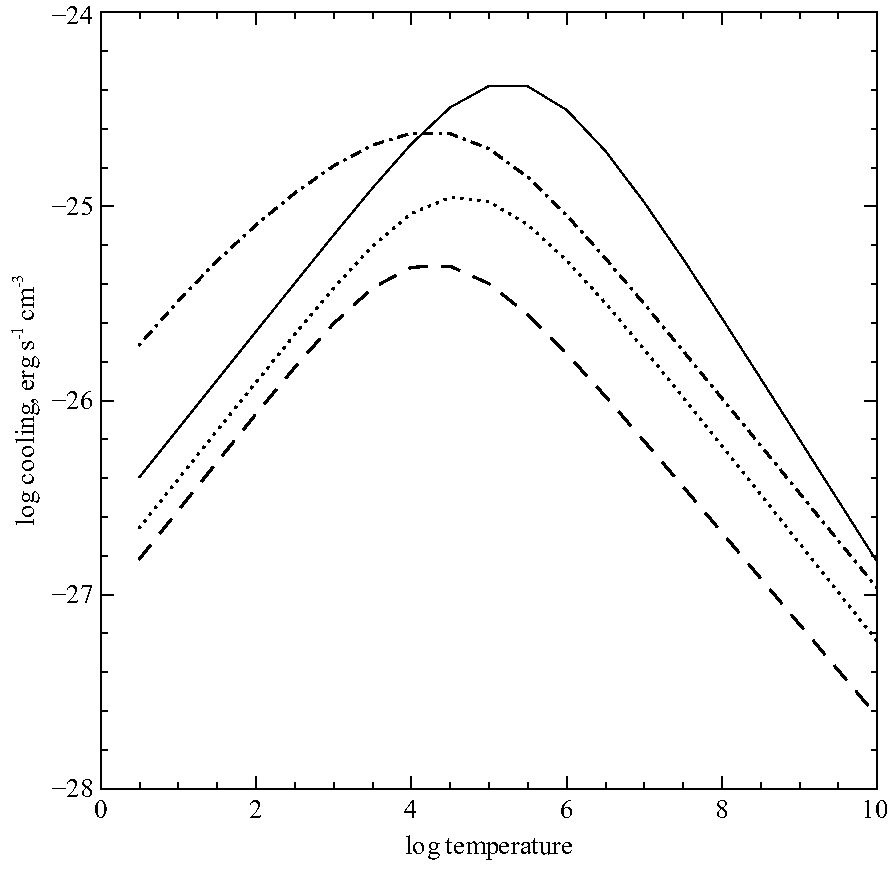
\includegraphics[scale=0.8]{HRecomCooling}
\caption[H recombination cooling]{The recombination cooling for several states is shown as a function
of temperature.}
\end{figure}

\section{The collisional rate equations}

The collision rates between two terms in strict
thermodynamic equilibrium (STE) are related by detailed
balance.  Then
\begin{equation}
n_l^*{C_{l,u}} = n_u^*{C_{u,l}}
\end{equation}
and we get the usual relation between collisional excitation and
de-excitation rates,
\begin{equation}
{C_{l,u}} = \left( {n_u^*/n_l^*} \right){C_{u,l}} = \left( {{g_u}/{g_l}}
\right)\exp \left( { - \chi /kT} \right){C_{u,l}}.
\end{equation}

Considering only collisional terms, the departure coefficient for level
$n$ is given by
\begin{equation}
\frac{{d{b_n}}}{{dt}} = \sum\limits_l {{b_l}{C_{n,l}} + \sum\limits_u
{\frac{{P_u^*}}{{P_n^*}}{b_u}{C_{u,n}} - {b_n}\left\{ {\sum\limits_l
{{C_{n,l}}}  + \sum\limits_u {\frac{{P_u^*}}{{P_n^*}}{C_{u,n}} +
{C_{n,k}}\left( {1 - b_n^{ - 1}} \right)} } \right\}} }
\end{equation}
where the sums are over upper and lower levels.
The collision rates
($\ps$)
from level $i$ to level $j$ are denoted by $C_{ij}$.
The first term on the RHS
represents collisional excitation to $n$ from lower levels, the second is
collisional deexcitation to $n$ from higher levels,
and the last term accounts
for destruction processes.
These include collisions to lower levels, upper
levels, and the continuum.
The factor multiplying the collisional ionization
rate $C_{n\kappa}$ accounts for collisional ionization less three-body recombination.
Note that this is often a net recombination process for the atom since,
under many circumstances, $b_n < 1$.

Figure \ref{fig:HDepartCoefVsDensity} shows a test case where collisional processes are dominant.
All of the radiative processes discussed below are actually included, but
the intensity of the external continuum is set to a very low (and hence
negligible) value.  As a result collisional and spontaneous radiative
processes are dominant.  The electrons are given a temperature of 50000
K, and the level populations and ionization of the gas are determined by
solving the full set of equations of statistical equilibrium.  The model
is of a very thin cell of gas that is optically thin in the lines and
continuum.  Departure coefficients for the ground state, 2s, 2p, and 4 are
shown.

\begin{figure}
\label{fig:HDepartCoefVsDensity}
\centering
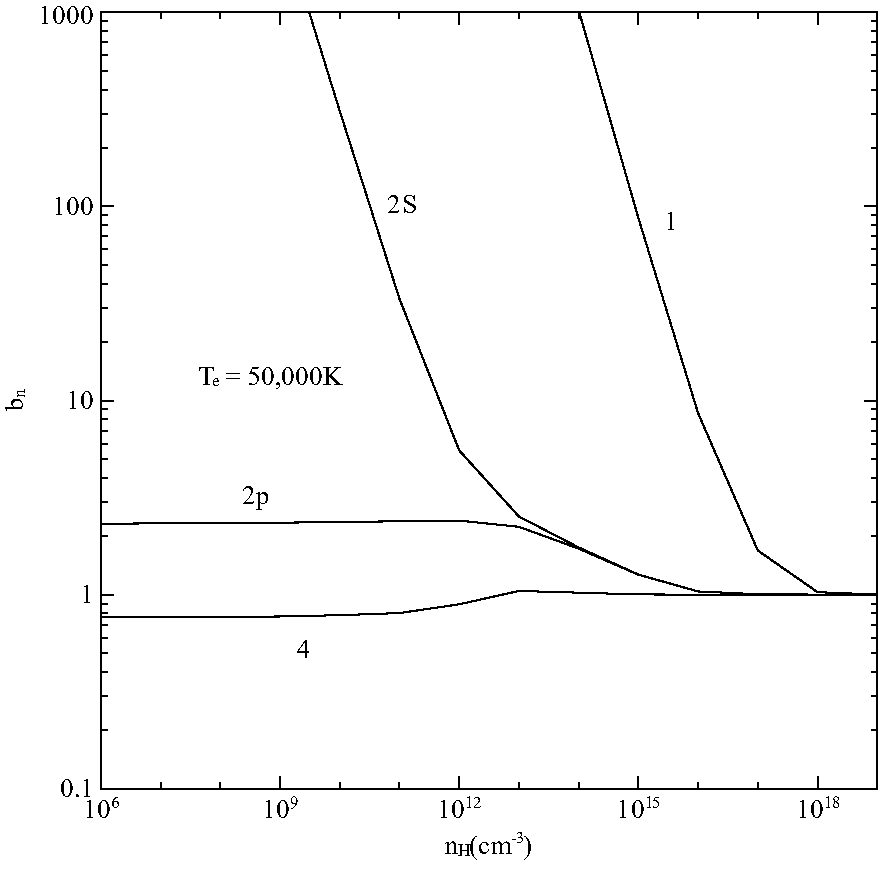
\includegraphics[scale=0.8]{HDepartCoefVsDensity}
\caption[H populations vs density]{The equilibrium populations of the ground state and levels  $2s$,
$2p$, and 4 of the model hydrogen atom
are shown as a function of the total
hydrogen density n$_{\mathrm{H}}$.}%
\end{figure}

The radiation field is set to a very low intensity, and the column density
is kept small enough for optical depth effects to be negligible.  A constant
electron temperature of $5\times  10^4 \K$ is assumed, so the gas is primarily
collisionally ionized and excited.
Levels $2s$ and $2p$ do not mix until a
density of nearly $10^{14} \pcc$ is reached,
and do not come into LTE until the
density is nearly 100 times higher.
The entire atom is nearly in LTE at
densities greater than $10^{18} \pcc$

The ground state is overpopulated relative to its LTE value when upward
collisional processes are much slower than downward radiative processes.
It is only when the collisional rates approach the radiative rates that
$b_1$ approaches unity.
The $2s$ level also has a large overpopulation for much
the same reason.  It is highly metastable and accumulates a large
overpopulation until $2s -- 2p$ collisions become fast enough
to mix the two $l$ levels.
The more highly excited levels ($n\ge  3$) have a behavior very similar
to that of $n=4$, which is shown in the figure.  They are under populated
relative to their LTE value when radiative decays to lower levels are
competitive with collisional processes.
It is only at a density of $n_H > 10^{18} \pcc$ that collisional processes completely dominate the rate equations
and the atom reaches LTE.
The mean departure coefficient at a density of
$10^{19} \pcc$ is ${\bar b_i} = 1.0007 \pm 0.0022$
for the entire atom, and the largest single deviation from unity is
0.7\% (for the ground level).

\section{The radiative rate equations}

\subsection{Photoionization---recombination}

The photoionization rate ($\ps$) is given by
\begin{equation}
{\Gamma _n} = 4\pi \,\int_{{\nu _o}}^\infty  {\frac{{{J_\nu }}}{{h\nu
}}\;{\alpha _\nu }\;d\nu }\quad [\mathrm{s}^{-1}]
\end{equation}
and the induced recombination rate coefficient by
\begin{equation}
\label{eqn:InducedRecombinationRateCoefficient}
\alpha \left( {ind} \right) = P_n^*4\pi \int_{{\nu _o}}^\infty
{\frac{{{J_\nu }}}{{h\nu }}\;{\alpha _\nu }\exp \left( { - h\nu /kT}
\right)\;d\nu }\quad  [\mathrm{cm}^3 \mathrm{s}^{-1}].
\end{equation}
This is evaluated at each zone by direct integration.

The ground level also includes destruction due to bound Compton scattering.

\subsection{Derivation of radiative balance equations}

Consider the balance for a level $n$ of a three level system, with upper
and lower levels $u$ and~$l$.
\begin{equation}
{n_n}\left( {{B_{n,u}}\bar J + {B_{n,l}}\bar J + {A_{n,l}}} \right) =
{n_u}\left( {{B_{u,n}}\bar J + {A_{u,n}}} \right) + {n_l}{B_{l,n}}\bar J.
\end{equation}
Converting densities ni into departure coefficients, ${n_i} = {b_i}P_i^*$, we obtain
\begin{equation}
P_n^*{b_n}\left( {{B_{n,u}}\bar J + {B_{n,l}}\bar J + {A_{n,l}}} \right)
= P_u^*{b_u}\left( {{B_{u,n}}\bar J + {A_{u,n}}} \right) +
P_l^*{b_l}{B_{l,n}}\bar J.
\end{equation}
Gathering LTE densities we find
\begin{equation}
{b_n}\left( {{B_{n,u}}\bar J + {B_{n,l}}\bar J + {A_{n,l}}} \right) =
\frac{{P_u^*}}{{P_n^*}}{b_u}\left( {{B_{u,n}}\bar J + {A_{u,n}}} \right)
+ \frac{{P_l^*}}{{P_n^*}}{b_l}{B_{l,n}}\bar J.
\end{equation}
Writing $B_{ln} = B_{nl} g_n/g_l$, we obtain the final form
\begin{equation}
{b_n}\left( {\frac{{{g_u}}}{{{g_n}}}{B_{u,n}}\bar J + {B_{n,l}}\bar J
+ {A_{n,l}}} \right) = \frac{{P_u^*}}{{P_n^*}}{b_u}\left( {{B_{u,n}}\bar
J + {A_{u,n}}} \right) +
\frac{{P_l^*}}{{P_n^*}}{b_l}\frac{{{g_n}}}{{{g_l}}}{B_{n,l}}\bar J.
\end{equation}

\subsection{Final radiative equations}

The full set of radiative balance equations can be written as
\begin{equation}
\begin{array}{ccc}
 \frac{{d{b_n}}}{{dt}}& = & \sum\limits_l
{\frac{{P_l^*}}{{P_n^*}}{b_l}{A_{n,l}}\frac{{{g_n}}}{{{g_l}}}\,{\eta
_{n,l}}{\gamma _{n,l}} + \sum\limits_u {\frac{{P_u^*}}{{P_n^*}}{b_u}\left(
{{A_{u,n}}{P_{u,n}} + {A_{u,n}}{\eta _{u,n}}{\gamma _{u,n}}} \right)} }
+  \\
&&
 \left[ {\alpha \left( {rad} \right) + \alpha \left( {ind} \right)}
\right]/P_n^* -  \\
&&
 {b_n}\left( {\sum\limits_l {\left( {{A_{n,l}}{P_{n,l}} + {A_{n,l}}{\eta
_{n,l}}{\gamma _{n,l}}} \right) + \sum\limits_u
{{A_{u,n}}\frac{{{g_u}}}{{{g_n}}}{\eta _{u,n}}{\gamma _{u,n}} + {\Gamma
_n}} } } \right) \\
 \end{array}
\end{equation}
where the $\eta$ is the continuum occupation number in the transition $ij$.

Figure \ref{fig:HDepartCoefVsRadiationField} shows a test case that,
in contrast to that shown in Figure
\ref{fig:HDepartCoefVsDensity},
is dominated by radiative transitions.

\begin{figure}
\label{fig:HDepartCoefVsRadiationField}
\centering
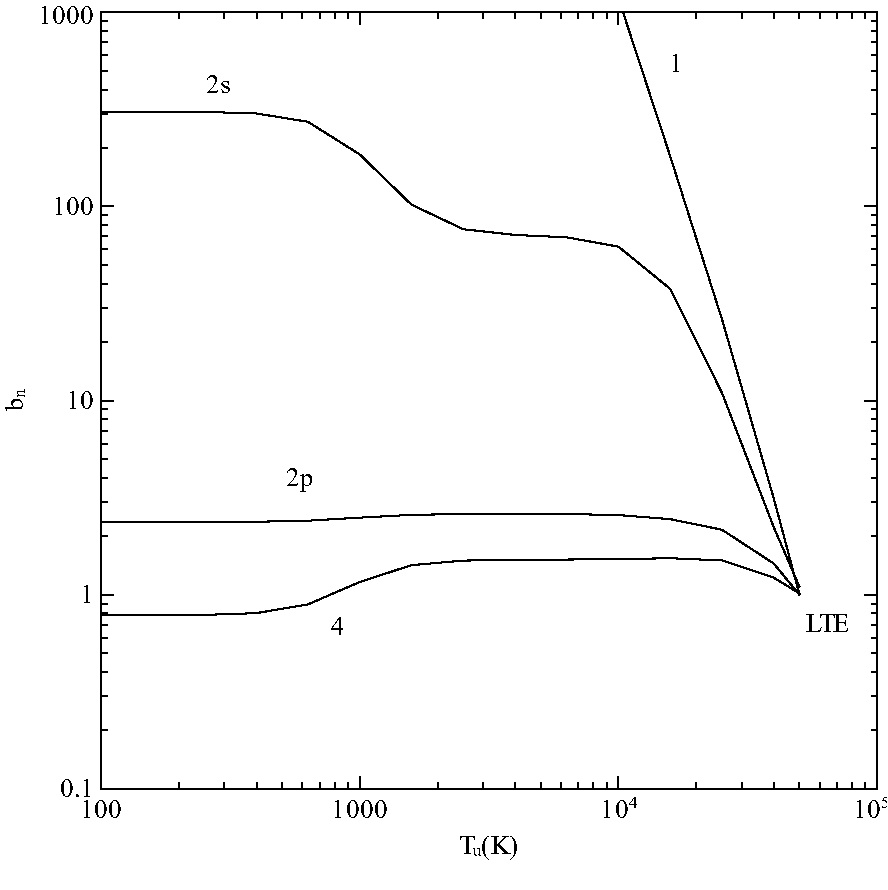
\includegraphics[scale=0.8]{HDepartCoefVsRadiationField}
\caption[H populations vs radiation field]{The calculations are for a constant temperature $(T = 5 \times
10^4 K)$
optically thin gas exposed to black body radiation with a color temperature
of $T_{color} = 5 \times 10^4 K$, but with various values of the energy density,
parameterized as $T_u = (u/a)^{1/4}$, where u is the actual radiation
density.}
\end{figure}

Again, the full set of equations coupling the levels are solved, but
spontaneous and induced processes are more important than collisions for
many values of the radiation density.  The model is of a very thin cell
of gas, so that all lines and continua are optically thin, has a density
of $n(H) = 10^{10}$~cm$^{-3}$, and an electron temperature of $5 \times
10^4$~K.
The gas is
exposed to a black body continuum with a color temperature of
$T_{color} = 5
\times 10^4$~K, but the intensity of this continuum is varied.  This intensity is
parameterized by an energy density temperature defined by $T_u \equiv
(u/a)^{1/4}$ where
$u$ and $a$ are, respectively, the actual radiation energy density and Stefan's
radiation density constant.

A radiation field given by Planck's law (i.e., $T_u\equiv  T_{color}$) forces the
ionization and level population of an atom or ion to LTE in much the same
way that high electron densities do.
As Figure \ref{fig:HDepartCoefVsRadiationField} shows, at very low values
of $T_u$ (low photon densities) the ground and $n = 2$ states are overpopulated
for much the same reason that this occurs at low electron densities; the
downward spontaneous radiative rates are fast relative to the induced (upward
and downward) rates.  At very low $T_u (< 500 \K), n \ge 3$ levels are under
populated since they decay at a rate much faster than the induced rates
(for $T = 5 \times 10^4$~K these levels have $h\nu? kT$, so induced processes will be
fast relative to spontaneous rates when $T_u = T_{color}$ and the atom is in LTE).
As $T_u$ increases, fluorescence from the ground state over-populates excited
states (because the ground state is itself overpopulated) and $b_4$ exceeds
unity.  Finally, in the limit where $T_u = T_{color}$, the departure coefficients
reach unity and the atom goes to LTE.  (The actual mean departure coefficient
for the entire atom is ${\bar b_i} = 1.013 \pm 0.029$).  Note that the vast majority of the neutral hydrogen population is
in excited states when the atom approaches LTE at these temperatures.

The hydrogen density $(n(H) = 10^{10}$~cm$^{-3}$) is low enough for radiation to
be the main agent affecting level populations for most values of $T_u$.
Fluorescence from the ground state drives the population of $n=4$ above its
LTE value for many radiation densities.  Induced processes, mainly
transitions between adjacent levels, drive the atom to LTE when $T_u$ reaches
$5 \times 10^4$~K.


   %proof 1
\chapter{THE HYDROGENIC ISO-SEQUENCE}
% !TEX root = hazy3.tex

Tests in the low-density, or nebular, limit show that the model atom predicts
level populations and emissivities that are in much better than 1\% agreement
with Seaton (1959), and with the Storey and Hummer (1995) results.  The
atom goes to LTE in the high radiation or matter density limits.

\section{Recombination rates and cooling}

\subsection{Rational approximations}%[gjf1]

It is not numerically expedient to compute these rate coefficients on-the-fly
in large scale ionization/thermal structure calculations.  The rate
coefficients were fitted with a high-order rational approximation.  The
recombination rate coefficient is expressed~as
\begin{equation}
\alpha \left( {n,T} \right) = {10^{F(n,T)}}\;{T^{ - 1}}
\end{equation}
with
\begin{equation}
F(n,T) = \frac{{{a_n} + {c_n}x + {e_n}{x^2} + {g_n}{x^3} + {i_n}{x^4}}}{{1
+ {b_n}x + {d_n}{x^2} + {f_n}{x^3} + {h_n}{x^4}}}
\end{equation}
and $x \equiv \log$(T).  These approximations reproduce the numerical results with
a mean error well below 0.1 percent.  For levels below $n=20$ the largest
error is also under 0.1 percent, although errors as large as 1.4 percent
occur for the highest sum at temperatures below 100~K.

Recombination cooling coefficients were fitted to equations of the form
\begin{equation}
kT\beta \left( {n,T} \right) = {10^{F(n,T)}}
\end{equation}
where $F(T,n)$ is given above, and the fitting coefficients are given in the
code.  The errors in fitting these coefficients are larger, typically 0.5
percent, but sometimes as large as several percent.

\section{Effective transition probabilities}

\subsection{Einstein As}

Two routines are used to compute hydrogenic transition probabilities, in
the limit of a completely $l$-mixed atom.  There routines were coded by Jason
Ferguson, using algorithms given by \citet{Johnson1972}.

Note that the code considers the $2s$ and $2p$ as two separate levels.  These
routines return transition probabilities for a well $l$-mixed atom, and cannot
be applied directly to the separate $2s$ and $2p$ levels.

\section{Collisional contributions to hydrogen lines}

Figure \ref{fig:HLinesFerlandOsterbrock},
taken from Ferland \& Osterbrock (1985), shows the effects of
collisional excitation on hydrogen lines.  This process can be significant
relative to recombination when the gas temperature is high (perhaps due
to low metallicity) or in partially neutral gas that is exposed to x-rays.
The lines marked ``external'' are reddening curves due to external dust,
and ``internal'' tracks the effects of internal dust.  The band of solutions
that go across the top of the figure shows the expected hydrogen line
spectrum, as set by the collision strengths of the Lyman lines.

\begin{figure}
\centering
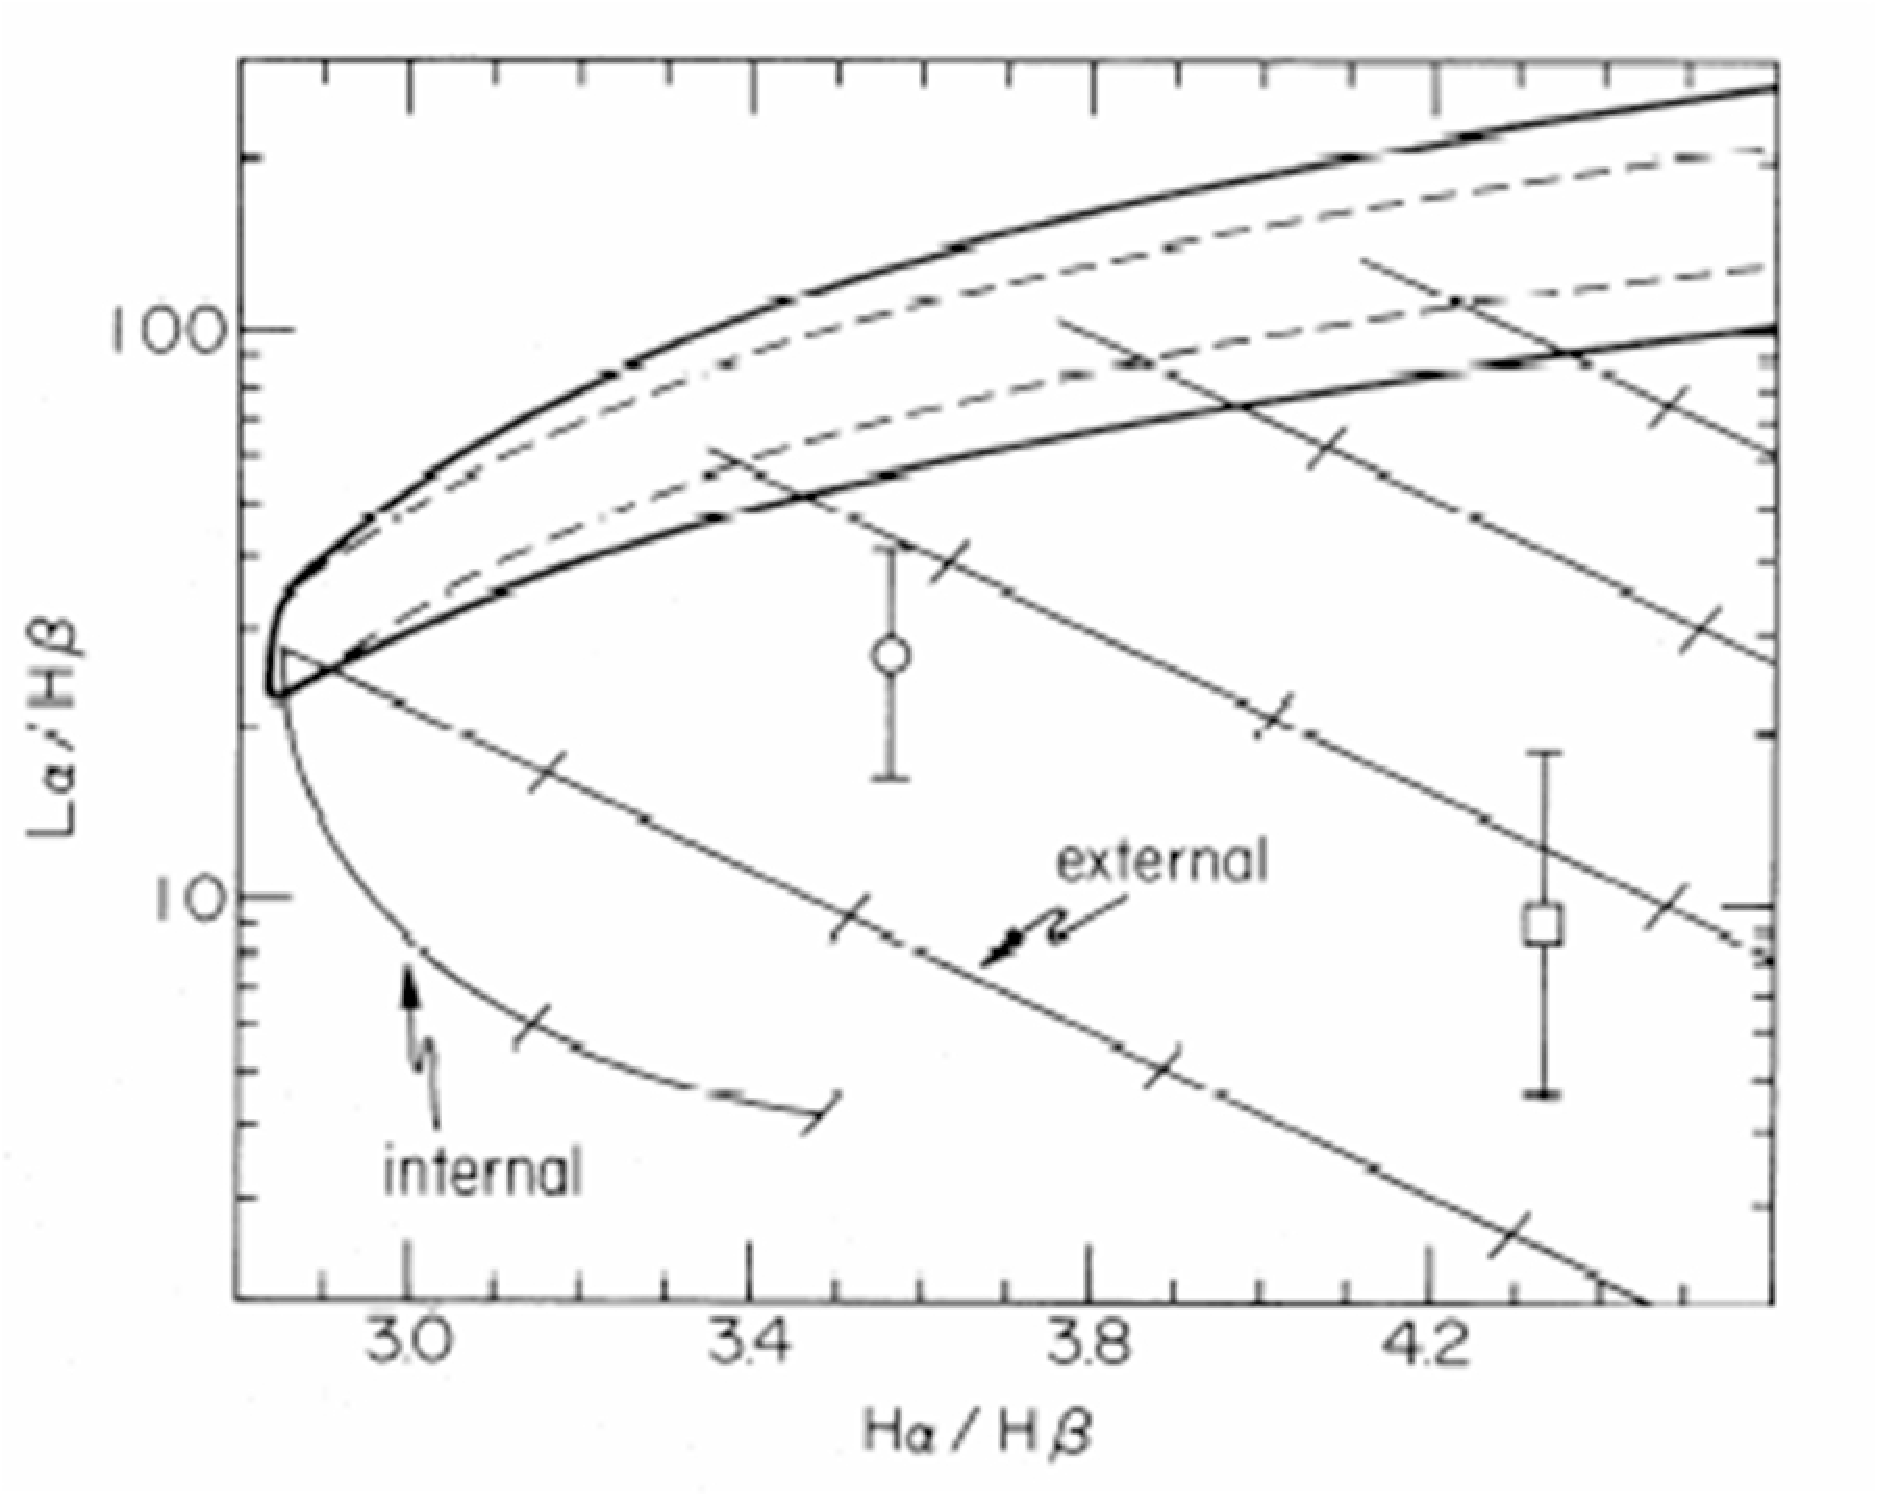
\includegraphics[scale=0.4]{HLinesFerlandOsterbrock}
\label{fig:HLinesFerlandOsterbrock}
\caption[Hydrogen line ratios]
{This figure, taken from Ferland \& Osterbrock 1985, shows the
effects of collisional excitation upon two ratios of hydrogen lines.  The
largest effects are to enhance \la\ and \ha\ by large amounts. }
\end{figure}

\section{Continuous thermal emission}

Diffuse emission (free-free and free-bound) by all atoms is computed using
the stored photoabsorption cross sections and detailed balance (i.e., the
Milne relation; see \citealp{Mihalas1978}).

Free-bound continua of all levels of hydrogen and helium are treated as
follows.  The Milne relation for the emissivity $4\pi j$ (erg~cm$^3$
Hz$^{-1}$~s$^{-1}$) can
be expressed as \citep{Brown1970}
\begin{equation}
r\pi j_\nu = h\nu \left(\frac{2\pi m_ck}{h^2}\right)^{3/2} \frac{8\pi}{c^2}
\frac{g_n}{g_eg_{ion}} T^{-3/2}\nu^2 \alpha_\nu (n) \exp
\left(-h(\nu-\nu_o)/kT\right)
\end{equation}
where the statistical weight of level $n$ is $g_n = 2n^2$ for $H^0$ and
He$^+$, and
$g_n = n^2$ for helium singlets.

The code actually works with units similar to photons
Ryd$^{-1}$~s$^{-1}$~cm$^{-2}$.  The
photon emissivity (photons cm$^3$ s$^{-1}$ Ryd$^{-1}$) is then
\begin{equation}
\label{eqn:HPhotonEmissivity}
\begin{array}{ccc}
 {\varphi _\nu }\left( {T,n} \right)&  =& {\left( {\frac{{2\pi
\,{m_e}k}}{{{h^2}}}} \right)^{ - 3/2}}\;\frac{{8\pi
}}{{{c^2}}}\;\frac{{{g_n}}}{{{g_e}{g_{ion}}}}\;{T^{ - 3/2}}\;{\nu ^2}{\alpha
_\nu }\left( n \right)\exp \left( { - h\left( {\nu  - {\nu _o}} \right)/kT}
\right) \\
&=& 4.12373 \times {10^{11}}\frac{{{g_n}}}{{{g_e}{g_{ion}}}}\;{T^{ -
3/2}}\;{\nu _{Ryd}}^2{\alpha _\nu }\left( n \right)\,\exp \left( { - h\left(
{\nu  - {\nu _o}} \right)/kT} \right) \\
 \end{array}
\end{equation}
where the $g$'s are the statistical weights of the constituents, $\nu_{Ryd}$ is the
photon energy in Rydbergs, $h\nu_o\sim z^2/n^2$ is the ionization potential in Rydbergs,
$\alpha_\nu(n)$ is the photoionization cross section, and the other symbols have their
usual meanings.
Equation \ref{eqn:HPhotonEmissivity} is evaluated directly using the stored
photoionization cross sections.  A similar approach is used for all
absorption opacities.  Detailed balancing between absorption and emission
mechanisms is necessary if LTE is to be achieved.

A test case with an ionized hydrogen plasma at a temperature
of $10^4 \K$ and
a density of $10^7~\pcc$
(to suppress two photon emission) was computed, and
is shown in Figure~\ref{fig:HemisCompareFerland80}.

\begin{figure}
\centering
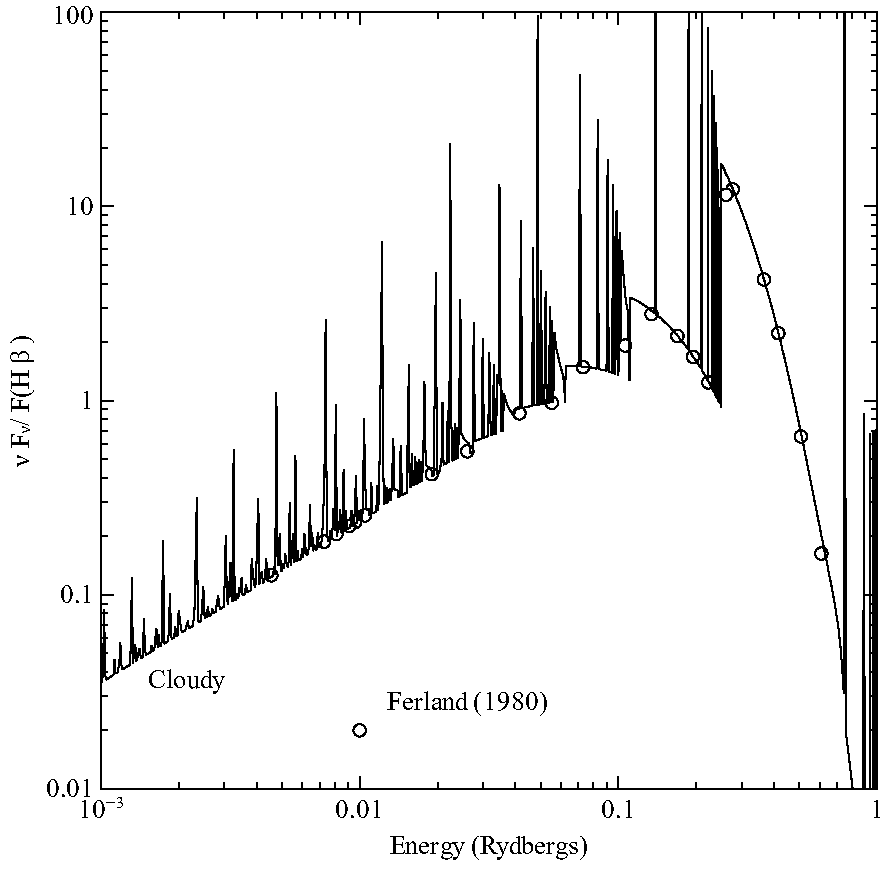
\includegraphics[scale=0.8]{HemisCompareFerland80}
\caption[H emission comparision]{\label{fig:HemisCompareFerland80}
The emission from a slab of gas is compared with the
predictions of \citet{Ferland1980c}.}%  hemis computed Page: 212
\end{figure}
%97 jan 3, using 90.02l

The input stream used to derive the figure is included in the test suite.
As can be seen from this figure, the predicted diffuse continuum is generally
within a percent of the exact value (given in \citealt{Ferland1980c}).

Figure \ref{fig:HConEmissBBLimit} shows another series of test cases in which a very high density
gas with cosmic abundances is irradiated with a 5\e{4} K blackbody radiation
field in strict thermodynamic equilibrium.  As can be seen from the figure,
the predicted continuum goes to the blackbody limit.

%Figure 4
\begin{figure}
\centering
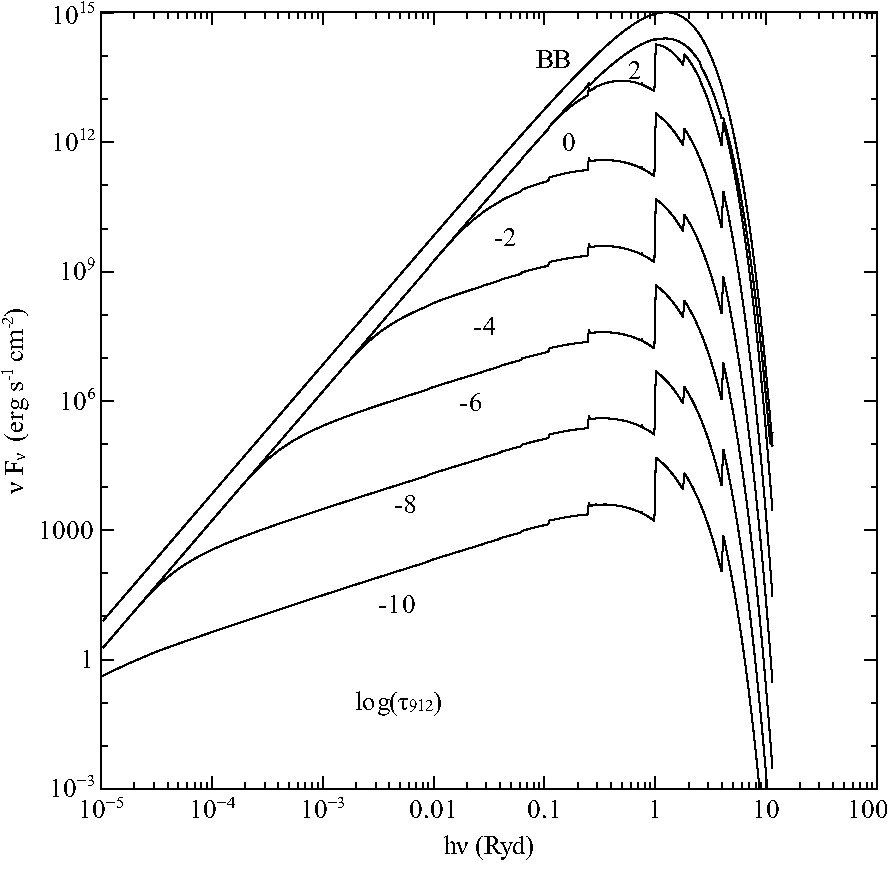
\includegraphics{HConEmissBBLimit}
\caption[H emission in black body limit]
{\label{fig:HConEmissBBLimit}The emission from a dense slab of gas with cosmic abundances is
shown as a function of the optical depth at the Lyman limit.  The log of
this optical depth is indicated on the figure.  The top curve is for emission
given by Planck's law.  The continuous emission goes to the blackbody limit
in the case of large continuum optical depths.}
\end{figure}

 %proof 1
\chapter{HELIUM ISO-SEQUENCE}
% !TEX root = hazy3.tex

\section{Overview}

The helium-like isoelectronic sequence is treated with a single unified
approach that was developed by Ryan Porter as his PhD thesis.  These are
published in \citet{Bauman2005}, \citet{Porter2005}, Porter et al.
(2007), and \citet{PorterFerland2007}

\section{Energy levels}

Figure \ref{fig:helium_energy_levels} shows a partial
Grotrian diagram for He-like ions.
The order of the $J$ levels within $2p\;{P^o}$
is reversed for the atom; the energy levels shown in
Figure \ref{fig:helium_energy_levels} are for
astrophysically abundant ions.  In the code the energies associated with
a particular $J$ level are always correct, but for He I these occur out of
order in the vector of energy levels.  This is ok since the levels are so
close to having the same energy.

\begin{figure}
\centering
\label{fig:helium_energy_levels}
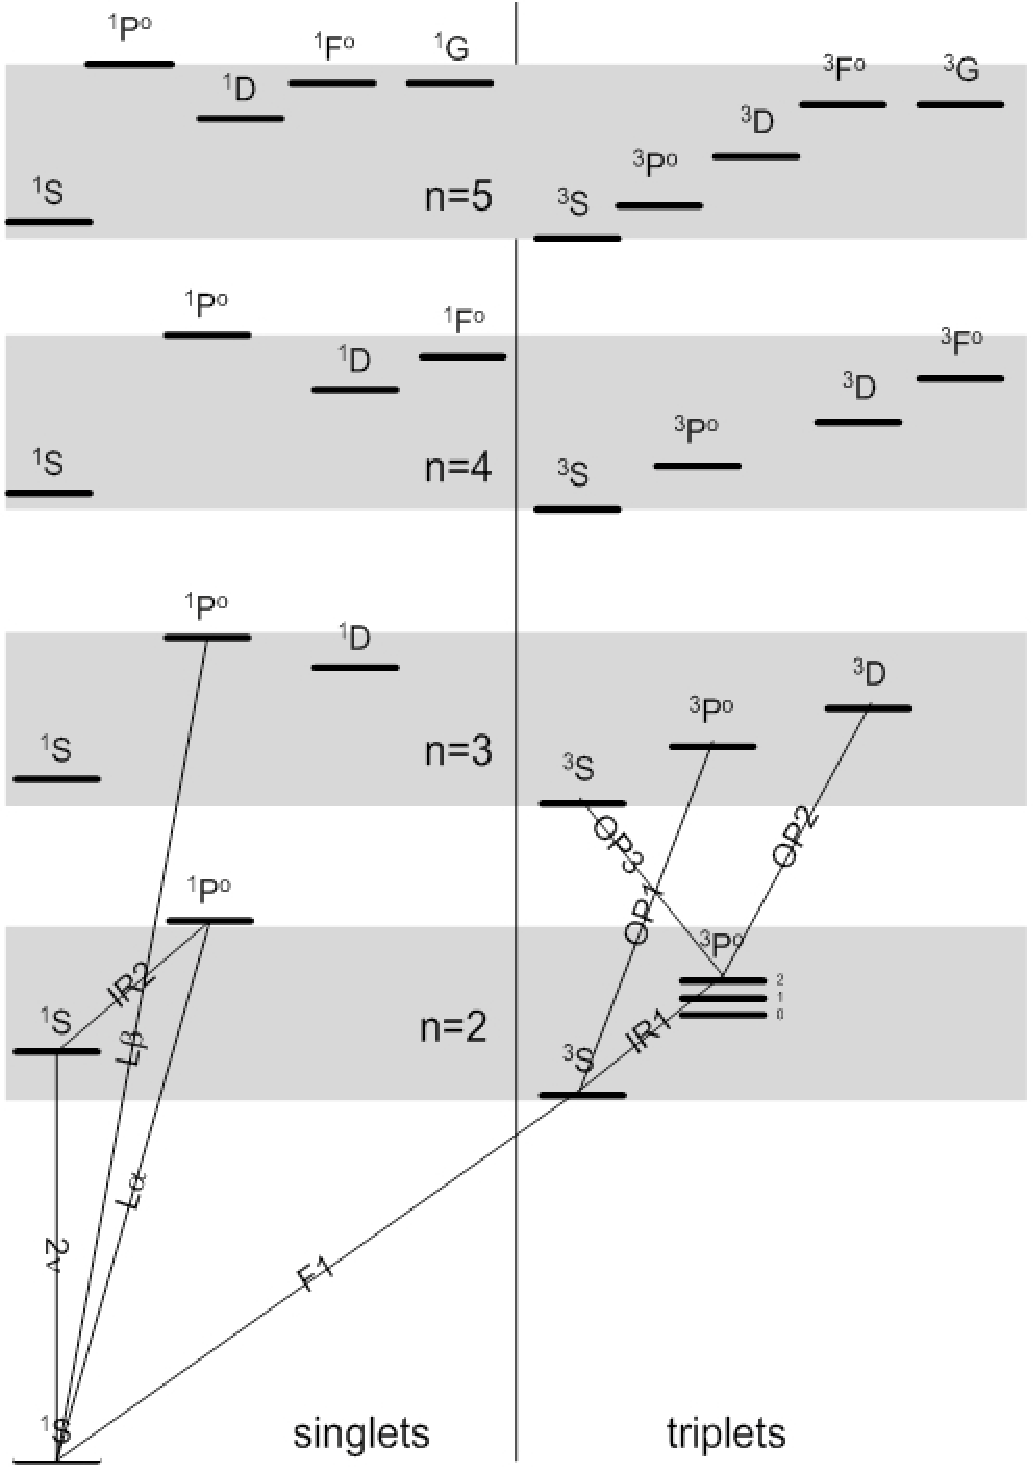
\includegraphics[scale=0.7]{helium_energy_levels}
\caption[He iso sequence energy levels]{A partial Grotrian diagram for the helium iso-electronic sequence.}
%helium
\end{figure}


Figure \ref{fig:HeEnergiesHighNLevel} compares the energies of the levels within a high-n complex
of \hei.  For comparison, the equivalent hydrogenic energies is drawn as
a dotted line.  The $^1P$ level is actually above the hydrogenic level but
all other \hei\ levels are below, and their energies approach the hydrogen
case as the angular momentum increases.  Singlets always have higher energies
than triplets.

\begin{figure}
\label{fig:HeEnergiesHighNLevel}
\centering
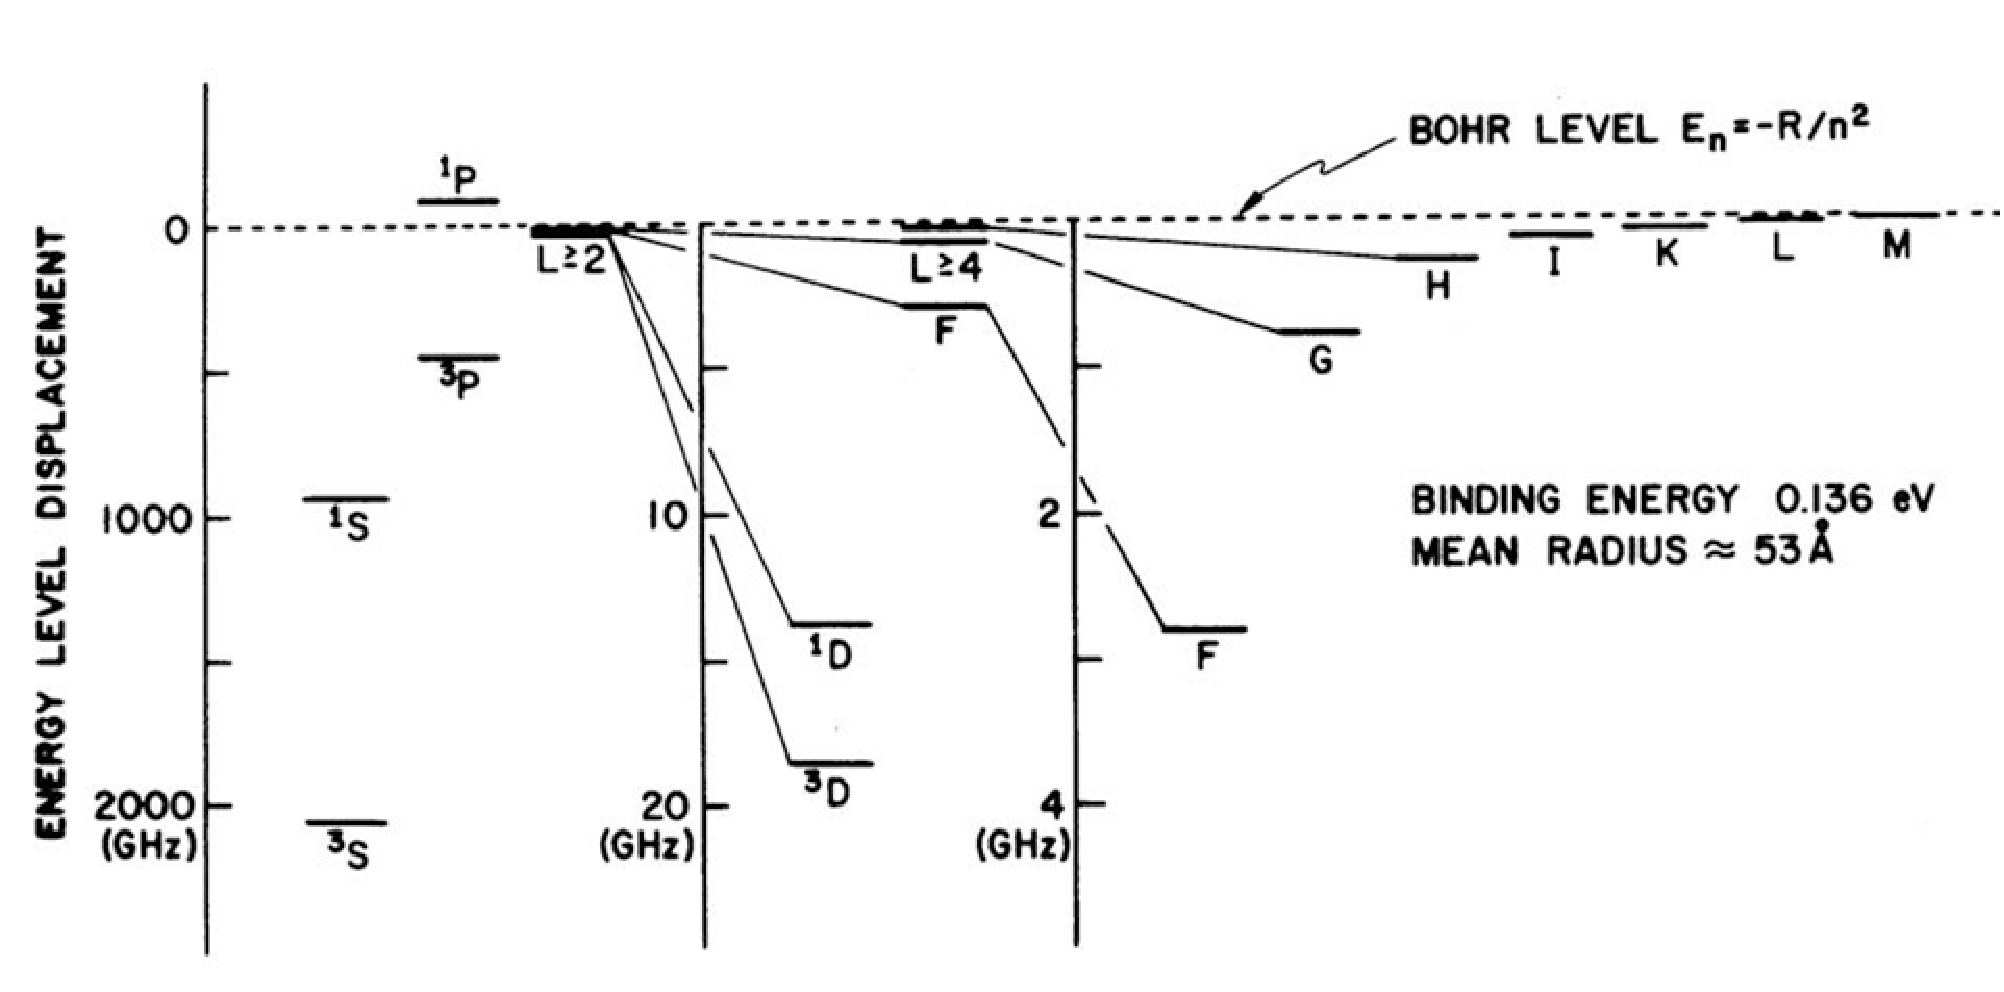
\includegraphics[scale=0.5]{HeEnergiesHighNLevel}
\caption[Energies within high-n levels of He]{A  comparison of energies of various states within a high-$n$ state
of He0.  From Wing \& McAdam (1978).}
\end{figure}

Wavelengths for lines coming from the $n = 2$ complex are listed in
Table~\ref{tab:HeLikeWavelengths}

\begin{table}
\label{tab:HeLikeWavelengths}
\caption{Wavelengths of transitions of the He-like sequence}
\begin{tabular}{lllllllll}
\hline
Z& Elem& 2 $^1$P-1 $^1$S& 2 $^3$P1-1 $^1$S& 2 $^3$P2-1 $^1$S& 2 $^3$S-1
$^1$S& 2 $^3$P$_2$-2 $^3$S& 2 $^3$P$_1$-2 $^3$S& 2 $^3$P$_0$-2 $^3$S\\
\hline
2&He& 584.3A& 591.4A& 591.4A& 625.6A& 1.083m& 1.083m& 1.083m\\
3& Li& 199.3A& 202.3A& 202.3A& 210.1A&
5484A& 5485A& 5483A\\
4& Be& 100.3A& 101.7A& 101.7A& 104.5A& 3721A& 3723A& 3721A\\
5& B&
60.31A& 61.09A& 61.09A& 62.44A& 2822A& 2826A& 2825A\\
6& C& 40.27A& 40.73A& 40.73A& 41.47A& 2271A&
2278A& 2277A\\
7& N& 28.79A& 29.08A& 29.08A& 29.53A& 1897A& 1907A& 1908A\\
8& O&
21.60A& 21.81A& 21.80A& 22.10A& 1624A& 1638A& 1640A\\
9& F& 16.81A& 16.95A& 16.94A& 17.15A& 1395A&
1414A& 1417A\\
10& Ne& 13.45A& 13.55A& 13.55A& 13.70A& 1248A& 1273A&
1278A\\
11& Na& 11.00A& 11.08A& 11.08A& 11.19A& 1112A& 1142A&
1149A\\
12& Mg& 9.169A& 9.231A& 9.228A& 9.314A& 997.5A& 1034A&
1043A\\
13& Al& 7.757A& 7.807A&7.804A& 7.872A& 899.7A& 943.2A& 954.3A\\
14& Si& 6.648A& 6.688A& 6.685A& 6.740A& 814.7A& 865.1A& 878.6A\\
15& P& 5.760A& 5.793A& 5.790A& 5.836A& 740.0A& 797.5A& 813.2A\\
16& S& 5.039A& 5.066A& 5.063A& 5.102A& 673.4A& 738.3A& 756.3A\\
17& Cl& 4.444A& 4.468A& 4.464A& 4.497A& 613.8A& 686.1A& 706.0A\\
18& Ar& 3.949A& 3.969A& 3.966A& 3.994A& 560.0A& 639.6A& 661.6A\\
19& K& 3.532A& 3.550A& 3.546A& 3.571A& 510.7A& 596.3A& 621.5A\\
20& Ca& 3.177A& 3.193A& 3.189A& 3.211A& 466.9A& 560.7A& 585.9A\\
21& Sc& 2.873A& 2.887A& 2.883A& 2.903A& 426.1A& 525.1A& 553.6A\\
22&Ti& 2.610A& 2.623A& 2.619A& 2.637A& 389.5A& 496.6A& 523.9A\\
23&V& 2.382A& 2.393A& 2.389A& 2.406A& 355.8A& 469.0A& 496.9A\\
24&Cr& 2.182A& 2.193A& 2.189A& 2.203A& 325.0A& 444.0A& 472.1A\\
25& Mn& 2.006A& 2.016A& 2.012A& 2.026A& 296.8A& 421.1A& 449.3A\\
26& Fe& 1.850A& 1.860A& 1.855A& 1.868A& 271.2A& 400.3A& 428.2A\\
27& Co& 1.712A& 1.721A& 1.716A& 1.728A& 247.6A& 381.2A& 408.6A\\
28& Ni& 1.588A& 1.597A& 1.592A& 1.604A& 226.3A& 363.9A& 390.5A\\
29& Cu& 1.478A& 1.485A& 1.481A& 1.492A& 206.7A& 347.7A& 373.5A\\
30& Zn& 1.378A& 1.385A& 1.381A& 1.391A& 188.9A& 333.0A& 357.3A\\
\hline
\end{tabular}
\end{table}


\section{The He I triplets}

   The population of the metastable 2s $^3$S level is determined including
all processes that create and destroy the level.  Processes that destroy
2s 3S include photoionization and collisional ionization, radiative decays
to ground, and collisional transitions to the singlets.  Processes that
create populations include three-body and radiative recombination and
collisions to the triplets from the singlets.  Including only radiative
recombination, exchange collisions to the singlets, and radiative decays
to ground, the relative population of the 2$^3$S level of He$^0$ can be written
as
\begin{equation}
\frac{{He({2^3}S)}}{{H{e^ + }}} = \frac{{5.79 \times {{10}^{ - 6}}\;t_4^{
- 1.18}}}{{1 + 3110\,t_4^{ - 0.51}n_e^{ - 1}}}
\end{equation}
where $t_4$ is the electron temperature in units of 10$^4$~K.

\section{Collapsed versus resolved levels}

A level in which all of the spin and angular momentum states are
explicitly determined individually is said to be resolved.  One in which
these are replaced by a single level, with the sublevels assumed to be
populated according to their statistical weight, is said to be collapsed.
Treating a level as a collapsed levels saves computer time and is appropriate
if the density is high enough for collisions to make the state fully l-mixed.

Figure \ref{fig:l_mixed_pengelly_seaton} shows a plot of the density needed to $l$-mix a level (the y-axis)
vs the principle quantum number (the x-axis).  The data are taken from
\citet{PengellySeaton1964}.
This can be used as a guide for adjusting what
levels can be treated as the collapsed case.

\begin{figure}
\centering
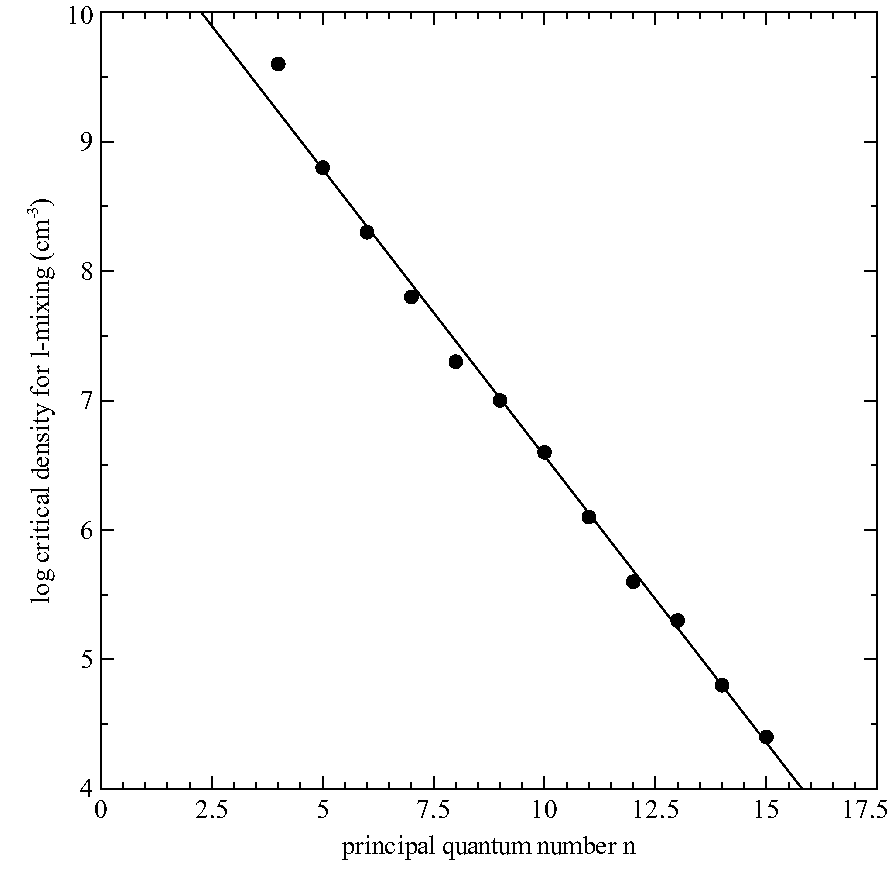
\includegraphics{l_mixed_pengelly_seaton}
\label{fig:l_mixed_pengelly_seaton}
\caption[l-mixed principle quantum number vs density]
{The lowest principle quantum number which can be treated as $l$-mixed
(the x-axis) is shown versus the density for this to occur (the y-axis).
Original data taken from \citet{PengellySeaton1964}.}
\end{figure}

\section{Emission from a pure helium gas}

Figure \ref{fig:HeI_emission} shows the predicted line and continuous
emission for a pure helium gas.

\begin{figure}
\label{fig:HeI_emission}
\centering
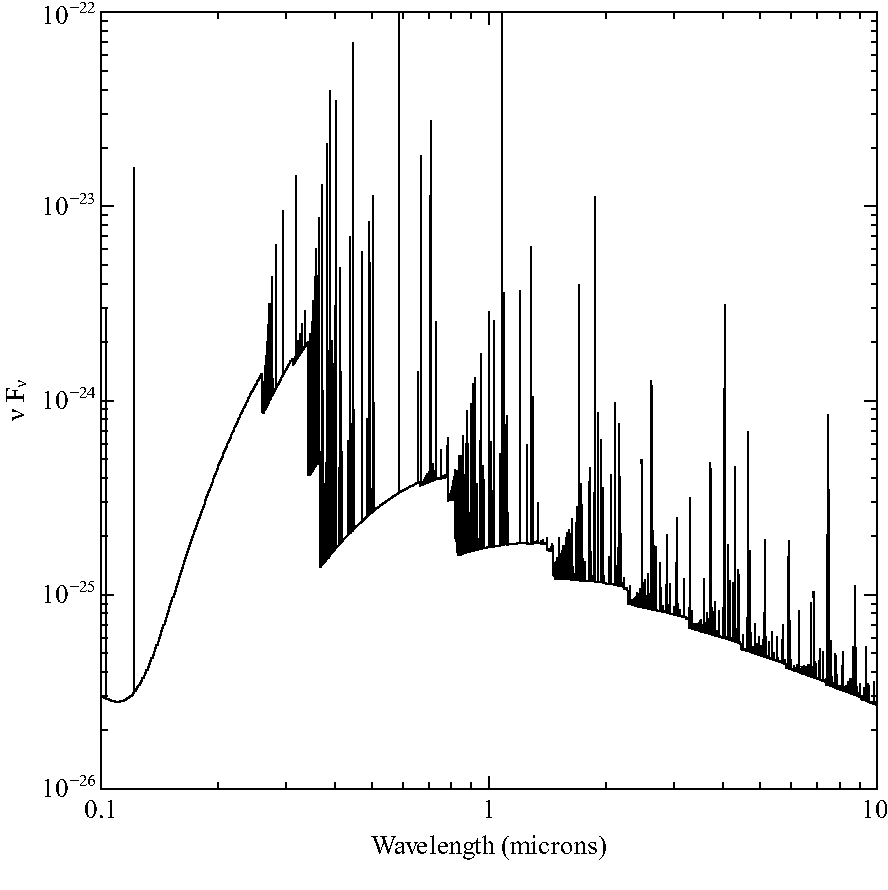
\includegraphics{HeI_emission}
\caption[He I emission]
{The net emission from a pure atomic helium gas at $10^4 \K$.  This
is from the calculation \cdFilename{heatomt10.in}
in the test suite.}
\end{figure}
%proof 1
\chapter{\hminus\ AND MOLECULES}
% !TEX root = hazy3.tex

\section{Overview}

An ion-molecule network, initially based on \citet{Black1978} but heavily
revised to include a large network, is included in \Cloudy.  Aspects are
discussed in \citet{Ferland1989}, \citet{Ferland1994},
\citet{FerlandFabian2002}, \citet{Henney2005}, and \citet{Abel2005}.
\citet{Roellig2007} present
the results of a workshop that compared various codes' predictions of
conditions in atomic and molecular clouds.

\section{The Saha equation for arbitrary systems}

The Boltzmann equation relates the densities of related species by the
expression
\begin{equation}
\label{eqn:BoltzmannPopulations}
\frac{{{n_{final}}}}{{{n_{initial}}}} = \frac{{{\rho _{final}}}}{{{\rho
_{initial}}}}\exp \left( { - \Delta E/kT} \right)
\end{equation}
where $n_{initial}$  and $n_{final}$  indicate the densities of the initial and final
states, and the $\rho$'s are the densities of available states at a given energy.
Consider the process $i \Rightarrow j+k$.  The energy change during this process is
\begin{equation}
\Delta E = {\chi _I} + \frac{1}{2}m{v^2}
\end{equation}
where the first term is the ionization or dissociation potential of the
initial system, and the second term represents the kinetic energy of the
system in the final state.  The sign of $\Delta E$ is related to the energies of
the initial and final systems~by
\begin{equation}
{E_{final}} = {E_{initial}} + \Delta E.
\end{equation}
The $\rho$'s entering equation 1 are the total densities of states accessible
at an energy $E$.  Since the initial state is a bound particle we can take
it as at rest in the lab frame, and consider the final state consisting
of two constituent particles moving with kinetic energy $\Delta$E.  The density
of states of the final particles can be written as the product of densities
of states due to electron spin and to motion of the particle.  Nuclear spins
are assumed to be uncorrelated, so nuclear statistical weights cancel out
and are not carried through.

Considering only spin and motion (momentum) the total density of states
is the spin statistical weight of the particle $g_{spin}$ multiplied by the
density of states due to momentum $g_p$ (\citealp{Mihalas1978}, p 112; \citealp{Elitzur1992},
p 14):
\begin{equation}
{\rho _{total}} = {g_{spin}}{g_p}
\end{equation}
where $g_p$ is
\begin{equation}
{g_p} = \frac{{dx\,dy\,dz\,d{p_x}\,d{p_y}\,d{p_z}}}{{{h^3}}}.
\end{equation}
The volume element can be removed from the problem by defining it as the
volume containing one particle,
\begin{equation}
dx\,dy\,dz = {\left( {{n_k}/{g_k}} \right)^{ - 1}}
\end{equation}
while the momentum volume element is given in terms of the particle's speed
$u$ by
\begin{equation}
\label{eqn:MomentumVolume}
d{p_x}\,d{p_y}\,d{p_z} = 4\pi {p^2}\,dp = 4\pi \,{m^3}{u^2}\,du.
\end{equation}
Combining these with equation \ref{eqn:BoltzmannPopulations} we find
\begin{equation}
\frac{{{n_{final}}{n_k}}}{{{n_{initial}}}} = \frac{{{n_j}{n_k}}}{{{n_i}}}
= \left( {\frac{{{g_{spin,j}}{g_{spin,k}}}}{{{g_{spin,i}}}}} \right)\left(
{\frac{{{g_{p,j}}{g_{p,k}}}}{{{g_{p,i}}}}} \right)\exp \left( { - \Delta
E/kT} \right).
\end{equation}
Shortening $g_{spin,x}$ to simply $g_x$, and using equation \ref{eqn:MomentumVolume}, we find
\begin{equation}
\frac{{{n_j}{n_k}}}{{{n_i}}} = \left( {\frac{{{g_j}{g_k}}}{{{g_i}}}}
\right)\left( {\frac{{4\pi }}{{{h^3}}}\frac{{m_j^3u_j^2{\kern 1pt} \exp
\left( { - \frac{1}{2}{m_j}u_j^2/kT} \right)d{u_j}\,m_k^3u_k^2
\exp \left( { - \frac{1}{2}{m_k}u_k^2/kT} \right)d{u_k}}}{{\,m_i^3u_i^2 \exp \left( { - \frac{1}{2}{m_i}u_i^2/kT} \right)d{u_i}}}} \right)\exp \left( { - \Delta E/kT} \right)
\end{equation}
Integrating each energy term over velocity, making the substitution
\begin{equation}
x \equiv {\left( {\frac{m}{{2kT}}} \right)^{1/2}}u,
\end{equation}
we find
\begin{equation}
\int_0^\infty  {u_j^2{\kern 1pt} \exp \left( { - \frac{1}{2}{m_j}u_j^2/kT}
\right)d{u_j}{\kern 1pt} }  = {\left( {\frac{{2kT}}{{{m_j}}}}
\right)^{3/2}}\int_0^\infty  {\exp \left( { - {x^2}} \right){x^2}\,dx}
= {\left( {\frac{{2kT}}{{{m_j}}}} \right)^{3/2}}\frac{{{\pi ^{1/2}}}}{4}
\end{equation}
where the root $\pi$ over 4 is the value of the integral.  The final form of
the Saha equation, for an arbitrary system, is:
\begin{equation}
\begin{array}{ccc}
 \frac{{{n_j}{n_k}}}{{{n_i}}}& =& \left( {\frac{{{g_j}{g_k}}}{{{g_i}}}}
\right){\left( {\frac{{2\pi \,kT}}{{{h^2}}}\frac{{{m_j}{m_k}}}{{{m_i}}}}
\right)^{3/2}}\exp \left( { - \Delta E/kT} \right) \\
&=& 8.7819 \times {10^{55}}\left( {\frac{{{g_j}{g_k}}}{{{g_i}}}}
\right){\left( {\frac{{T{m_j}{m_k}}}{{{m_i}}}} \right)^{3/2}}\exp \left(
{ - \Delta E/kT} \right) \\
 \end{array}.
\end{equation}
For the case of ionization producing an electron, the mass of the electron
is neglected relative to the mass of the atom.  If the atom and ion are
$i$ and $j$, then we have a mass ratio factor that is basically
\begin{equation}
\frac{{{m_j}{m_k}}}{{{m_i}}} = \frac{{{m_{ion}}{m_e}}}{{{m_{atom}}}}
\approx {m_e}.
\end{equation}
The most common final expression (\citealp{Mihalas1978}) includes the assumption
that $m_i$ and $m_k$ are nearly identical, and cancel out.   In this case we obtain
the form of the Saha equation most often encountered for hot gas, with the
2 being the spin statistical weight of the electron:
\begin{equation}
\frac{{{n_{ion}}{n_e}}}{{{n_{atom}}}} = \left(
{\frac{{{g_{ion}}2}}{{{g_{atom}}}}} \right){\left( {\frac{{2\pi
\,{m_e}kT}}{{{h^2}}}} \right)^{3/2}}\exp \left( { - \Delta E/kT} \right).
\end{equation}
In the case of molecular hydrogen
\begin{equation}
\frac{{{n_{\mathrm{H}}}{n_{\mathrm{H}}}}}{{{n_{{{\mathrm{H}}_{\mathrm{2}}}}}}} = 4{\left(
{\frac{{\pi \,kT{m_p}}}{{{h^2}}}} \right)^{3/2}}\exp \left( { - \Delta E/kT}
\right).
\end{equation}

\section{LTE Populations of hydrogen molecules}

In much of the following discussion comparison and relationships will
be made between the predicted hydrogen species populations and their LTE
values.

The statistical weight of H$_2^+$ is 4 while that of H$_2$ is 1 and the
dissociation energies are 2.647 eV and 4.477 eV respectively.

The LTE relative population density of \hminus\ is
\begin{equation}
{P^*}\left( {{{\mathrm{H}}^ - }} \right) = \frac{{{n^*}\left( {{{\mathrm{H}}^
- }} \right)}}{{{n_e}n\left( {{{\mathrm{H}}^{\mathrm{0}}}} \right)}} =
\frac{{{g_{{{\mathrm{H}}^ - }}}}}{{{g_{{{\mathrm{H}}^{\mathrm{0}}}}}{g_e}}}{\left(
{\frac{{{h^2}}}{{2\pi \,{m_e}kT}}} \right)^{3/2}}\exp \left[ {I({{\mathrm{H}}^
- })/kT} \right]\quad  [\mathrm{cm}^3]
\end{equation}
where $g_i$ is the statistical weight of the constituents,
(${g_{{{\mathrm{H}}^{\mathrm{ - }}}}} = 1$; ${g_{{{\mathrm{H}}^{\mathrm{0}}}}} = 2$; and
${g_e} = 2$),  the binding energy of the negative hydrogen ion is $I$(\hminus) = 0.055502
Ryd, and other constants have their usual meaning.

The LTE relative population density of H$_2$ is
\begin{equation}
{P^*}\left( {{{\mathrm{H}}_2}} \right) = \frac{{{n^*}\left( {{{\mathrm{H}}_2}}
\right)}}{{n\left( {{{\mathrm{H}}^{\mathrm{0}}}} \right)n\left( {{{\mathrm{H}}^{\mathrm{0}}}}
\right)}} =
\frac{{{g_{{{\mathrm{H}}_2}}}}}{{{g_{{{\mathrm{H}}^{\mathrm{0}}}}}{g_{{{\mathrm{H}}^{\mathrm{0}}}}}}}{\left(
{\frac{{{h^2}}}{{\pi \,{m_p}kT}}} \right)^{3/2}}\exp \left[
{I({{\mathrm{H}}_2})/kT} \right] [\mathrm{cm}^3]
\end{equation}

\section{The \hminus\ balance; radiative processes}

Although only a trace amount of hydrogen is in the form of \hminus, the opacity
provided by this ion is often dominant in the optical and near infrared,
and it couples energy in the near infrared continuum to moderately ionized
gas.  The methods and approximations employed to include heating and cooling
by \hminus\ are described here. Other discussions can be found in
\citet{Lambert1968}, \citet{Vernazza1981}, and \citet{Lites1984}.
This section is based on \citet{Ferland1989}.

The equilibrium density of \hminus\  is determined by assuming statistical
equilibrium, and balancing production and destruction mechanisms.  Great
care is taken in including both forward and back reactions, to ensure that
the present treatment of \hminus\ is capable of going to LTE in the limit of high
radiation or particle densities.

\subsection{Radiative attachment}

This is the most important creation mechanism for \hminus\ at low densities,
when three-body processes are negligible;
\begin{equation}
{H^o} + {e^ - } \Rightarrow {H^ - } + \gamma \quad .
\end{equation}

For temperatures greater than $10^4 \K$ the rate coefficient is evaluated
by numerically integrating the photodetachment cross section over frequency;
\begin{equation}
{\alpha _{rad}}\left( T \right) = {P^*}\left( {{{\mathrm{H}}^ - }}
\right)\int_{{\nu _o}}^\infty  {{\alpha _\nu }\frac{{8\pi \,{\nu
^2}}}{{{c^2}}}\exp \left( { - h\nu /kT} \right)\;d\nu }\quad  [\mathrm{cm}^3
\mathrm{s}^{-1}]
\end{equation}
where cross sections computed by \citet{Wishart1979} and spline interpolation
are used.  These cross sections are in excellent agreement with the velocity
operator bound-free cross sections tabulated by \citet{Doughty1966}.
The energy interval between the photodetachment threshold at 0.055502 Ryd
and $\sim$1.8 Ryd is divided into a large number of cells with logarithmically
increasing width, and the integration is carried out as a straight forward
sum.

This method is not numerically expedient for very low temperatures, where
the energy bandwidth of the integral is small, and a much finer frequency
grid would be required.  Rather, the integration was carried out using spline
interpolation and 32 point gaussian quadrature, integrating over factors
of two in $h\nu/kT$.  The results were then fitted with a set of power-laws.
The rate coefficients can be approximated by:
\begin{equation}
\alpha(T)_e)=\left\{\begin{array}{lc}
8.934 \times 10^{18}T^{0.505}& 1K\le T < 31.62 K\\
5.159 \times 10^{18}T^{0.664}& 31.62K\le T < 90 K\\
2.042 \times 10^{18}T^{0.870}& 90K\le T < 1200 K\\
8.861 \times 10^{18}T^{0.663}& 1200K\le T < 3800 K\\
8.204 \times 10^{17}T^{0.303}& 3800K\le T < 10^4 K\\
\end{array}\right.\quad [\mathrm{cm}^3\; \mathrm{s}^{-1}]
\end{equation}
These approximations fit the exact numerical results with a mean deviation
of 0.7 percent, and the largest error of 2.05 percent, over the indicated
temperature range.

Tests show that the numerical radiative attachment rates computed here
are in very good agreement with the approximation given by \citet{Hutchings1976},
who used the cross sections computed by \citet{Doughty1966}, for
temperatures $500 \K \le T  \le 2500 \K$.  (Notice that there is a typographical error
in the approximation for the radiative attachment rate given by
\citet{Palla1983}.)  It is also within 10\% of the value given
by \citet{Dalgarno1963}, which was based on earlier calculations
of the photodetachment cross section.

Continuum occupation numbers can be large in the infrared.  The induced
radiative attachment rate coefficient is
\begin{equation}
{\alpha _{ind}}(T) = {P^*}({{\mathrm{H}}^ - })\int_{{\nu _o}}^\infty  {{\alpha
_\nu }\frac{{4\pi \,{J_\nu }(\tau )}}{{h\nu }}} \exp \left( { - h\nu /kT}
\right)\;d\nu \quad [\mathrm{cm}3 \mathrm{s}^{-1}]
\end{equation}
where the mean intensity of the depth-dependent continuum is $J_{\nu}(\tau)$.  This
expression is used for all temperatures.

\subsection{Photodetachment}

Photodetachment,
\begin{equation}
{{\mathrm{H}}^ - } + \gamma  \Rightarrow {{\mathrm{H}}^{\mathrm{0}}} + {e^ - },
\end{equation}
is the dominant \hminus\ destruction mechanism for many conditions.  The rate
is evaluated in the standard manner;
\begin{equation}
\Gamma \left( {{{\mathrm{H}}^ - }} \right) = \int_{{\nu _o}}^\infty  {{\alpha
_\nu }\left( {bf} \right)\frac{{4\pi \,{J_\nu }(\tau )}}{{h\nu }}} \;d\nu
\quad [\mathrm{s}^{-1}]
\end{equation}
The integral is evaluated as a sum over the numerically binned continuum.
The incident continuum is then attenuated by optical depth increments
\begin{equation}
d\tau ({{\mathrm{H}}^ - }) = {\alpha _\nu }(bf)\;n({{\mathrm{H}}^ - })\left\{
{1 - \exp \left( { - h\nu /kT} \right)/{b_{{{\mathrm{H}}^ - }}}}
\right\}\;f(r)\;dr
\end{equation}
where ${b_{\mathrm{H}^ - }}$
 is the departure coefficient for \hminus, ${b_{\mathrm{H}}^{ - }}$
$\equiv  n(\mathrm{H}^-)/n^*(\mathrm{H}^-), f(r)$ is the filling factor, and
$n^*$(\hminus) is the LTE \hminus\ density.

\subsection{Photodetachment by hard photons}

The \hminus\ photoabsorption cross section increases above  $\sim$3/4 Ryd, energies
where excitation of $n\ge  2$ levels is possible.  Cross sections that include
this process are taken from \citet{Broad1976}.  These calculations
do not extend to high energies, so I scaled high-energy hydrogen cross
sections by the ratio of \hminus\ to H$^o$ cross sections at 18\AA  in order to take
absorption of x- and $\gamma$- rays into account.

The cross section for ($\gamma$,2e$^-$) absorption is much smaller than
($\gamma$, e$^-$) \citep{Broad1976}, and this latter process is neglected.

\subsection{The approach to LTE; high radiation densities}

As a test of the assumptions and methods, the approach to LTE under
conditions determined by radiative attachment (spontaneous and induced)
and photodetachment are first considered.  Tests in which gas with
temperature $T$ is exposed to black body radiation fields with color
temperature $T_{color}$ are computed.  The color and gas temperatures are set
equal, $T = T_{color}$, and the intensity of the radiation field is varied up
to the black body limit.  The intensity of the radiation field is
parameterized by the equivalent energy density temperature $T_u =
(u/a)^{1/4}$,
where $u$ is the energy density (erg cm$^{-3}$; see above) and $a$ is the Stefan's
radiation density constant.  The equilibrium population of H- was computed,
including all process mentioned below, but with the hydrogen density small
enough (typically  10$^5$~cm$^{-3}$) for radiative processes to be most important.
The \hminus\ population is expressed as a departure coefficient, and the results
are shown in Figure \ref{fig:Hmi_vs_U}, for tests in which $T_{color} = 0.5, 1$, and
$2\times 10^4$~K.

\begin{figure}
\centering
\label{fig:Hmi_vs_U}
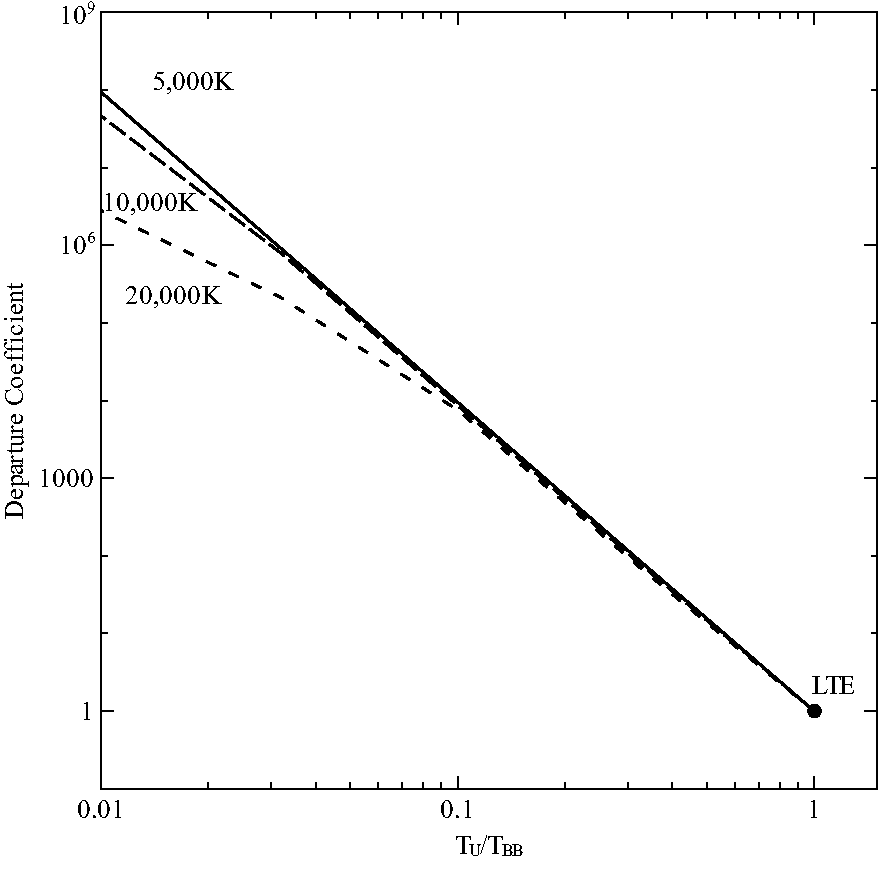
\includegraphics[scale=0.7]{Hmi_vs_U}
\caption[\protect\hminus\ departure coefficients vs radiation energy density]{Departure coefficients for \hminus.  The figure shows tests in which
the hydrogen density was held fixed at a low and the gas irradiated by black
bodies with color temperatures of 5, 10, and $20 \times 10^3$ K.  Gas temperature
and color temperatures were equal. The energy density temperature $T_u$. was
varied up to its LTE limit.  The \hminus\ departure coefficient is within 0.2\%
of unity when $T_u = T_{color}$.}
\end{figure}

When $T_u = T_{color}$, and the radiation field is in strict thermodynamic
equilibrium, radiative processes must hold \hminus\ in LTE and departure
coefficients of unity are expected.  The computed departure coefficients
for the three temperatures are 0.9998, 0.9996, and 1.0030, respectively.
As the Figure shows, when $T_u$ is lowered below $T_{color}$, the intensity of the
radiation field falls below its thermodynamic equilibrium value, and the
population of \hminus\ increases.  This is because the photodetachment rate (which
is proportional to the intensity of the radiation field) is no longer in
balance with the radiative attachment rate (which is proportional only to
the electron density).

\section{The \hminus\ balance; collisional processes}

\subsection{Associative detachment}

The most important H$_2$ formation mechanism in grain-free environments,
and a significant \hminus\ destruction mechanism, is associative detachment,
\begin{equation}
{{\mathrm{H}}^ - } + {{\mathrm{H}}^0} \Leftrightarrow {{\mathrm{H}}_2} + {e^ - }
\end{equation}
where rate coefficients were originally from Bieniek and Dalgarno (1979)
and have been updated to \citet{Launay1991}.  The rate is shown in Figure
\ref{fig:hminus_to_h2}.  The reverse reaction rate $C_R$, for electron collisional dissociation
of H$_2$, is related to the forward rate coefficient $C_F$ by detailed balance;
\begin{equation}
{C_R} = {C_F}\frac{{{P^*}({{\mathrm{H}}^ - })}}{{{P^*}({{\mathrm{H}}_2})}}
\quad  [\mathrm{s}^{-1}].
\end{equation}

\begin{figure}
\centering
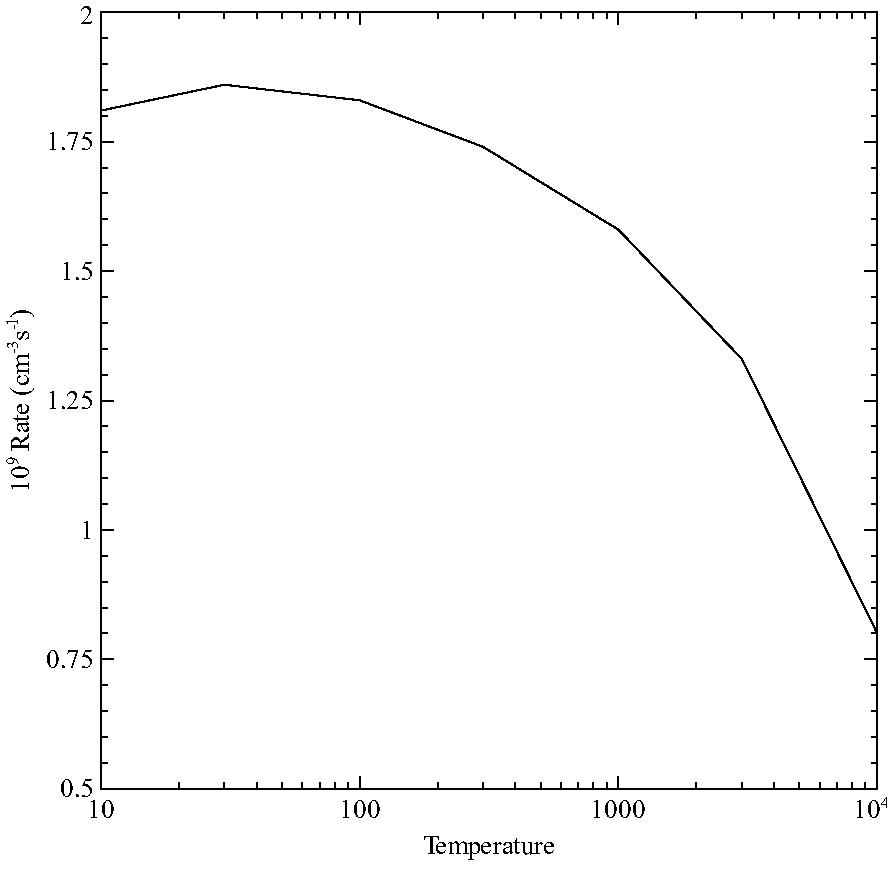
\includegraphics[scale=0.8]{hminus_to_h2}
\caption{Rate coefficient for H$^- \to \mathrm{H}_2$.
The rates are taken from Launay et al. (1991)}
\label{fig:hminus_to_h2}
\end{figure}

\subsection{Electron collisional detachment}

For nebular temperatures ($\sim10^4$~K) and moderate levels of ionization,
the process
\begin{equation}
{{\mathrm{H}}^ - } + {e^ - } \Leftrightarrow {{\mathrm{H}}^0} + 2{e^ - }
\end{equation}
is a competitive \hminus\ destruction mechanism.  Rates taken from the compendium
of \citet{Janev1987} are used.  The reverse process, electron three-body
recombination with neutral hydrogen, is included via detailed balance;
\begin{equation}
{C_R} = {C_F}\;\frac{{{P^*}({{\mathrm{H}}^ - })}}{{{P^*}({{\mathrm{H}}^0})}}
\quad [\mathrm{s}^{-1}]
\end{equation}

\subsection{Collisional ionization by suprathermal electrons}

The total suprathermal collisional ionization rate is computed using
approximations from \citet{Shull1985}.  Ionization of \hminus\ by
suprathermal electrons is scaled from the Ho rates using cross sections
at 20 eV given by \citet{Janev1987}.  This energy was chosen as
representative of the mean energy of the secondary electron shower.  The
majority of these collisions are of the form e$^- + \mathrm{H}^- \mathrm{H}(1s) +
2\mathrm{e}^-$, although
e$^- + \mathrm{H}^-  \mathrm{H}^+ + 3\mathrm{e}^-$ collisions occur roughly 1\% of the time.

\subsection{Mutual neutralization}

Neutral hydrogen can charge transfer with the negative ion through
\begin{equation}
{{\mathrm{H}}^ - } + {{\mathrm{H}}^ + } \Leftrightarrow {\mathrm{H}} +
{{\mathrm{H}}^*}\quad .
\end{equation}
The rate coefficients given in \citet{Janev1987} are used.  By far the
largest rate coefficients are for collisions that populate hydrogen in the
$n=3$ level.  These rates are based on both experimental and theoretical data
(see, for example, \citet{Peart1985}.

The reverse reaction is included using detailed balance.  If the rate
coefficient for the forward reaction is $C_F$ then the reverse reaction rate,
and its rate coefficient $C_R$, are given by
\begin{equation}
{C_F}{P^*}({{\mathrm{H}}^ - }){P^*}({{\mathrm{H}}^ + }) =
{C_R}\;{P^*}({{\mathrm{H}}^0}){P^*}({{\mathrm{H}}^0})
\end{equation}
where $n_i$ and $b_i$ are the population and departure coefficient of hydrogen
in the $i$th level.

\subsection{Charge neutralization with heavy elements}

The process
\begin{equation}
{{\mathrm{H}}^ - } + {A^ + } \Leftrightarrow {{\mathrm{H}}^{\mathrm{0}}} +
{{\mathrm{A}}^{\mathrm{0}}}
\end{equation}
is considered by \citet{Dalgarno1973}, who give rate coefficients
for very low temperatures and ionization levels.  Judging from the curves
given by \citet{Peterson1971}, upon which the \citet{Dalgarno1973} rates
are based, the approximation they give should still be valid (although very
uncertain) at temperatures of general interest ($\sim 0.5 - 1.0 \times
10^4$~K).  Here
A$^+$ is all singly ionized species, which are assumed to be neutralized at
the same rate.

\subsection{Neglected processes}

Collisional detachment by protons ($p^+ + \mathrm{H}^- \to \mathrm{H} +p^+ + e^-$), which has a
negligible rate coefficient according to \citet{Janev1987}, is neglected,
as is collisional detachment by atomic hydrogen (H$^- + \mathrm{H} \to 2\mathrm{H}
+ e^-$), which
has no reliable rate coefficient according to
\citet{Lites1984}.

\subsection{The approach to LTE; high hydrogen densities}

A series of models in collisional equilibrium was computed.  Radiative
processes were also included, but the incident radiation field, a 10$^4$~K
blackbody, was given a negligible intensity (an ionization parameter of
10$^{-12}$).  Three temperatures, 0.5, 1, and $2 \times 10^4$~K, were considered to span
the temperature range typical of regions with significant \hminus\ population.
The hydrogen density was varied between 10$^8$ and 10$^{18}$ cm$^{-3}$ to confirm the
approach to LTE at high densities.  The results of these calculations are
shown in Figure~\ref{fig:Hmi_vs_density}.

\begin{figure}
\centering
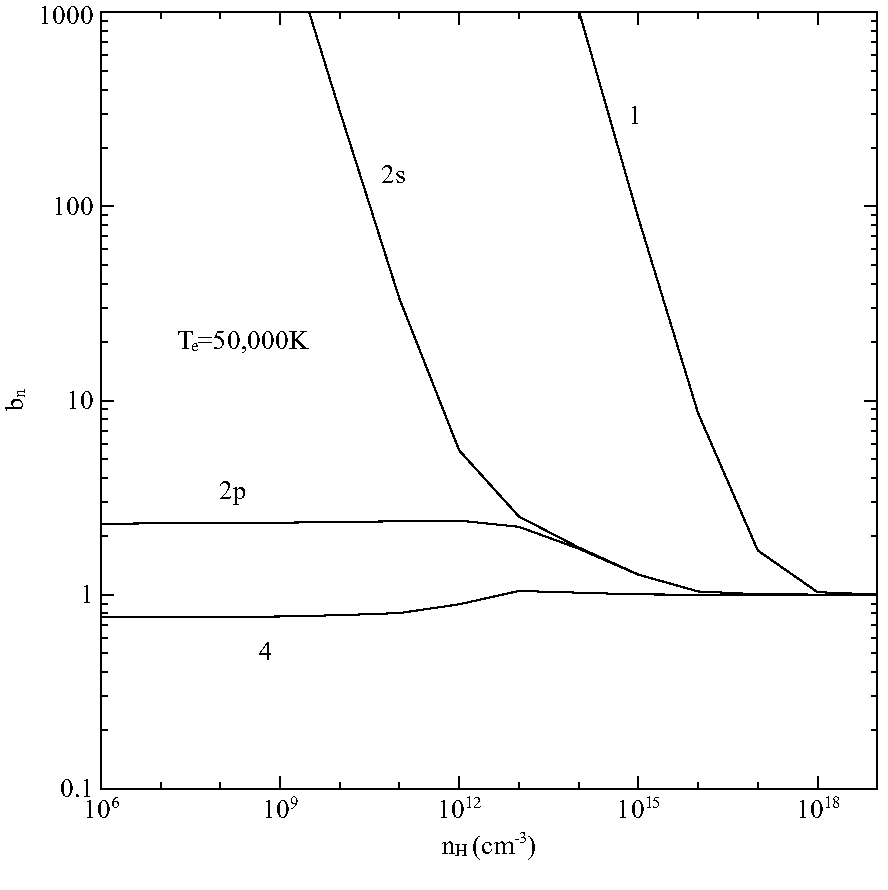
\includegraphics[scale=0.8]{Hmi_vs_density}
\caption[\protect\hminus\ departure coefficients vs density]{Departure coefficients for \hminus\ are shown. The radiation density
was low and the total hydrogen density varied.  Three gas temperatures are
shown.  Collisions bring \hminus\ to LTE at high densities.}
\label{fig:Hmi_vs_density}
\end{figure}

For the majority of the calculations hydrogen is largely neutral, and
for the smaller temperatures a significant fraction of the hydrogen was
in the molecular form (H$_2$ and H$_2^+$).  The calculation confirms that the
departure coefficients are within 2\% of unity at the highest densities
computed.

\section{The HeH$^+$ molecular ion }

Rates for radiative association of He and H$^+$ to form HeH$^+$ are taken from \citet{Zygelman1990}.

\section{Linearization of the balance equations}

In the case of a molecular balance equation it is common to have a single
reaction that is the product of two unknowns.  The code works by complete
linearization, and uses the following scheme to produce a linear chemical
network.

Suppose we have two molecules with abundance $a$ and $b$, and with previous
abundances $a_o$ and $b_o$.  Then $\delta a = a - {a_o};\;\delta b = b -
{b_o}$ and the cross terms, $ab$, can be written as
\begin{equation}
\begin{array}{ccc}
 ab& =& \left( {{a_o} + \delta a} \right)\left( {{b_o} + \delta b} \right) \\
&\approx& {a_o}\delta b + {b_o}\delta a + {a_o}{b_o} \\
&\approx& {a_o}\left( {b - {b_o}} \right) + {b_o}\left( {a - {a_o}} \right)
+ {a_o}{b_o} \\
& =& {a_o}b + a{b_o} - {a_o}{b_o} \\
 \end{array}
\end{equation}

\section{The H$_2$ molecule}

The treatment of the hydrogen is described in \citet{Shaw2005}.  Other
details are in \citet{Ferland1989},
\citet{Ferland1994}, \citet{FerlandFabian2002}, and \citet{Abel2005}, while \citet{Roellig2007} compare
predictions of various codes.

\subsection{Stoichiometry}

The time dependent form of a reaction can be written as
\begin{equation}
\frac{{\partial {n_i}}}{{\partial t}} = {n_j}{R_f} - {n_i}{R_d}
\end{equation}
where $R_f$ is the rate that species with density $n_i$ is created from a species
with density $n_j$, and $R_d$ is the rate that $n_i$ is destroyed.  In the case of
hydrogen in the interstellar medium, the dominant formation process is
catalysis on grain surfaces, and the dominant destruction process is
photodissociation by the Solomon process.  This reaction corresponds to
the process $2n\left( {{{\mathrm{H}}^0}} \right) \to n\left( {{{\mathrm{H}}_2}}
\right)$
 and H$^0$ is removed from the gas at twice the rate that H$_2$ is formed.  The
balance equation is
\begin{equation}
\label{eqn:H2FormationBlance}
\frac{{\partial {n_i}}}{{\partial t}} = \frac{1}{2}n\left( {{{\mathrm{H}}^0}}
\right)n\left( {{{\mathrm{H}}^0}} \right){R_f} - n\left( {{{\mathrm{H}}_2}}
\right){R_d}.
\end{equation}

The convention in physical chemistry is to include only microphysical
processes in a reaction rate coefficient $R$, and to explicitly write the
stoichiometric factors in the equation, as done in equation \ref{eqn:H2FormationBlance}.

Tragically, the convention is astrophysics is to write the balance
equation as $n\left( {{{\mathrm{H}}^0}} \right)n\left( {{{\mathrm{H}}^0}}
\right){R_f} = n\left( {{{\mathrm{H}}_2}} \right){R_d}$
and absorb the stoichiometric factor of $\frac{1}{2}$ into the rate
coefficient.  So, the standard or \citet{Jura1974}, \citet{Jura1975} rate of H$_2$ formation
of grain surfaces, $3\times 10^{-17}$~cm$^3$~s$^{-1}$ at 100 K, includes a stoichiometric factor
of $\frac{1}{2}$.

\subsection{Associative detachment of \hminus}

The process
\begin{equation}
{{\mathrm{H}}^ - } + {\mathrm{H}} \Rightarrow {{\mathrm{H}}_2} + e
\end{equation}
is the main H$_2$ formation mechanism in low-density grain-free regions, and
is treated as described above.
At temperatures of interest here $(\sim 10^3 \K$)
the rate for H$_2$ formation by this process is set by the rate for radiative
association to form \hminus, and is of order 10$^{-15}$ cm$^3$ s$^{-1}$ (see above).

\subsection{Catalysis on grain surfaces}

The process
\begin{equation}
2{\mathrm{H}} + {\mathrm{grain}} \Rightarrow {{\mathrm{H}}_2} + {\mathrm{grain}}
\end{equation}
is a competitive H$_2$ formation process when grains are present.  The rate
coefficient is taken from \citet{Hollenbach1979} and \citet{Cazaux2002}.  Defining the fraction of atoms which form molecules as
\begin{equation}
{f_a} = {\left( {1 + {{10}^4}\exp \left( { - 600/{T_{gr}}} \right)}
\right)^{ - 1}}
\end{equation}
then the rate coefficient is given by
\begin{equation}
{\alpha _{gr}}\left( {{{\mathrm{H}}_2}} \right) = 3 \times {10^{ -
18}}\frac{{\sqrt T {A_{gr}}\,{f_a}}}{{1 + 0.04\sqrt {{T_{gr}} + T}  + 0.002T
+ 8 \times {{10}^{ - 6}}T_{}^2}}\quad
[\mathrm{cm}^3 \mathrm{s}^{-1}]
\end{equation}
where $A_{gr}$ is the grain abundance relative to the ISM value, and $T$
and $T_{gr}$
are the electron and grain temperatures respectively.  The grain temperature
is determined self-consistently, including radiative and collisional heating
and cooling, as described in the section \cdSectionTitle{Grain Physics}.

At $T=10^3 \K$ and $T_{gr}=100 \K$ (representative values of the gas and grain
temperature in regions near a H$^0 - \mathrm{H}_2$ interface) the rate coefficient for
grain catalysis is $\sim 4\times 10^{-18}$~cm$^{-3}$~s$^{-1}$.  For most conditions where
carbon is at least once ionized radiative association through \hminus\ is at least
a competitive H$^2$ formation mechanism.  The ratio of the two processes
(referred to as the \hminus\ and grain H$_2$ formation routes) is then
\begin{equation}
\frac{{r\left( {{{\mathrm{H}}^ - }} \right)}}{{r\left( {{\mathrm{grain}}} \right)}}
= \frac{{{n_e}\alpha \left( {{{\mathrm{H}}^ - }} \right)}}{{{n_H}\alpha \left(
{{\mathrm{grain}}} \right)}} \approx \frac{{{n_e}}}{{{n_H}}}250
\end{equation}
i.e., the \hminus\ route is faster for conditions of moderate ionization
($n_e/n_{\mathrm{H}}>4\times 10^{-3}$) even when grains are present.  When grains are absent (or
deficient) the \hminus\ route dominates.

\subsection{Excited atom radiative association}

Rates for the process
\begin{equation}
{\mathrm{H}}\left( {n = 2} \right) + {\mathrm{H}}\left( {n = 1} \right) \Rightarrow
{{\mathrm{H}}_2} + h\nu
\end{equation}
are taken from \citet{Latter1991}.

\subsection{Excited molecular dissociation}

Rates for the process
\begin{equation}
{{\mathrm{H}}_2}\left( {v \ge 4} \right) + {e^ - } \Rightarrow {\left(
{{\mathrm{H}}_2^ - } \right)^*} \Rightarrow {\mathrm{H}} + {{\mathrm{H}}^ - }
\end{equation}
are given in \citet{Janev1987} (their process 2.2.17), and these have been
adopted by \citet{Lenzuni1991} and \citet{Crosas1993} in their
work on high density gas.  Tests show that this process, if taken at face
value, is by far the fastest destruction mechanism for molecular hydrogen
under ISM conditions.

The process outlined by \citet{Janev1987} involves an electron capture
by H$_2$ into vibrationally excited levels ($4 \le v \le 9$).   The process is fast
at low temperatures because the energy barrier is small, and the excited
levels have large populations at laboratory densities.  The process proceeds
much more slowly at ISM densities, however, because excited levels have
populations below their LTE value.  This situation is thus similar to that
described by \citet{Dalgarno1979}.  We have modified the \citet{Janev1987} rates using the physics outlined by \citet{Dalgarno1979}.

\subsection{Collisional dissociation by H$^0$, He$^0$, and e$^-$}

The rate coefficient for the forward process, collisional dissociation
by the species S (one of H$^0$, He$^0$, or e$^-$),
\begin{equation}
{{\mathrm{H}}_2} + S \Rightarrow 2{\mathrm{H}} + S
\end{equation}
is taken from \citet{Dove1986} (dissociation by H$^0$),
\citet{Dove1987} (dissociation by He$^o$) and \citet{Janev1987} (dissociation by electrons).
These can be important destruction mechanisms only for warm regions of the
ISM because of the large binding energy of H$_2$ ($\sim$50000~K).

The reverse reactions are included via detailed balance. Three-body
formation of H$_2$ is important only for very high densities [$n\cong
10^{10}$~cm$^{-3}$].

\section{Heavy element molecules}

\subsection{Cooling}

Cooling due to collisional excitation of vibration-rotation levels of
CH, OH, and H$_2$O is treated using the scheme outlined by HM79.

Of these CO is the most important. $^{12}$CO and $^{13}$CO are treated as
multi-level rigid rotors, with the full spectrum of the ground vibration
state predicted.


%proof 1
\chapter{THE HEAVY ELEMENTS}
% !TEX root = hazy3.tex

\section{Overview}

The code considers all 465 atoms and ions of the lightest 30 elements.
The treatment of the ionization equilibrium of ions with more than two
electrons is conventional (see AGN3).  This treatment is more approximate
than that of the H and He iso-sequences because the majority of ions are
treated considering only the ground term and continuum for each ionization
stage.  In all cases, collisional ionization from ground and a net three-body
recombination coefficient are included.
Photoionization rates are modified
for induced recombination as described by equation~\ref{eqn:InducedRecombinationRateCoefficient}.
All published charge transfer rate coefficients are also included
\citep{Kingdon1996}.  Inner shell photoionization is treated using
Auger yields given by \citet{Kaastra1993}.  Photoionization cross
sections are from \citet{VernerFerlandKorista1996}.

This treatment is approximate at high densities for two reasons.  First,
net radiative recombination coefficients, which have been summed over all
levels are used.  These sums are correct only in the low-density limit.
At high densities levels can undergo collisional ionization before radiative
decays to the ground state occur.  This brings high levels into LTE, which
actually increases the recombination rate.  A second problem is that
substantial populations can build up in highly excited states when the
density and temperature are high.  When this occurs, the partition function
of the atom or ion is no longer equal to the statistical weight of the ground
state.  As a result the ionization equilibrium of the heavy elements is
approximate for very high densities $(n \gg 10^{10} \mathrm{cm}^{-3})$, with uncertainties
increasing for higher densities.  The statistical and thermal equilibrium
of high-density gas is an area of on-going research.

Many exotic line transfer effects can influence certain lines due to
coincidental line overlap.  A good general reference to a number of these
processes is the paper by \citet{Swings1940}.  All of these processes
are included in the line formation processes for those lines that are
predicted by the code.  \citet{Morton1988} and
\citet{VernerVernerFerland1996} provide a line list for UV resonance lines, and \citet{Bowen1960}'s
paper on forbidden lines remains a classic.

The effects of resonant structures often dominate collision strengths
for infrared transitions.
\citet{Oliva1996} and \citet{VanHoof2000a} stress the uncertainties these may introduce.

\section{Solar system abundances}

Figure \ref{fig:SolarSystemAbundances} plots the solar system abundances of the elements, as tabulated
by \citet{Allende2001}, \citet{Allende2002},
\citet{Holweger2001} and \citet{Grevesse1998}.
The independent variable is the abundance by number relative to a scale where
the abundance of silicon is 10$^6$.  The dependent vaariable lists the atomic number and
the chemical symbol for the element.

\begin{figure}
\centering
\label{fig:SolarSystemAbundances}
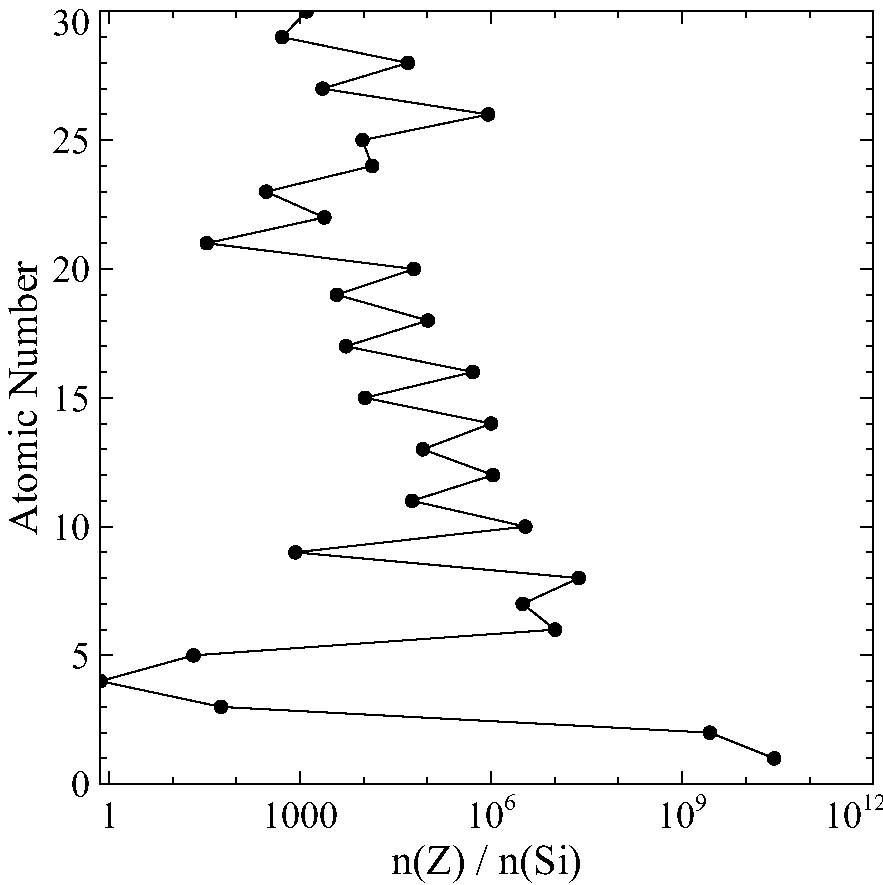
\includegraphics[scale=0.7]{SolarSystemAbundances}
\caption[Solar system abundances]{Solar system abundances are shown.}
\end{figure}

\section{Periodic table}

A periodic table of the first 36 elements follows.

\begin{center}
\begin{tabular}{lllllllllllllllllll}
\hline
1&&&&&&&&&&&&&&&&&2\\
H&&&&&&&&&&&&&&&&&He\\
3&4&&&&&&&&&&&5&6&7&8&9&10\\
Li&Be&&&&&&&&&&&B&C&N&O&F&Ne\\
11&12&&&&&&&&&&&13&14&15&16&17&18\\
Na&Mg&&&&&&&&&&&Al&Si&P&S&Cl&Ar\\
19&20&21&22&23&24&25&26&27&28&29&30&31&32&33&34&35&36\\
K&Ca&Sc&Ti&V2&Cr&Mn&Fe&Co&Ni&Cu&Zn&Ga&Ge&As&Se&Br&Kr\\
\hline
\end{tabular}
\end{center}

\section{Ionization balance}

\subsection{Photoionization cross sections}

Photoionization cross sections for all elements are evaluated using Dima
Verner's fits to Opacity Project data where possible, and the best
theoretical or experimental data for other cases.
The fitting procedure
is described in \citet{Verner1993}, \citet{Verner1995},
and \citet{VernerFerlandKorista1996}.

\subsection{Auger multi-electron ejection}

Many electrons may be ejected following removal of an inner electron.
This is fully treated using electron yields taken from
\citet{Kaastra1993}.
This process couples non-adjacent stages of ionization.

Figure \ref{fig:IronPhoto} shows photoionization cross sections for each shell of singly
ionized iron, along with plots of the electron yield, assuming data given
by \citet{Kaastra1993}.  A single photoionization of the 1s shell can
remove as many as 8 electrons.

\begin{figure}
\centering
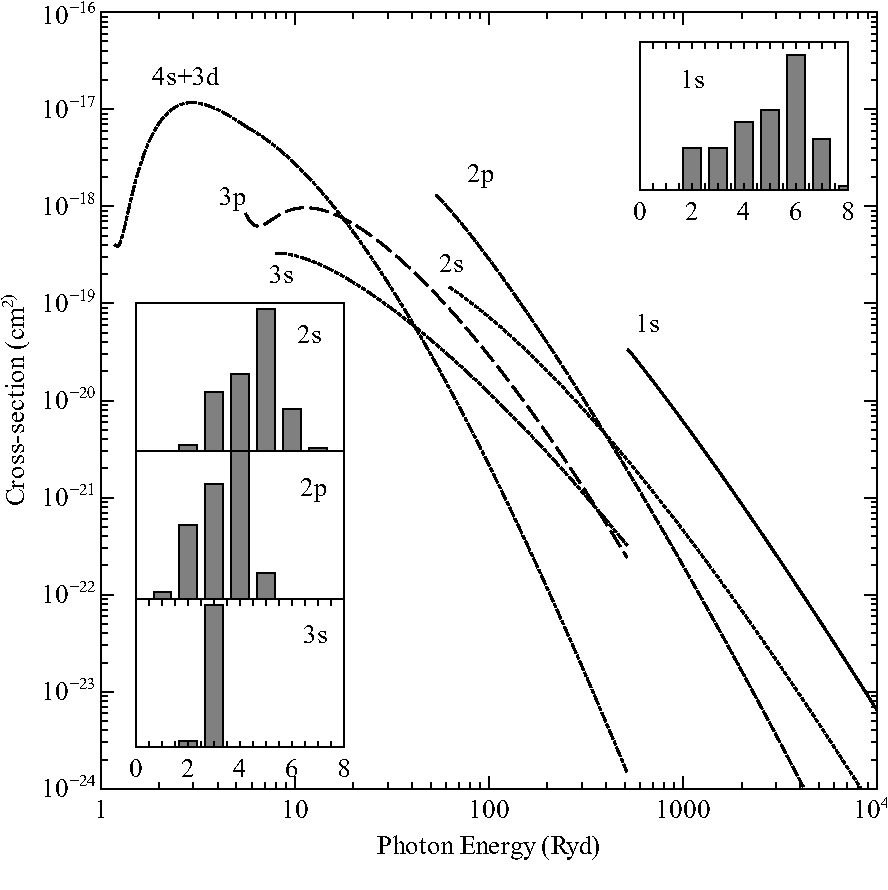
\includegraphics[scale=0.6]{IronPhoto}
\caption[Photoionization cross sections and yields for Fe$^+$]
{Photoionization cross sections and electron yields for singly
ionized iron.  Each subshell is shown along with the corresponding electron
yield.}
\label{fig:IronPhoto}
\end{figure}

\subsection{Compton scattering ionization of bound electrons}

Ionization of outer valence electrons by Compton scattering is treated
for all species by assuming that the cross section is the relativistic
Compton cross section, multiplied by the number of valence electrons.

\subsection{Collisional ionization rate coefficients}

Fits to collisional ionization rate coefficients are evaluated in Dima
Verner's routine \cdRoutine{cfit}.
These rates come mainly from \citet{Arnaud1992}
and \citet{Arnaud1985}, and by interpolation where rates
are not given.

\subsection{Charge transfer}

Rates for charge transfer between hydrogen and the heavy elements are
evaluated using Jim Kingdon's routines.   For species more than 4 times
ionized, a statistical estimate made by Alex Dalgarno (\citealp{Ferland1997})
is used.  The rate coefficient for transfer between atomic hydrogen and
a highly ionized species is given by
$1.92\times 10^{-9} \; \zeta \; \pcc \ps$,
where $\zeta$ is the
charge of the ion.  Other atoms are treated analogously.

All of these include the thermal effects of charge transfer, as described
by \citet{Kingdon1998b}.

\section{Ionization potentials}

Table \ref{tab:IonizationPotentials} lists ionization potentials for photoionization of the outer
shell of the first thirty elements.  These are given in Rydbergs for infinite
mass nuclei.

\begin{table}
\begin{center}
\scriptsize
\caption{Ionization Potentials of the Elements (Rydbergs)}
\label{tab:IonizationPotentials}
\begin{tabular}{lllllllllll}
\hline
&1 H& 2 He& 3 Li& 4 Be& 5 B& 6 C& 7 N& 8 O& 9 F& 10 Ne\\
\hline
1& 9.996(-1)& 1.807& 3.963(-1)& 6.852(-1)& 6.099(-1)& 8.276(-1)& 1.068&
1.001& 1.280& 1.585\\
2&& 4.000& 5.559&
1.338& 1.849& 1.792& 2.176& 2.581& 2.570& 3.010\\
3&&&  9.003& 1.131(+1)& 2.788& 3.520&
3.487& 4.038& 4.609& 4.664\\
4&&&&  1.600(+1)& 1.907(+1)& 4.740& 5.694& 5.689& 6.405& 7.138\\
5&&&&&  2.500(+1)& 2.882(+1)& 7.195& 8.371& 8.393& 9.275\\
6&&&&&&
3.601(+1)& 4.058(+1)& 1.015(+1)& 1.155(+1)& 1.161(+1)\\
7&&&&&&& 4.903(+1)& 5.434(+1)& 1.361(+1)& 1.524(+1)\\
8&&&&&&&& 6.405(+1)& 7.011(+1)& 1.757(+1)\\
9&&&&&&&&& 8.107(+1)& 8.790(+1)\\
10&&&&&&&&&& 1.001(+2)\\
\hline
\end{tabular}
\end{center}
\end{table}

\begin{table}
\begin{center}
\addtocounter{table}{-1}
\scriptsize
\caption{Ionization Potentials of the Elements (Rydbergs) -- Continued}
\begin{tabular}{lllllllllll}
\hline
&11 Na& 12 Mg& 13 Al& 14 Si& 15 P&16 S& 17 Cl& 18 Ar& 19 K& 20 Ca\\
\hline
1&
3.777(-1)&5.620(-1)&4.400(-1)&5.991(-1)&7.710(-1)&7.614(-1)&9.533(-1)&1.158&
3.191(-1)&4.493(-1)\\
2& 3.476& 1.105& 1.384& 1.202& 1.450& 1.715& 1.750& 2.031& 2.325&
8.724(-1)\\
3& 5.264& 5.890& 2.091& 2.461& 2.220& 2.560& 2.911& 2.994& 3.367& 3.742\\
4& 7.270&
8.033& 8.820& 3.318& 3.781& 3.477& 3.930& 4.396& 4.477& 4.944\\
5& 1.017(+1)& 1.039(+1)& 1.130(+1)& 1.226(+1)& 4.780& 5.342& 4.985& 5.514&
6.075& 6.211\\
6& 1.266(+1)& 1.371(+1)& 1.400(+1)& 1.507(+1)& 1.620(+1)& 6.471& 7.131&
6.689& 7.309& 7.996\\
7& 1.532(+1)& 1.653(+1)& 1.774(+1)& 1.812(+1)& 1.934(+1)& 2.065(+1)& 8.393&
9.136& 8.643&
9.349\\
8& 1.942(+1)& 1.955(+1)& 2.092(+1)& 2.228(+1)& 2.274(+1)& 2.412(+1)&
2.560(+1)& 1.055(+1)& 1.137(+1)& 1.082(+1)\\
9& 2.204(+1)& 2.412(+1)& 2.426(+1)& 2.580(+1)& 2.732(+1)& 2.786(+1)&
2.941(+1)& 3.105(+1)& 1.292(+1)& 1.384(+1)\\
10& 1.077(+2)& 2.701(+1)& 2.935(+1)& 2.950(+1)& 3.120(+1)& 3.286(+1)&
3.349(+1)& 3.518(+1)& 3.703(+1)& 1.553(+1)\\
11& 1.212(+2)& 1.295(+2)& 3.249(+1)& 3.499(+1)& 3.525(+1)& 3.710(+1)&
3.890(+1)& 3.961(+1)& 4.150(+1)& 4.350(+1)\\
12&& 1.443(+2)& 1.533(+2)& 3.848(+1)& 4.119(+1)& 4.150(+1)& 4.351(+1)&
4.544(+1)& 4.627(+1)& 4.830(+1)\\
13&&&  1.693(+2)& 1.792(+2)& 4.497(+1)& 4.790(+1)& 4.827(+1)& 5.043(+1)&
5.253(+1)& 5.341(+1)\\
14&&&& 1.965(+2)& 2.070(+2)& 5.198(+1)& 5.511(+1)& 5.555(+1)& 5.782(+1)&
6.010(+1)\\
15&&&&& 2.256(+2)& 2.370(+2)& 5.949(+1)& 6.283(+1)& 6.329(+1)& 6.575(+1)\\
16&&&&&& 2.568(+2)& 2.689(+2)& 6.747(+1)& 7.115(+1)& 7.162(+1)\\
17&&&&&&& 2.900(+2)& 3.029(+2)& 7.607(+1)& 7.989(+1)\\
18&&&&&&&& 3.253(+2)& 3.389(+2)& 8.504(+1)\\
19&&&&&&&&& 3.626(+2)& 3.770(+2)\\
20&&&&&&&&&& 4.020(+2)\\
\hline
\end{tabular}
\end{center}
\end{table}

%   Table 1c
\begin{table}
\begin{center}
\addtocounter{table}{-1}
\scriptsize
\caption{Ionization Potentials of the Elements (Rydbergs) -- Continued}
\begin{tabular}{lllllllllll}
\hline
& 21 Sc& 22 Ti& 23 V& 24 Cr& 25 Mn& 26 Fe& 27 Co& 28 Ni& 29 Cu& 30Zn\\
\hline
1& 5.396(-1)& 5.012(-1)& 4.954(-1)& 4.974(-1)& 5.464(-1)& 5.808(-1)&
5.780(-1)& 5.613(-1)& 5.678(-1)& 6.904(-1)\\
2& 9.408(-1)& 9.981(-1)& 1.077& 1.213& 1.149& 1.190& 1.255& 1.335& 1.491&
1.320\\
3& 1.820& 2.020& 2.154& 2.275& 2.475& 2.253& 2.462& 2.596& 2.708& 2.919\\
4& 5.401& 3.180& 3.433& 3.613& 3.763& 4.028& 3.768& 4.035& 4.217& 4.366\\
5& 6.752& 7.298& 4.798& 5.105& 5.321& 5.513& 5.843& 5.593& 5.872& 6.071\\
6& 8.136& 8.783& 9.415& 6.662& 7.037& 7.281& 7.497& 7.938& 7.570& 7.938\\
7& 1.014(+1)& 1.035(+1)& 1.107(+1)& 1.177(+1)& 8.768& 9.187& 9.481& 9.775&
1.022(+1)& 9.996\\
8& 1.162(+1)& 1.252(+1)& 1.275(+1)& 1.357(+1)& 1.430(+1)& 1.111(+1)&
1.160(+1)& 1.191(+1)& 1.227(+1)& 1.286(+1)\\
9& 1.323(+1)& 1.412(+1)& 1.513(+1)& 1.538(+1)& 1.630(+1)& 1.717(+1)&
1.368(+1)& 1.418(+1)& 1.463(+1)& 1.492(+1)\\
10& 1.654(+1)& 1.587(+1)& 1.694(+1)& 1.796(+1)& 1.825(+1)& 1.926(+1)&
2.024(+1)& 1.651(+1)& 1.705(+1)& 1.749(+1)\\
11& 1.836(+1)& 1.948(+1)& 1.879(+1)& 1.990(+1)& 2.102(+1)& 2.133(+1)&
2.244(+1)& 2.359(+1)& 1.956(+1)& 2.014(+1)\\
 12&5.052(+1)& 2.142(+1)&
2.264(+1)& 2.191(+1)& 2.311(+1)& 2.431(+1)& 2.469(+1)& 2.588(+1)& 2.711(+1)&
2.284(+1)\\
13& 5.562(+1)& 5.790(+1)& 2.472(+1)& 2.608(+1)& 2.525(+1)& 2.653(+1)&
2.786(+1)& 2.822(+1)& 2.947(+1)& 3.085(+1)\\
14& 6.106(+1)& 6.344(+1)&
6.585(+1)& 2.824(+1)& 2.962(+1)& 2.883(+1)& 3.021(+1)& 3.162(+1)& 3.197(+1)&
3.337(+1)\\
15& 6.817(+1)& 6.923(+1)& 7.172(+1)& 7.431(+1)& 3.199(+1)& 3.359(+1)&
3.263(+1)& 3.408(+1)& 3.557(+1)& 3.601(+1)\\
16& 7.416(+1)& 7.673(+1)& 7.791(+1)& 8.063(+1)& 8.327(+1)& 3.596(+1)&
3.763(+1)& 3.663(+1)& 3.822(+1)& 3.984(+1)\\
17& 8.041(+1)& 78.313(+1)& 8.584(+1)& 8.709(+1)& 8.996(+1)& 9.275(+1)&
4.017(+1)& 4.199(+1)& 4.094(+1)& 4.255(+1)\\
18& 8.915(+1)& 8.974(+1)& 9.261(+1)& 9.547(+1)& 9.680(+1)& 9.981(+1)&
1.027(+2)& 4.462(+1)& 4.652(+1)& 4.549(+1)\\
19& 9.466(+1)& 9.893(+1)& 9.959(+1)& 1.026(+2)& 1.056(+2)& 1.070(+2)&
1.106(+2)& 1.133(+2)& 4.929(+2)& 5.130(+1)\\
20& 4.171(+2)& 1.047(+2)& 1.093(+2)& 1.100(+2)& 1.131(+2)& 1.163(+2)&
1.178(+2)& 1.211(+2)& 1.242(+2)& 5.420(+1)\\
21& 4.435(+2)& 4.593(+2)& 1.154(+2)& 1.201(+2)& 1.208(+2)& 1.241(+2)&
1.275(+2)& 1.291(+2)& 1.318(+2)& 1.357(+2)\\
22&& 4.870(+2)& 5.036(+2)& 1.265(+2)& 1.314(+2)& 1.322(+2)& 1.357(+2)&
1.392(+2)& 1.400(+2)& 1.435(+2)\\
23&&& 5.326(+2)& 5.499(+2)& 1.382(+2)& 1.433(+2)& 1.441(+2)& 1.478(+2)&
1.503(+2)& 1.521(+2)\\
24&&&& 5.803(+2)& 5.983(+2)& 1.504(+2)& 1.557(+2)& 1.566(+2)& 1.597(+2)&
1.629(+2)\\
25&&&&& 6.300(+2)& 6.489(+2)& 1.631(+2)& 1.687(+2)& 1.689(+2)& 1.737(+2)\\
26&&&&&& 6.819(+2)& 7.015(+2)& 1.763(+2)& 1.807(+2)& 1.822(+2)\\
27&&&&&&& 7.357(+2)& 7.563(+2)& 1.900(+2)& 1.945(+2)\\
28&&&&&&&& 7.923(+2)& 8.129(+2)& 2.043(+2)\\
29&&&&&&&&& 8.504(+2)& 8.724(+2)\\
30&&&&&&&&&& 9.106(+2)\\
\hline
\end{tabular}
\end{center}
\end{table}

Figure \ref{fig:IonizationPotentials} shows the number of ions with valence shell ionization potentials
within logarithmically increasing energy widths, as a function of the log
of the ionization potentials in Rydbergs.  Two large peaks occur, one near
$\sim $25 Ryd ($\sim $350 eV) and a second near $\sim $160 Ryd ($\sim $2 keV).
The continuum binning used in the code is designed to resolve these as
separate features.

\begin{figure}
\centering
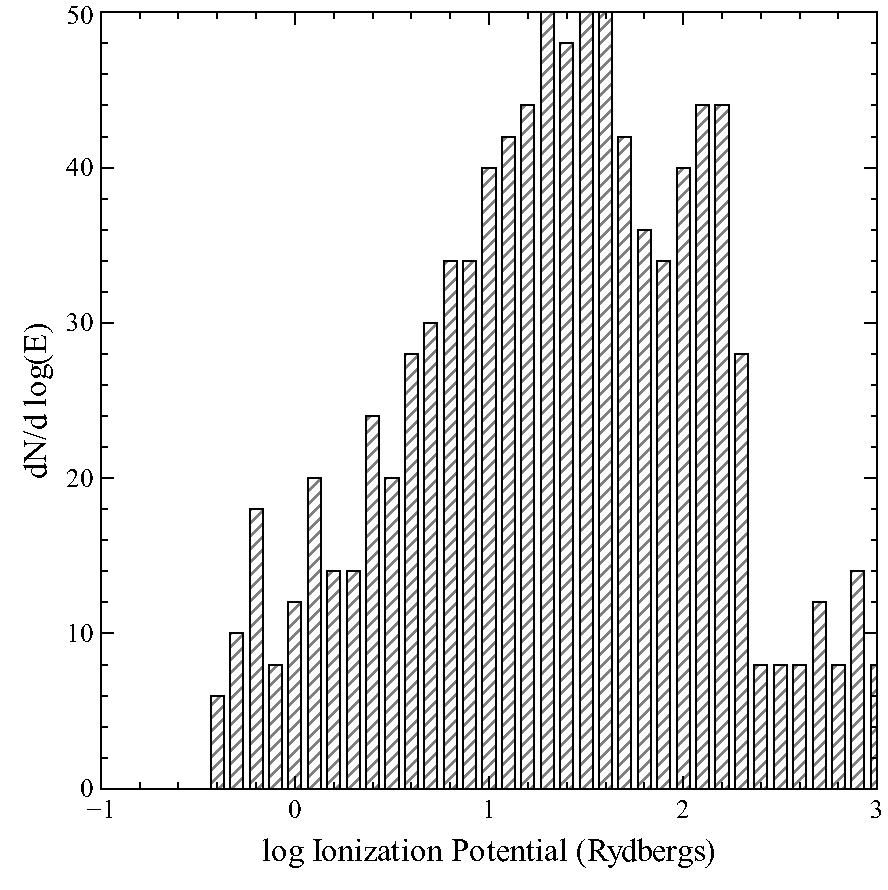
\includegraphics{IonizationPotentials}
\caption[Ionization potentials of the elements]{The number of elements with valence shell ionization potentials
within logarithmically increasing energy widths is shown as a function of
the log off the ionization potential.}
\label{fig:IonizationPotentials}
\end{figure}

\section{Isoelectronic sequences}

Figure \ref{fig:EnergyLevelsSecondRow} shows energy-level diagrams for second row iso-sequences.  For
sequences of elements heavier than K the ground configuration is correct
for ions twice or more times ionized.  For these heavier elements the atom
and first ion may have non-standard configurations for the outer shell.

\begin{figure}
\centering
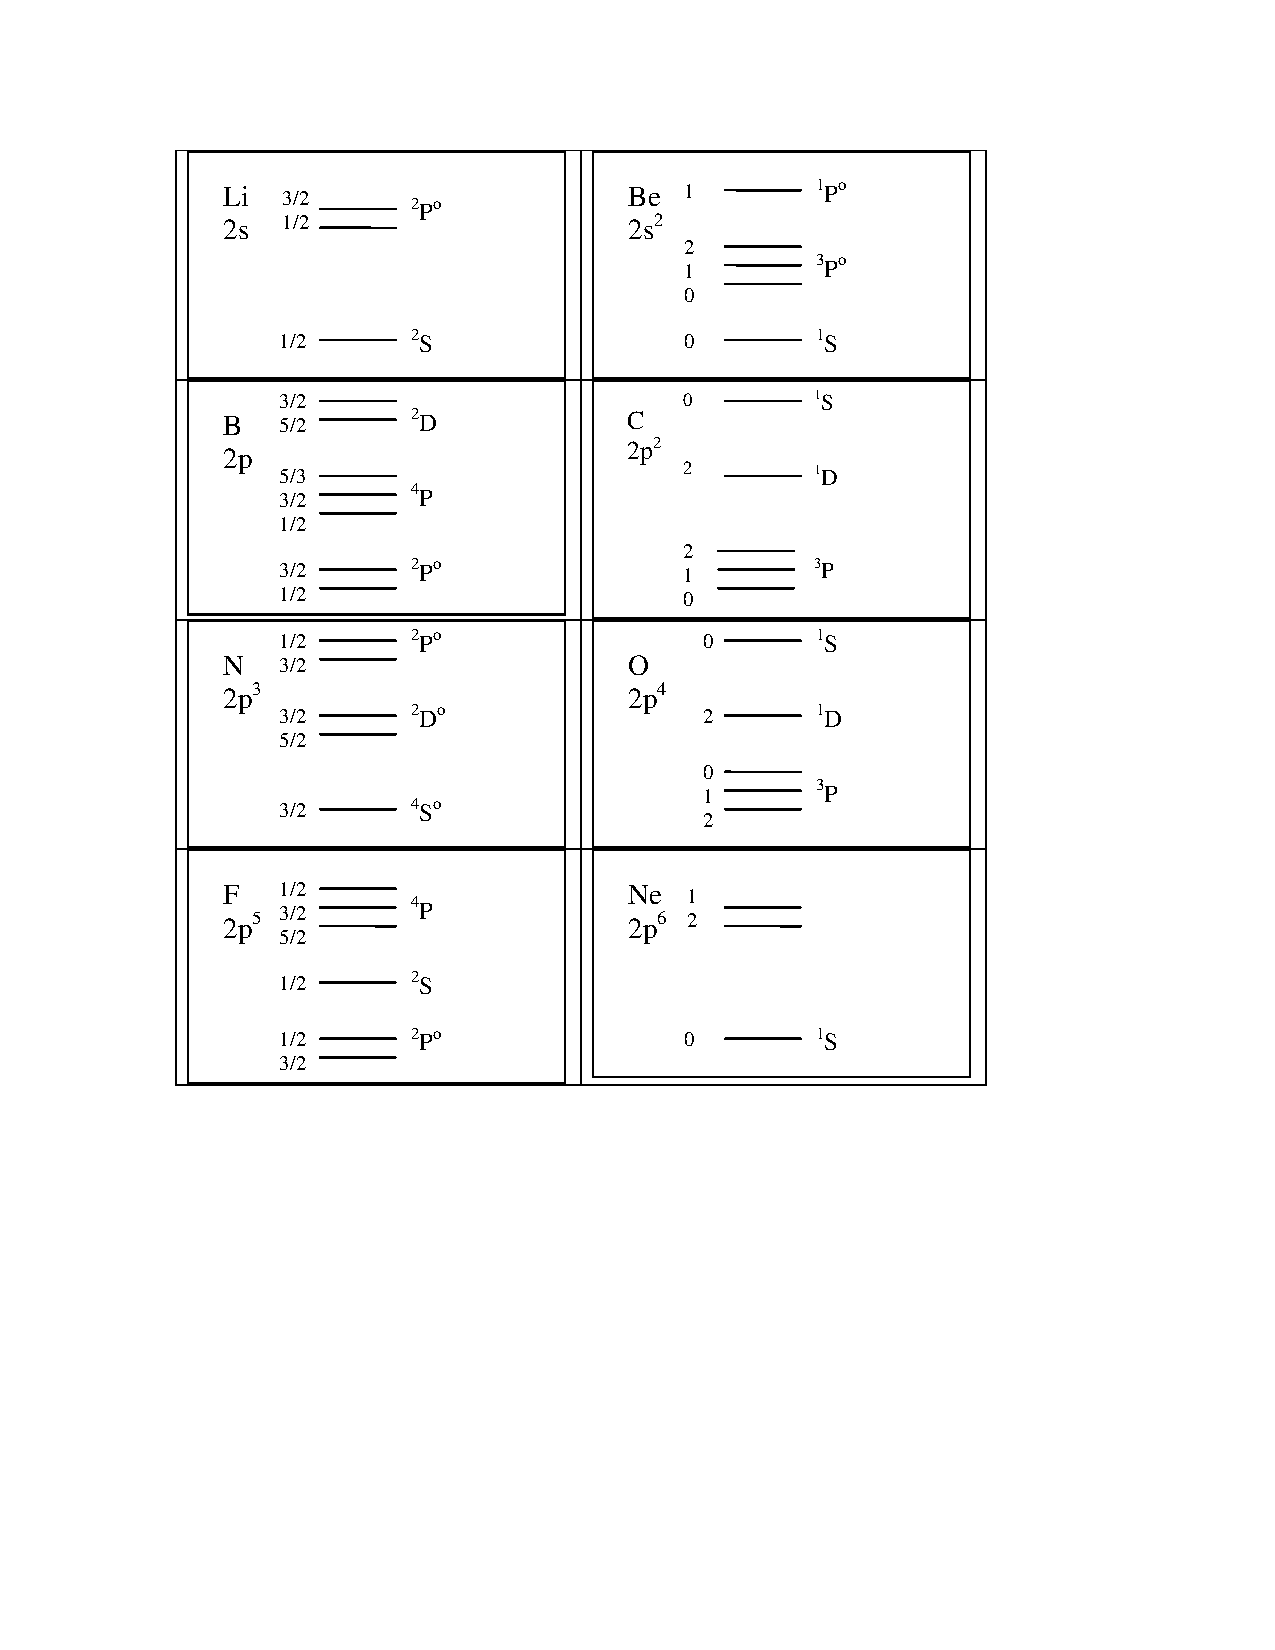
\includegraphics{EnergyLevelsSecondRow}
\caption[Energy level diagrams for second-row elements]{Energy-level diagrams for the second row isoelectronic
sequences. The levels are correct for first ion and higher, but may not
be for some atoms, or for ions of elements with more mass than~K.}
\label{fig:EnergyLevelsSecondRow}
\end{figure}

Table \ref{tab:IsoSequences} lists all isoelectronic sequences for the first thirty elements.
The bottom row on the table indicates the shell number, in the nomenclature
used for the photoionization shell layering\footnote{The arrays within the code count on the C scale so start from 0 and are one less than the index shown in the table.}.
A superscript ``1'' indicates that the atom or first ion has a non-standard configuration in the outer shell.

\begin{table}
\begin{center}
\label{tab:IsoSequences}
\caption{Isoelectronic Sequences}
\begin{tabular}{llllllllll}
\hline
1 H&   2 He&  3 Li&  4 Be&  5 B&  6 C&  7 N&  8 O&  9 F&  10 Ne\\
\hline
1s $^2$S& 1s$^2$ $^1$S& 2s$^2$S& 2s$^2$ $^1$S& 2p $^2$P& 2p$^2$ $^3$P&
2p$^3$ $^4$S& 2p$^4$ $^3$P& 2p$^5$ $^2$P& 2p$^6$ $^1$S\\
H 1& He 1& Li 1& Be 1& Bo 1& C 1& N 1& O 1& F 1& Ne 1\\
He 2& Li 2& Be 2& Bo 2& C 2& N 2& O 2& F 2& Ne 2& Na 2\\
Li 3& Be 3& Bo 3& C 3& N 3& O
3& F 3& Ne 3& Na 3& Mg 3\\
Be 4& Bo 4& C 4& N 4& O 4& F 4& Ne 4& Na 4& Mg 4& Al 4\\
Bo 5& C 5& N 5& O
5& F 5& Ne 5& Na 5& Mg 5& Al 5& Si 5\\
C 6& N 6& O 6& F 6& Ne 6& Na 6& Mg 6& Al 6& Si 6& P 6\\
N 7& O 7& F 7& Ne 7& Na 7& Mg 7& Al 7& Si 7& P 7& S 7\\
O 8& F  8& Ne 8& Na 8& Mg 8& Al 8& Si 8& P  8& S  8&Cl 8\\
F 9& Ne 9& Na 9& Mg 9& Al 9& Si 9& P  9& S 9& Cl 9& Ar 9\\
 Ne10& Na10&Mg10& Al10& Si10& P 10& S
10& Cl10& Ar10& K 10\\
Na11& Mg11& Al11& Si11& P 11& S 11& Cl11& Ar11& K 11& Ca11\\
 Mg12& Al12&
Si12& P 12& S
12& Cl12& Ar12& K 12& Ca12& Sc12\\
Al13& Si13& P 13& S 13& Cl13& Ar13& K 13& Ca13& Sc13& Ti13\\
Si14& P 14&
S 14& Cl14& Ar14& K 14& Ca14& Sc14& Ti14& V 14\\
P 15& S 15& Cl15& Ar15& K 15& Ca15& Sc15& Ti15& V 15& Cr15\\
S 16& Cl16& Ar16& K 16& Ca16& Sc16& Ti16& V 16& Cr16& Mm16\\
Cl17& Ar17&K 17& Ca17& Sc17& Ti17& V 17& Cr17& Mm17& Fe17\\
Ar18& K 18& Ca18& Sc18& Ti18& V 18& Cr18& Mm18& Fe18& Co18\\
K 19& Ca19& Sc19& Ti19& V
19& Cr19& Mm19& Fe19& Co19& Ni19\\
Ca20& Sc20& Ti20& V 20& Cr20& Mm20& Fe20& Co20& Ni20& Cu 20\\
Sc21& Ti21& V
21& Cr21& Mm21& Fe21& Co21& Ni21& Cu 21& Zn 21\\
Ti22& V 22& Cr22& Mm22& Fe22& Co22& Ni22& Cu 22& Zn 22\\
V 23& Cr23& Mm23& Fe23& Co23& Ni23& Cu 23& Zn 23\\
Cr24& Mm24& Fe24& Co24& Ni24& Cu 24& Zn 24\\
Mm25& Fe25& Co25& Ni25& Cu 25& Zn 25\\
Fe26& Co26& Ni26& Cu 26& Zn 26\\
Co27& Ni27& Cu 27& Zn 27\\
Ni28& Cu 28& Zn 28\\
Cu 29& Zn 29\\
Zn 30\\
1&1&2&2&3&3&3&3&3&3\\
\hline
\end{tabular}
\end{center}
\end{table}


\begin{table}
\begin{center}
\addtocounter{table}{-1}
\caption{Isoelectronic Sequences -- Continued}
\begin{tabular}{llllllllll}
\hline
11 Na&  12 Mg&  13 Al&  14 Si&  15 P&   16 S&   17 Cl&  18 Ar&  19 K&   20
Ca\\
\hline
3s $^2$S& 3s$^2$ $^1$S& 3p $^2$P& 3p$^2$ $^3$P& 3p$^3$ $^4$S& 3p$^4$ $^3$P&
3p$^5$ $^2$P& 3p$^6$ $^1$S& 3d $^2$D& 3d$^2$ $^3$F\\
Na 1& Mg 1& Al 1& Si 1& P
1& S  1& Cl 1& Ar 1& K  1$^1$ & Ca 1$^1$\\
Mg 2& Al 2& Si 2& P  2& S  2& Cl 2& Ar 2& K  2& Ca 2$^1$& Sc 2$^1$\\
Al 3& Si
3& P 3& S  3& Cl 3& Ar 3& K  3& Ca 3& Sc 3& Ti 3\\
Si 4& P 4& S  4& Cl 4& Ar 4& K  4& Ca 4& Sc 4& Ti 4& V 4\\
P 5& S  5& Cl 5& Ar 5& K  5& Ca 5& Sc 5& Ti 5& V  5& Cr 5\\
S  6& Cl 6& Ar 6& K  6& Ca 6& Sc 6& Ti 6& V
6& Cr 6& Mm 6\\
Cl 7& Ar 7& K  7& Ca 7& Sc 7& Ti 7& V  7& Cr 7& Mm 7& Fe 7\\
Ar 8& K  8& Ca 8& Sc 8& Ti 8& V
8& Cr 8& Mm 8& Fe 8& Co 8\\
K  9& Ca 9& Sc 9& Ti 9& V  9& Cr 9& Mm 9& Fe 9& Co 9& Ni 9\\
Ca10& Sc10& Ti10& V
10& Cr10& Mm10& Fe10& Co10& Ni10& Cu 10\\
 Sc11& Ti11& V 11& Cr11& Mm11& Fe11& Co11& Ni11& Cu 11& Zn 11\\
 Ti12& V
12& Cr12& Mm12& Fe12& Co12& Ni12& Cu 12& Zn 12\\
V 13& Cr13& Mm13& Fe13& Co13& Ni13& Cu 13& Zn
13\\
Cr14& Mm14& Fe14& Co14& Ni14& Cu 14& Zn 14\\
 Mm15& Fe15& Co15& Ni15& Cu 15& Zn 15\\
Fe16& Co16& Ni16& Cu
16& Zn 16\\
Co17& Ni17& Cu 17&  Zn 17\\
Ni18& Cu 18&  Zn 18\\
Cu 19& Zn 19\\
Zn 20\\
4& 4&5&5&5&5&5&5&6&6\\
\hline
\end{tabular}
\end{center}
\end{table}


\begin{table}
\begin{center}
\addtocounter{table}{-1}
\caption{Isoelectronic Sequences -- Continued}
\begin{tabular}{lllllllllll}
\hline
21 Sc&  22 Ti&  23 V&   24 Cr&  25 Mm&  26 Fe&  27 Co&  28 Ni&  29 Cu& 30
Zn\\
\hline
3d$^3$ $^4$F& 3d$^4$
$^5$D& 3d$^5$ $^6$S& 3d$^6$ $^5$D& 3d$^7$ $^4$F& 3d$^8$ $^3$F& 3d$^9$ $^2$D&
3d$^{10}$ $^1$S& 4s $^2$S& 4s$^2$ $^1$S\\
Sc 1& Ti 1& V  1& Cr 1& Mm 1& Fe
1& Co 1& Ni 1& Cu 1& Zn 1\\
Ti 2& V 2& Cr 2& Mm 2& Fe 2& Co 2& Ni 2& Cu 2& Zn 2\\
V  3& Cr 3& Mm 3& Fe 3& Co
3& Ni 3& Cu 3& Zn 3\\
Cr 4& Mm 4& Fe 4& Co 4& Ni 4& Cu 4& Zn 4\\
Mm 5& Fe 5& Co 5& Ni 5& Cu 5& Zn 5\\
Fe 6& Co
6& Ni 6& Cu 6& Zn 6\\
Co 7& Ni 7& Cu 7& Zn 7\\
Ni 8& Cu 8& Zn 8\\
Cu 9& Zn 9\\
Zn 10\\
6&6&6&6&6&6&6&6&7&7\\
\hline
\end{tabular}
\end{center}
\end{table}

\section{Be-sequence}

The model atom used for Be-like ions (C~III, N~IV, O~V, Al~II, Si~III, S~IV,
etc) is shown in Figure~\ref{fig:BeSequenceEnergyLevels}.

\begin{figure}
\centering
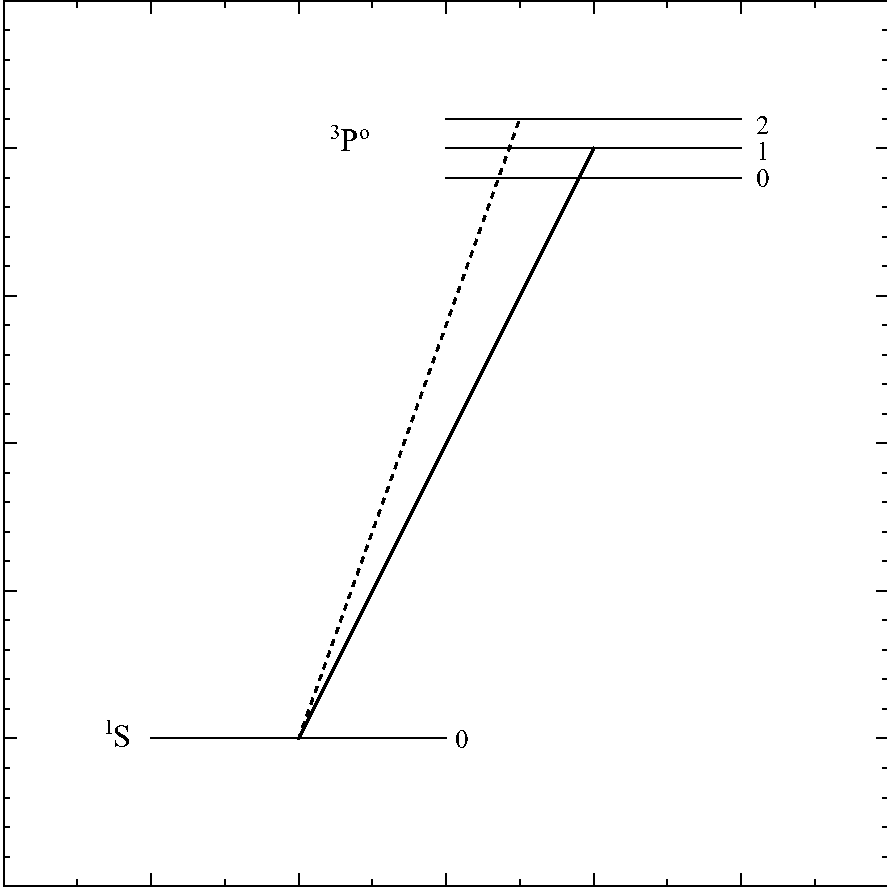
\includegraphics[scale=0.6]{BeSequenceEnergyLevels}
\caption[Be-sequence model atom]{The Be-sequence model atom.  The permitted transition is marked
``UV1,'' while the forbidden and intercombination transitions are ``For''
and ``Int.''}
\label{fig:BeSequenceEnergyLevels}
\end{figure}

\section{Carbon}

\dots

\section{Nitrogen}

Photoionization from the excited $^2D$
level of $N^0$ is included, and can be the dominant ionization mechanism in
well-shielded regions.\footnote{Neutral and first ion have non-standard filling.}

\section{Oxygen}

Photoionization from the first two excited states of O$^{2+}$ is included
as a general ionization mechanism.  This can dominate the ionization of
the ion since it occurs behind the He$^+$ - He$^{++}$ ionization front, which shields
the region from 4 Ryd and higher radiation.   Similarly, photoionization
from the first excited state and all inner shells of $O^0$ are included.

\subsection{The O I model atom}

A partial Grotrian diagram for the O I atom considered in the L$\beta$-O I
fluorescence problem is shown in Figure \ref{fig:OI_EnergyLevels}.  Multiplet averaged transition
probabilities are taken from unpublished Opacity Project data, and the
collision strengths are from the $\bar g$
 approximation for collisions between electrons and neutrals.  Rates
for fluorescence between the two transitions are computed as in
\citet{Netzer1985}.

\begin{figure}
\centering
\includegraphics[scale=0.8]{OI_EnergyLevels}
\caption[O~I energy levels]{The levels of O$^o$ included in the calculation of the
OI-L$_{\beta}$ pumping
problem are shown.}
\label{fig:OI_EnergyLevels}
\end{figure}

\section{Neon}


\section{Magnesium}

Photoionization from the excited $^2P^0$ level of $Mg^+$ is included as a general
$Mg^+$ destruction mechanism using Opacity Project data retrieved from
\cdTerm{TOPBase}.
This can easily be the dominant Mg$^+$ destruction mechanism in
dense gas
since the excited state has an ionization potential below 1 Ryd.  The code
will generate a comment at the end of the calculation if this is a
competitive $Mg^+$ destruction mechanism.

\section{Aluminum}


\section{Calcium}

The Ca II ion is treated as a five-level atom plus continuum.  The model
atom is shown in Figure \ref{fig:CaIIEnergyLevels}, and is similar to that described by \citet{Shine1974}.  Collision strengths for j-mixing collisions are from \citet{Saraph1970}.  Collision and radiative data for the $4s - 4p$ transition are taken
from the compendium of \citet{Mendoza1983}, and all other collision data are
from \citet{Chidichimo1981} and \citet{Saraph1970}.  Radiative data for the $3d - 4p$
and $4s - 3d$ transitions are from
\citet{BlackWeisheit1972}; these
are in good agreement with the calculations of \citet{Osterbrock1951}.  The
compendium by \citet{Shine1974} provides photoionization cross sections
for excited levels, which are adopted here.  Photoionization of the excited
$^2D$ level by \la\ (\citealp{Wyse1941}) and all other line or continuum sources is
explicitly included.  Recombination contributions to the population of
individual levels are included by dividing the excited state recombination
coefficient among the excited levels considered, according to their
statistical weight and the rules of LS coupling.

\begin{figure}
\centering
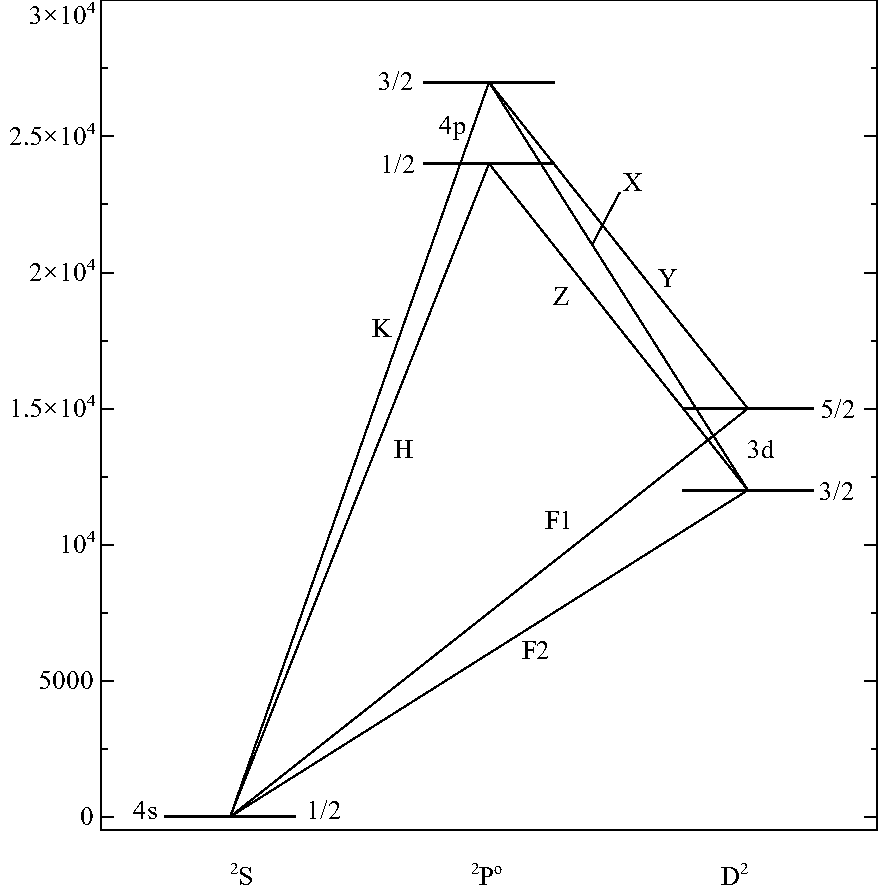
\includegraphics[scale=0.7]{CaIIEnergyLevels}
\caption[CaII model atom]{The five levels of Ca$^+$ included in the calculations are shown.
The wavelengths of the predicted lines are K (3934), H (3969), X (8498),
Y (8542), Z (8662), F1 (7291), and F2 (7324).}
\label{fig:CaIIEnergyLevels}
\end{figure}

All Ca~II transitions (including the forbidden lines) can become quite
optically thick.  Radiative transfer is treated with the escape probability
formalism, assuming incomplete redistribution, including destruction by
background opacities.

\section{Iron}

Low temperature dielectronic recombination rate coefficients have not
been computed for this element.  Means of first-ion rtes are used.  Charge transfer
rate coefficients are from \citet{Neufeld1989} and
\citet{Ferland1997}.

The \feii\ ion is described by \citet{Verner1999} and in sections of
Part I of this document.  In the current implementation up to 376 levels
can be included. This is an area of extensive activity.
Figure \ref{fig:FeII_model} shows
the lowest 16 levels of the atom and some of the lines predicted.

\begin{figure}
\centering
\label{fig:FeII_model}
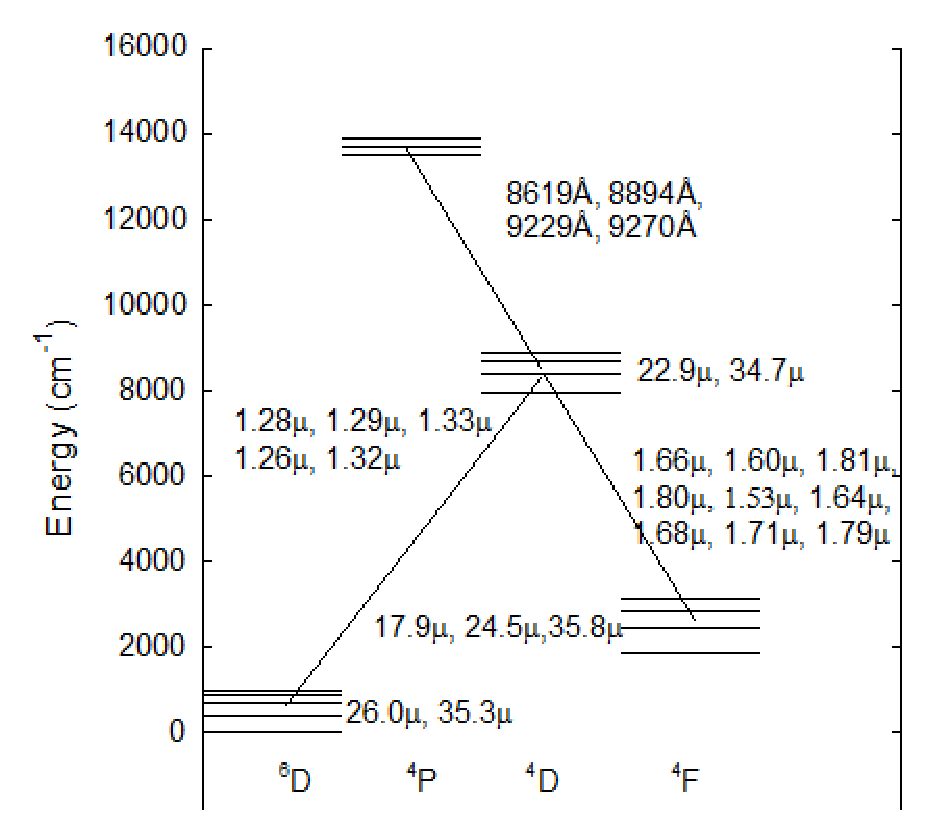
\includegraphics[scale=0.7]{FeII_model}
\caption[\feii\ model of low-lying levels]{The sixteen level atom used to compute \feii\ IR emission.  Lines
predicted are indicated.}
\end{figure}

Fe~IV is treated as a twelve-level atom, with energies from
\citet{Sugar1985}, transition probabilities from \citet{Garstang1958}, and collision
strengths from \citet{Berrington1995}.
Figure \ref{fig:FeIV_model} shows the model atoms
with the lines predicted by the code indicated.

\begin{figure}
\centering
\label{fig:FeIV_model}
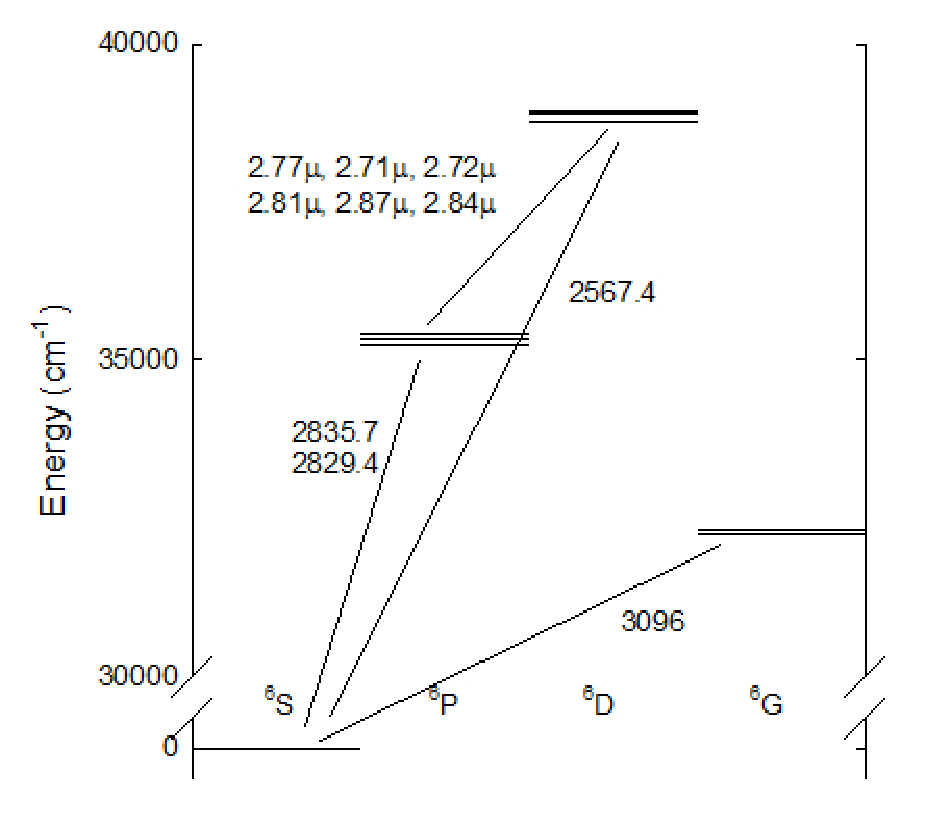
\includegraphics[scale=0.8]{FeIV_model}
\caption[Fe~IV model atom]{The twelve level atom used to compute Fe~IV emission.  Lines
predicted are indicated.}
\end{figure}

Fe~VII is treated as an eight-level system.
Figure \ref{fig:Fe7_levels} shows the levels
and stronger emission lines.
Atomic data are from \citet{Berrington2000}.

\begin{figure}
\centering
\label{fig:Fe7_levels}
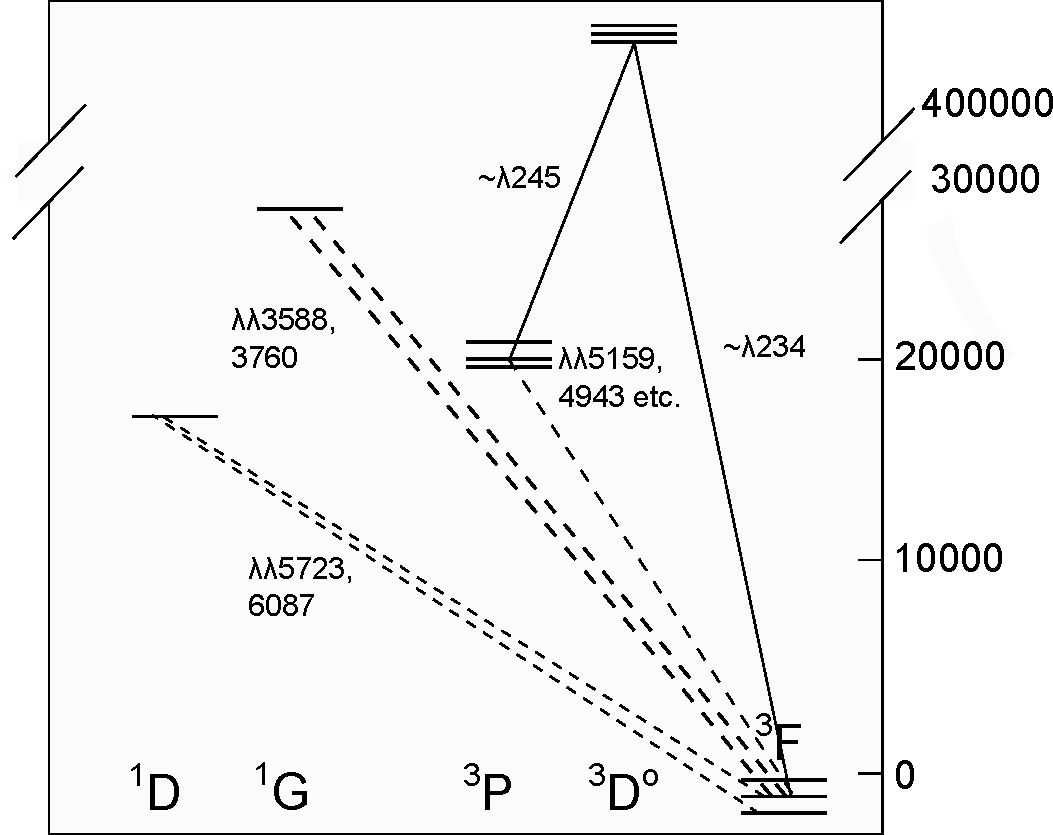
\includegraphics[scale=0.9]{Fe7_levels}
\caption[Fe~VII model atom]{The eight-level atom used to compute Fe~VII emission.  Lines
predicted are indicated.}
\end{figure}

\subsection{Fe K$\alpha$ emission}

The intensity of the Fe~K$\alpha$ line is predicted including both recombination
and fluorescence.  Figure \ref{fig:FeKalpha} shows the fluorescence yield and
K$\alpha$ energy.
The line predictions are separated into ``cold'' iron (i.e., iron with
M-shell electrons present) and ``hot'' iron (those ionization states
producing lines with energies greater than $\sim$6.4 keV).  This includes the
recombination and collisional contribution.  The ``TOTL'' K$\alpha$ is the sum of
the two.

\begin{figure}
\centering
\label{fig:FeKalpha}
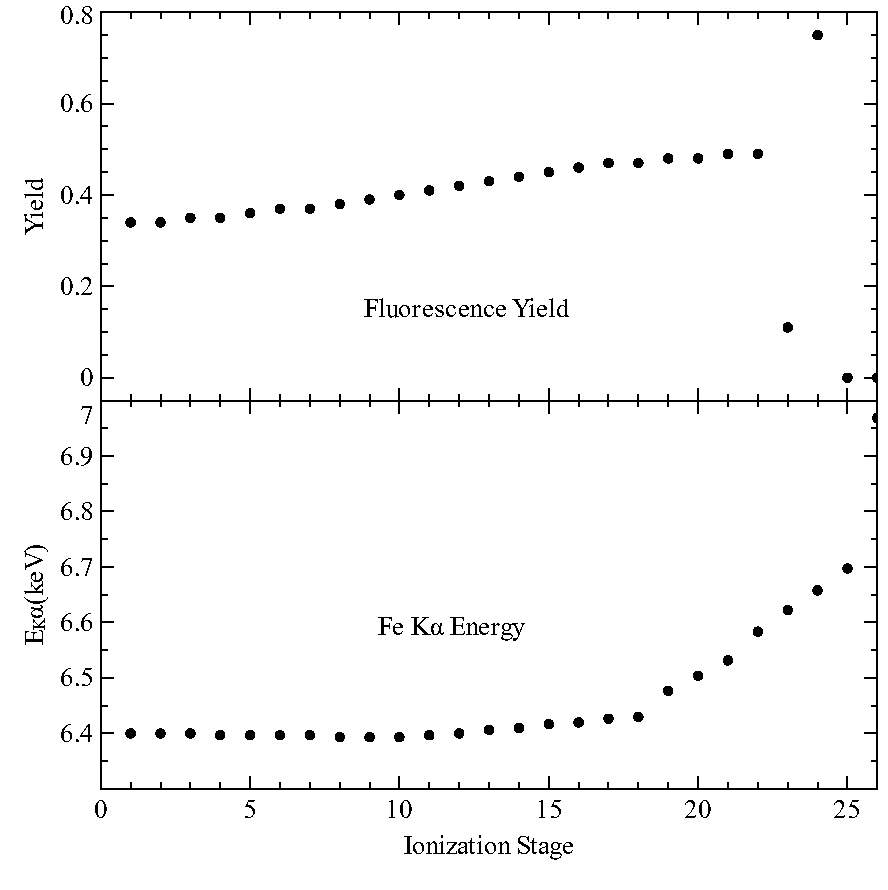
\includegraphics[scale=0.8]{FeKalpha}
\caption[Fe~K$\alpha$ yield and energy]{The fluorescence yield and energy of the emitted Fe~K$\alpha$ photon
are shown as a function of ionization stage.}
\end{figure}

\section{Heavy element opacities}

Figure \ref{fig:GasOpacity} shows a calculation of the opacity of a solar gas with very
low ionization.

\begin{figure}
\centering
\label{fig:GasOpacity}
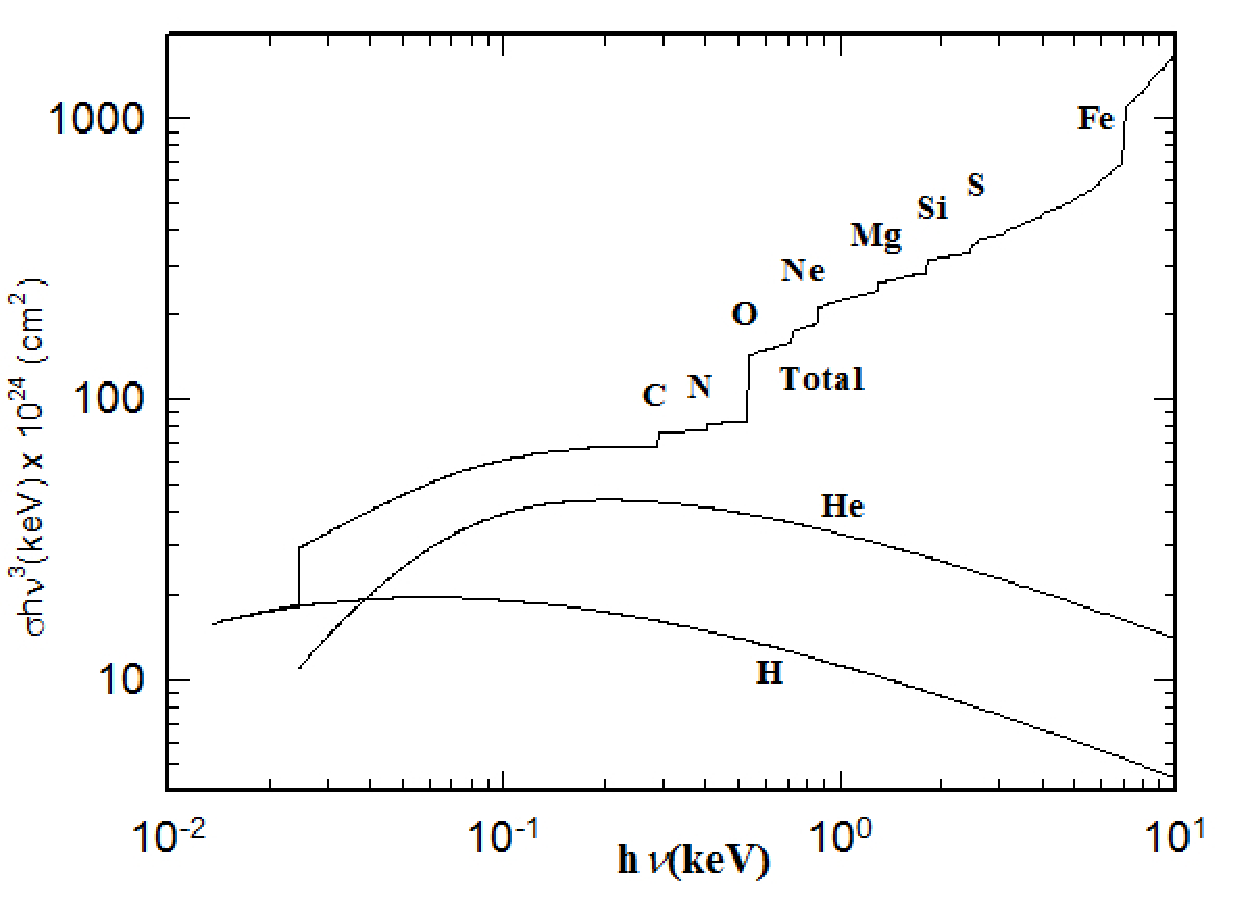
\includegraphics[scale=0.7]{GasOpacity}
\caption[Atomic gas opacity]{The opacity of a neutral gas with solar abundances is shown
as a function of energy.  The curve is scaled to allow direct comparison
with conventional calculations of opacity at X-Ray energies (i.e., \citet{Morrison1983}. hevopc}
\end{figure}

\section{Overall reliability}

It is difficult to estimate the overall uncertainty present in an
ionization balance calculation.  The current photoionization cross-section
data are based on accurate experiments or the Opacity Project (\citealp{VernerFerlandKorista1996}).  These should be accurate to roughly 10\% except near resonances.
Although resonances are included in the Opacity Project data, the positions
of these resonances are uncertain by more than their width because the OP
was not intended as an atomic structure calculation.  Recombination
coefficients including low temperature dielectronic recombination have yet
to be computed for the majority of the stages of ionization of the elements
now in \Cloudy, but recombination from parent ions with closed shells is
not affected, and good rates exist \citep{VernerFerland1996}.

It is possible to make a subjective estimate of the uncertainty in the
calculation of the ionization balance for nebular temperatures.
Table~\ref{tab:IonizationBalanceReliability}
lists the elements now included in the calculations and gives this estimate
of the uncertainty.  For recombination from a closed shell autoionization
resonances do not occur near threshold, recombination is primarily radiative,
and the calculations should be virtually exact.  Dielectronic recombination
rates are also known for those species treated by
Nussbaumer and Storey.
These are given a quality weighting of~A.

\begin{table}
\begin{center}
\caption{Ionization Balance Reliability}
\label{tab:IonizationBalanceReliability}
\begin{tabular}{lllllllllll}
\hline
1& H&2 He&3 Li&4 Be&5 B&6 C&7 N&8 O&9 F&10 Ne\\
\hline
1&A&A&A&B&B&B&B&B&B&B\\
2&& A&A&A&B&B&B&B&B&B\\
3&&&A&A&A&B&B&B&B&B\\
4&&&&A&A&A&B&B&B&B\\
5&&&&&A&A&A&B&B&B\\
6&&&&&&A&A&A&B&B\\
7&&&&&&&A&A&A&B\\
8&&&&&&&&A&A&A\\
9&&&&&&&&&A&A\\
10&&&&&&&&&&A\\
\hline
\end{tabular}
\end{center}
\end{table}


\begin{table}
\addtocounter{table}{-1}
\begin{center}
\caption{Ionization Balance Reliability -- Continued}
\begin{tabular}{lllllllllllll}
\hline
&11 Na&12 Mg&13 Al&14 Si&15 P&16 S&17 Cl&18 Ar&19 K&20 Ca\\
\hline
1&B&B\\
2&B&B&B\\
3&B&B&B&B\\
4&B&B&B&B&B\\
5&B&B&B&B&B&B\\
6&B&B&B&B&B&B&B\\
7&B&B&B&B&B&B&B&B\\
8&B&B&B&B&B&B&B&B&B\\
9&A&B&B&B&B&B&B&B&b&B\\
10&A&A&B&B&B&B&B&B&B&B\\
11&A&A&A&B&B&B&B&B&B&B\\
12&&A&A&A&B&B&B&B&B&B\\
13&&&A&A&A&B&B&B&B&B\\
14&&&&A&A&A&B&B&B&B\\
15&&&&&A&A&A&B&B&B\\
16&&&&&&A&A&A&B&B\\
17&&&&&&&A&A&A&B\\
18&&&&&&&&A&A&A\\
19&&&&&&&&&A&A\\
20&&&&&&&&&&A\\
\hline
\end{tabular}
\end{center}
\end{table}


\begin{table}
\addtocounter{table}{-1}
\begin{center}
\caption{Ionization Balance Reliability -- Continued}
\begin{tabular}{lllllllllllll}
\hline
&21 Sc&22 Ti&23 V&24 Cr&25 Mn&26 Fe&27 Co&28 Ni&29 Cu&30
Zn&\\
1\\
2\\
3\\
4\\
5\\
6\\
7\\
8\\
9\\
10&B\\
11&B&B\\
12&B&B&B&\\
13&B&B&B&B\\
14&B&B&B&B&B\\
15&B&B&B&B&B&B\\
16&B&B&B&B&B&B&B\\
17&B&B&B&B&B&B&B&B\\
18&B&B&B&B&B&B&B&B&B\\
19&A&B&B&B&B&B&B&B&B&B\\
20&A&A&B&B&B&B&B&B&B&B\\
21&A&A&A&B&B&B&B&B&B&B\\
22&&A&A&A&A&B&B&B&B&B\\
23&&&A&A&A&B&B&B&B&B\\
24&&&&A&A&A&B&B&B&B\\
25&&&&&A&A&A&B&B&B\\
26&&&&&&A&A&A&B&B\\
27&&&&&&&A&A&A&B\\
28&&&&&&&&A&A&A\\
29&&&&&&&&&A&A\\
30&&&&&&&&&&A\\
\hline
\end{tabular}
\end{center}
\end{table}

These uncertainties refer to the ionization balance of an optically thin
cell of gas at nebular temperatures.  The intensities of emission lines
will be less uncertain than this for two reasons. First, the thermostat
effect of any collisionally excited line prevents its intensity from changing
by much.  Second is the fact that the integrated column density in an ion
is affected as much by (fairly exact) quantities such as the ionization
structure of H or He, as by the atomic data of a particular ion.  At coronal
temperatures the Burgess mechanism dominates, and the situation should be
somewhat better.

Nigel Badnell and collaborators have begun a program to compute
dielectronic recombination rate coefficients along isoelectronic sequences.
These have appeared in a series of papers in A\&A starting in 2003.  Ions
which have been done by Badnell et al. appear as B in the table.  They have
not yet produced radiative recombination rates.

\section{Solving the ionization ladder }

   The rate of change of the density of a particular ionization state i
is given by
\begin{equation}
\frac{{\partial {n_i}}}{{\partial t}} = {G_i} + \sum\limits_{j \ne i}
{{R_{j \to i}}{n_j}}  - {n_i}\left( {{L_i} + \sum\limits_{j \ne i} {{R_{i
\to j}}} } \right)\quad
[\mathrm{cm}^{-3} \mathrm{s}^{-1}].% (1)
\end{equation}
Gains $G_i$ [cm$^{-3}$~s$^{-1}$] and losses $L_i$~[s$^{-1}$] represent physical processes that
remove atoms from the ionization ladder.  Advection, or molecular processes
that create or destroy atoms and ions, are examples.  The terms $R_{nm}$ are
rates (s$^{-1}$) for processes that move atoms up or down the ionization ladder.

Several physical processes strongly couple
non-adjacent stages of ionization.  Charge transfer on grain surfaces and
advection are examples.  The full system of equations is solved using standard
linear algebra methods.

\section{Ionization potentials of subshells}

Table \ref{tab:SubshellIonizationPotentials} gives ionization potentials
of the subshells.

\begin{table}
\begin{center}
\label{tab:SubshellIonizationPotentials}
\caption{Ionization Potentials of Subshells (eV)}
\begin{tabular}{lllllllllll}
\hline
Element\\
\hline
H&    1\\
\hline
1s& 13.60\\
\hline
He&   1&   2\\
\hline
1s& 24.59& 54.42\\
\hline
Li&   1&   2&   3\\
\hline
1s& 64.39& 75.64& 122.5\\
2s& 5.392\\
\hline
Be&   1&   2&   3&   4\\
\hline
1s& 119.3& 129.9& 153.9& 217.7\\
2s& 9.323& 18.21\\
\hline
B& 1&   2&   3&   4&   5\\
\hline
1s& 194.0& 209.8& 227.4& 259.4& 340.2\\
2s& 14.05& 25.16& 37.93\\
2p& 8.298\\
\hline
C&    1&   2&   3&   4&   5&   6\\
\hline
1s& 291.0& 307.6& 328.9& 352.2& 392.1& 490.0\\
2s& 19.39& 30.47& 47.89& 64.49\\
2p& 11.26& 24.38\\
\hline
N&    1&   2&   3&   4&   5&   67   7\\
\hline
1s& 404.8&
423.6& 447.3& 475.3& 504.3& 552.1& 667.1\\
2s& 25.41& 37.96& 55.45& 77.47& 97.89\\
2p& 14.53&
29.60& 47.45\\
\hline
O& 1& 2& 3& 4& 5& 6& 7& 8\\
\hline
1s& 538.0& 558.1& 584.0& 614.4&
649.1& 683.7& 739.3& 871.4\\
2s& 28.48& 45.99& 65.51& 87.37& 113.9& 138.1\\
2p& 13.62& 35.12&
54.94& 77.41\\
\hline
F&    1&   2&   3&   4&   5&   6&   7&   8&   9\\
\hline
1s& 694.0& 712.2& 739.2& 770.9&
809.1& 850.2& 890.5& 953.9&  1103\\
2s& 37.86& 54.59& 76.10& 99.57& 126.2& 157.2& 185.2\\
2p& 17.42& 34.97& 62.71& 87.14& 114.2\\
\hline
\end{tabular}
\end{center}
\end{table}


\begin{table}
\begin{center}
\addtocounter{table}{-1}
\caption{Ionization Potentials of Subshells (eV) -- Continued}
\begin{tabular}{lllllllllll}
\hline
Ne&   1&   2&   3&   4&   5&   6&   7&   8&   9&  10\\
\hline
1s& 870.1& 883.1& 913.1& 948.0& 987.3&
1031&  1078&  1125&  1196&  1362\\
2s& 48.47& 63.74& 87.21& 113.2& 141.5& 171.9& 207.3&
239.1\\
2p& 21.56& 40.96& 63.46& 97.12& 126.2& 157.9\\
\hline
Na&   1&   2&   3&   4&   5&   6& 7&   8&   9&  10\\
\hline
1s&  1079&  1097&  1118&  1143&  1185&  1230&  1281&  1335&  1386&  1465\\
2s&
70.84& 73.47& 99.45& 126.9& 156.7& 189.9& 224.4& 264.2& 299.9\\
2p& 38.14& 47.29& 71.62&
98.92& 138.4& 172.2& 208.5\\
3s& 5.139\\
\hline
Na&  11\\
\hline
1s&  1649\\
\hline
Mg&   1&   2&   3&   4&   5&   6& 7&   8&   9&  10\\
\hline
1s&  1311&  1320&  1336&  1356&  1400&  1449&  1501&  1558&  1618&  1675\\
2s&
94.00& 98.81& 111.1& 141.1& 173.5& 207.6& 244.4& 283.9& 328.2& 367.5\\
2p& 54.90& 65.69&
80.14& 109.3& 141.3& 186.5& 224.9& 266.0\\
3s& 7.646& 15.04\\
\hline
Mg&  11&  12\\
\hline
1s&  1762&  1963\\
\hline
Al& 1&   2&   3&   4&   5&   6&   7&   8&   9&  10\\
\hline
1s&  1567&  1571&  1583&  1604&  1634&  1688&
1739&  1799&  1862&  1929\\
2s& 125.6& 128.1& 140.7& 155.8& 190.3& 226.8& 266.2& 306.5&
350.2& 399.4\\
2p& 80.40& 89.97& 102.6& 120.0& 153.8& 190.5& 241.4& 284.6& 330.1\\
3s& 11.33&
18.83& 28.45\\
3p& 5.986\\
\hline
Al&  11&  12&  13\\
\hline
1s&  1992&  2086&  2304\\
2s& 442.1\\
\hline
Si& 1&   2&
3&   4&   5&   6&   7&   8&   9&  10\\
\hline
1s&  1846&  1848&  1852&  1868&  1887&  1946&  2001&
2058&  2125&  2194\\
2s& 156.0& 161.9& 174.4& 189.9& 207.6& 246.8& 287.2& 331.0& 375.6&
423.4\\
2p& 106.0& 118.6& 131.1& 146.6& 166.8& 205.1& 246.5& 303.2& 351.1& 401.4\\
3s& 15.17&
22.40& 33.49& 45.143p& 8.152& 16.35\\
\hline
\end{tabular}
\end{center}
\end{table}


\begin{table}
\begin{center}
\addtocounter{table}{-1}
\caption{Ionization Potentials of Subshells (eV) -- Continued}
\begin{tabular}{llllllllllll}
\hline
Si&  11&  12&  13&  14\\
\hline
1s&  2268&  2336&  2438&  2673\\
2s& 476.1& 523.5\\
P&    1&   2&   3&
4&   5&   6&   7&   8&   9&  10\\
1s&  2154&  2155&  2157&  2173&  2192&  2214&  2280&  2337&
2407&  2477\\
2s& 194.0& 198.7& 212.4& 228.0& 246.1& 266.3& 309.8& 355.2& 401.8& 452.2\\
2p&
140.0& 149.5& 163.9& 179.5& 197.7& 220.4& 263.2& 309.4& 371.7& 424.5\\
3s& 20.17& 27.09&
38.28& 51.44& 65.03\\3p& 10.49& 19.73& 30.20\\
\hline
P&   11&  12&  13&  14&  15\\
\hline
1s&  2553&  2633&
2707&  2817&  3070\\
2s& 503.5& 560.4& 611.9\\
2p& 479.6\\
\hline
S&    1&   2&   3&   4&   5&   6&
7&  8&   9&  10\\
\hline
1s&  2477&  2478&  2486&  2502&  2522&  2544&  2569&  2641&  2705&  2782\\
2s&
235.0& 238.7& 253.6& 270.3& 288.8& 309.4& 332.1& 379.7& 429.6& 480.4\\
2p& 170.0& 184.6&
199.5& 216.4& 235.0& 255.7& 280.9& 328.2& 379.1& 447.1\\
3s& 21.30& 31.90& 44.15& 57.50&
72.68& 88.05\\
3p& 10.36& 23.33& 34.83& 47.31\\
\hline
S&   11&  12& 13&  14&  15&  16\\
\hline
1s&  2859&
2941&  3029&  3107&  3224&  3494\\
2s& 534.6& 590.6& 651.7& 707.2\\
2p& 504.8& 564.7\\
\hline
Cl&
1&   2&   3&   4&   5&   6&   7&   8&   9&  10\\
\hline
1s&  2830&  2832&  2838&  2851&  2875&  2898&
2923&  2951&  3030&  3100\\
2s& 278.0& 283.7& 297.9& 315.1& 335.4& 356.6& 379.7& 404.8&
456.5& 510.9\\
2p& 209.0& 223.6& 238.2& 255.2& 276.0& 297.4& 320.7& 348.3& 400.1& 455.6\\
3s&
25.31& 36.86& 50.19& 64.70& 79.97& 97.03& 114.2\\
3p& 12.97& 23.81& 39.61& 53.47& 67.82\\
\hline
Cl&
11&  12&  13&  14&  15&  16&  17\\
\hline
1s&  3184&  3266&  3356&  3448&  3534&  3659&  3946\\
2s&
566.0& 624.9& 684.6& 749.8& 809.4\\
2p& 529.3& 592.0& 656.7\\
\hline
\end{tabular}
\end{center}
\end{table}


\begin{table}
\begin{center}
\addtocounter{table}{-1}
\caption{Ionization Potentials of Subshells (eV) -- Continued}
\begin{tabular}{lllllllllll}
\hline
Ar&   1&   2&   3&   4&   5&   6&   7&   8&   9&  10\\
\hline
1s& 3203&  3208&  3216&  3228&  3253&
3277&  3303&  3331&  3361&  3446\\
2s& 326.0& 331.7& 345.5& 364.2& 385.2& 407.6& 431.4&
457.0& 484.5& 540.3\\
2p& 249.2& 266.2& 280.1& 298.7& 320.0& 342.6& 366.7& 392.5& 422.5&
478.7\\
3s& 28.92& 41.98& 56.37& 71.74& 88.28& 105.6& 124.3& 143.5\\
3p& 15.76& 27.63& 40.74&
59.81& 75.02& 91.01\\
\hline
Ar&  11&  12&  13&  14&  15&  16&  17& 18\\
\hline
1s& 3523& 3613& 3702&
3798&  3898&  3988&  4121&  4426\\
2s& 599.2& 658.4& 721.7& 785.6& 854.8& 918.0\\
2p& 539.0&
618.3& 686.1& 755.8\\
\hline
K&    1&   2&   3&   4&   5&   6&   7&   8&   9&  10\\
\hline
1s&  3614&  3617&
3623&  3633&  3651&  3679&  3706&  3735&  3766& 3799\\
2s& 384.3& 386.7& 399.0& 416.5&
437.4& 461.8& 486.8& 513.3& 541.3& 571.2\\
2p& 301.4& 306.7& 327.9& 345.2& 366.5& 390.9&
416.2& 443.0& 471.3& 503.8\\
3s& 40.80& 47.28& 62.69& 79.25& 96.57& 115.2& 134.4& 154.7&
175.8\\
3p& 24.66& 31.63& 45.81& 60.91& 82.66& 99.44& 117.6\\
3d& 1.000\\
4s& 4.341\\
\hline
K&   11
12&  13&  14&  15&  16&  17&  18&  19\\
\hline
1s&  3890&  3974&  4070&  4166&  4269&  4375&  4471&
4611&  4934\\
2s& 631.0& 694.5& 757.8& 825.5& 893.5& 968.0&  1035\\
2p& 564.7& 629.5& 714.7&
786.7& 861.1\\
\hline
Ca&   1&   2&   3&   4&   5&   6&   7&   8&   9&  10\\
\hline
1s&  4043&  4047&  4053&
4063&  4078&  4105&  4133&  4163&  4198&  4229\\
2s& 442.5& 444.5& 454.2& 471.9& 494.8&
519.3& 545.5& 573.2& 601.8& 632.6\\
2p& 352.3& 363.8& 373.1& 394.4& 417.5& 442.3& 468.7&
496.7& 527.0& 556.9\\
3s& 48.30& 60.37& 69.20& 86.80& 105.4& 124.9& 145.2& 166.4& 188.3&
211.3\\
3p& 34.43& 40.90& 50.91& 67.27& 84.51& 108.8& 127.2& 147.2\\
3d& 1.000& 1.000\\
4s&
6.113& 11.87\\
\hline
Ca&  11&  12&  13&  14&  15&  16&  17&  18&  19&  20\\
\hline
1s&  4265&  4362&  4453&
4555&  4659&  4767&  4880&  4982&  5129&  5470\\
2s& 664.9& 728.7& 796.8& 864.2& 935.7&
1008& 1087& 1157\\
2p& 591.9& 657.2& 726.7& 817.7& 894.6& 974.5\\
\hline
\end{tabular}
\end{center}
\end{table}


\begin{table}
\begin{center}
\addtocounter{table}{-1}
\caption{Ionization Potentials of Subshells (eV) -- Continued}
\begin{tabular}{lllllllllll}
\hline
Sc&   1&   2&   3&   4&   5&   6&   7&   8&   9&  10\\
\hline
1s&  4494&  4500&  4508&  4517&  4531&
4554&  4582&  4615&  4649&  4684\\
2s& 503.2& 505.4& 514.8& 530.6& 555.2& 580.3& 605.2&
636.2& 666.6& 698.2\\
2p& 405.4& 419.0& 428.5& 447.6& 473.0& 497.7& 523.6& 554.4& 585.2&
617.3\\
3s& 56.40& 68.48& 77.62& 94.51& 114.1& 134.8& 155.7& 178.4& 201.5& 225.1\\
3p& 33.60&
46.78& 55.91& 73.49& 91.87& 110.7& 138.0& 158.1& 180.0\\
3d& 8.010& 14.44& 24.76\\
4s& 7.342&
12.80\\
\hline
Sc& 11& 12&  13&  14&  15&  16&  17&  18&  19&  20\\
\hline
1s&  4720&  4759&  4861&  4960&
5067&  5178&  5294&  5413&  5520&  5675\\
2s& 730.9& 765.7& 833.3& 906.2& 977.5& 1054&
1130& 1213& 1288\\
2p& 650.5& 687.4& 756.7& 830.8& 927.5&  1009&  1094\\
3s& 249.8\\
\hline
Sc&
21\\
\hline
1s&  6034\\
\hline
Ti&   1&   2&   3&   4&   5&   6&   7&   8&   9&  10\\
\hline
1s&  4972&  4980&  4988&
4998&  5011&  5027&  5059&  5089&  5126&  5162\\
2s& 569.0& 570.4& 579.2& 594.9& 617.8&
644.1& 672.9& 699.9& 734.2& 767.0\\
2p& 464.0& 477.2& 487.0& 506.6& 529.6& 556.3& 585.3&
612.9& 647.3& 680.7\\
3s& 65.00& 76.54& 86.03& 103.5& 123.1& 144.5& 167.3& 190.0& 214.8&
239.7\\
3p& 40.00& 52.53& 62.01& 79.17& 99.30& 119.5& 140.8& 170.4& 192.1& 215.9\\
3d&
9.940&
16.13& 27.49& 43.27\\
4s& 6.820& 13.58\\
\hline
Ti&  11&  12&  13&  14&  15&  16&  17&  18&  19&  20\\
\hline
1s&
5200&  5239&  5281&  5387&  5495&  5607&  5726&  5848&  5974&  6087\\
2s& 801.3& 836.3&
873.4& 944.8& 1022& 1098& 1179& 1260& 1346& 1425\\
2p& 715.6& 751.1& 787.8& 863.1&
941.9&  1044&  1131&  1221\\
3s& 265.0& 291.5\\
\hline
Ti& 21&  22\\
\hline
1s&  6249&  6626\\
\hline
V&  1&   2& 3&   4&   5&   6&   7&   8&   9&  10\\
\hline
1s&  5475&  5484&  5493&  5504&  5516&  5531&  5557&
5591&  5624&  5664\\
2s& 638.0& 638.9& 642.1& 665.4& 685.9& 712.3& 740.1& 772.7& 801.7&
839.1\\
2p& 527.0& 529.2& 548.7& 571.5& 592.3& 618.8& 646.8& 680.0& 709.3& 747.4\\
3s& 77.00&
79.42& 94.52& 111.8& 132.9& 154.9& 178.1& 203.1& 227.4& 254.3\\
3p& 47.00& 53.23& 68.13&
85.55& 105.9& 128.1& 150.6& 173.5& 205.8& 230.5\\
3d& 12.00& 14.66& 29.31& 46.71& 65.28\\
4s&
6.740\\
\hline
\end{tabular}
\end{center}
\end{table}


\begin{table}
\begin{center}
\addtocounter{table}{-1}
\caption{Ionization Potentials of Subshells (eV) -- Continued}
\begin{tabular}{lllllllllll}
\hline
V&   11&  12& 13&  14&  15&  16&  17&  18&  19&  20\\
\hline
1s&  5704&  5745&  5787&  5831&  5941&
6058&  6174&  6302&  6431&  6563\\
2s& 874.6& 911.4& 948.8& 988.3& 1063& 1146& 1225&
1311&  1396&  1487\\
2p& 783.4& 820.9& 858.9& 896.0& 975.8&  1060&  1168&  1260&  1355\\
3s&
281.0& 308.1& 336.3\\
3p& 255.7\\
\hline
V&   21&  22&  23\\
\hline
1s&  6682&  6852&  7246\\
2s&  1570\\
\hline
Cr& 1&   2&   3&   4&   5&   6&   7&   8&   9&  10\\
\hline
1s&  5996&  6009&  6021&  6033&  6046&  6062&
6080&  6114&  6152&  6187\\
2s& 703.0& 707.4& 716.1& 733.1& 759.8& 784.2& 814.0& 843.2&
879.7& 910.8\\
2p& 585.0& 597.0& 616.4& 634.4& 660.2& 685.5& 715.3& 744.4& 781.9& 813.0\\
3s&
79.00& 87.45& 103.2& 121.9& 142.7& 165.6& 190.0& 214.8& 241.9& 268.0\\
3p& 49.00& 58.79&
74.36& 92.75& 113.4& 135.9& 160.2& 184.7& 209.3& 244.4\\
3d& 8.660& 16.50& 30.96& 49.16&
69.46& 90.64\\
4s& 6.767\\
\hline
Cr&  11&  12&  13&  14&  15&  16&  17&  18&  19&  20\\
\hline
1s&  6231&  6274&
6318&  6362&  6409&  6523&  6650&  6769&  6907&  7042\\
2s& 951.2& 989.3&  1029&  1068&
1110&  1189&  1276&  1359&  1450&  1539\\
2p& 854.6& 893.3& 933.4& 973.8& 1011& 1097&
1185&  1299&  1396&  1497\\
3s& 296.9& 325.5& 354.8& 384.2\\
3p& 270.8& 298.1\\
\hline
Cr&  21&  22& 23&  24\\
\hline
1s&  7181&  7306&  7482&  7895\\
2s&  1634&  1721\\
\hline
Mn&   1&   2&   3&   4&   5&   6&
7&   8&   9&  10\\
\hline
1s&  6550&  6564&  6576&  6589&  6602&  6617&  6635&  6664&  6698&  6741\\
2s&
781.6& 784.9& 794.7& 811.8& 831.9& 861.4& 890.0& 923.0& 953.6& 993.9\\
2p& 655.4& 671.4&
682.2& 706.3& 728.0& 756.0& 786.0& 819.1& 849.2& 891.03\\
s& 94.60& 101.5& 112.0& 130.0&
153.0& 176.8& 201.6& 228.2& 254.7& 284.0\\
3p& 59.40& 70.09& 80.62& 98.79& 121.0& 144.4&
169.1& 194.5& 221.8& 248.3\\
3d& 14.30& 20.58& 33.67& 51.20& 72.40& 95.75& 119.3\\
4s& 7.434&
15.64\\
\hline
\end{tabular}
\end{center}
\end{table}


\begin{table}
\begin{center}
\addtocounter{table}{-1}
\caption{Ionization Potentials of Subshells (eV) -- Continued}
\begin{tabular}{lllllllllll}
\hline
Mn&  11&  12&  13&  14&  15&  16&  17&  18&  19&  20\\
\hline
1s&  6778&  6826&  6872&  6919&  6966&
7016&  7132&  7270&  7391&  7539\\
2s&  1027&  1070&  1111&  1153&  1195&  1239&  1321&
1414&  1500&  1596\\
2p& 923.8& 969.0& 1010&  1053&  1096&  1133&  1224&  1317&  1437&
1539\\
3s& 311.8& 342.7& 373.1& 403.0& 435.2\\
3p& 286.0& 314.4& 343.6\\
\hline
Mn&  21&  22&  23&
24& 25\\
\hline
1s& 7682&  7827&  7957&  8141&  8572\\
2s&  1689&  1788&  1880\\
2p&  1644\\
\hline
Fe& 1& 2&   3&   4&   5&   6&   7&   8&   9&  10\\
\hline
1s&  7124&  7140&  7155&  7169&  7184&  7199&
7217&  7237&  7275&  7316\\
2s& 857.0& 860.8& 871.0& 887.1& 910.1& 938.3& 969.3& 1003&
1039&  1076\\
2p& 724.0& 734.1& 745.1& 766.9& 792.0& 820.2& 851.2& 884.9& 921.1& 959.0\\
3s&
104.0& 110.2& 121.1& 141.1& 163.3& 187.6& 213.5& 240.9& 269.6& 299.0\\
3p& 66.00& 76.17&
87.05& 106.7& 128.8& 152.7& 178.3& 205.5& 233.6& 262.1\\
3d& 14.70& 21.93& 30.65& 54.80&
75.01& 99.06& 125.0& 151.1\\
4s& 7.902& 16.19\\
\hline
Fe&  11&  12&  13&  14&  15&  16&  17&  18& 19&  20\\
\hline
1s&  7359&  7403&  7450&  7499&  7553&  7599&  7651&  7769&  7918&  8041\\
2s&
1115&  1155&  1197&  1240&  1287&  1329&  1375&  1460&  1559&  1648\\
2p& 998.3& 1039&
1081& 1125& 1181& 1216&  1262&  1358&  1456&  1582\\
3s& 329.2& 360.0& 391.6& 423.8&
457.0& 489.3\\
3p& 290.2& 330.8& 361.0& 392.2\\
\hline
Fe&  21&  22&  23&  24&  25&  26\\
\hline
1s&  8184&
8350&  8484&  8638&  8829&  9278\\
2s&  1745&  1847&  1950&  2046\\
2p&  1689&  1799\\
\hline
Co&
1&   2&   3&   4&   5&   6&   7&   8&   9&  10\\
\hline
1s&  7725&  7742&  7758&  7773&  7788&  7803&
7820&  7840&  7877&  7915\\
2s& 940.0& 944.3& 954.7& 970.8& 991.8&  1025&  1052&  1086&
1123&  1163\\
2p& 800.0& 813.0& 829.5& 855.6& 877.5& 907.4& 937.9& 969.2& 1009&  1048\\
3s&
115.0& 121.3& 130.5& 149.5& 174.0& 199.9& 225.5& 254.4& 283.3& 314.2\\
3p& 73.00& 76.21&
93.62& 112.8& 136.6& 161.9& 187.6& 215.8& 245.0& 275.4\\
3d& 15.80& 17.08& 33.50& 51.27&
79.50& 102.0& 129.0& 157.8& 186.1\\
4s& 7.864\\
\hline
\end{tabular}
\end{center}
\end{table}


\begin{table}
\begin{center}
\addtocounter{table}{-1}
\caption{Ionization Potentials of Subshells (eV) -- Continued}
\begin{tabular}{lllllllllll}
\hline
Co& 11&  12&  13&  14&  15&  16&  17&  18&  19&  20\\
\hline
1s&  7951&  8005&  8045&  8102&  8154&
8207&  8260&  8315&  8433&  8595\\
2s&  1196&  1244&  1281&  1331&  1376&  1423&  1470&
1519&  1606&  1711\\
2p&  1080&  1131&  1167&  1219&  1266&  1314&  1362&  1397&  1505&
1603\\
3s& 343.9& 377.5& 408.8& 443.6& 477.7& 512.0& 546.6\\
3p& 305.3& 336.0& 379.0&
411.0&
444.0\\
Co& 21& 22&  23&  24&  25&  26&  27\\
1s&  8718&  8890&  9046&  9205&  9347&  9545&
10010\\
2s&  1803&  1910&  2012&  2119&  2219\\
2p&  1735&  1846&  1961\\
\hline
Ni& 1& 2&  3& 4&   5&   6&   7&   8&   9&  10\\
\hline
1s&  8348&  8368&  8386&  8402&  8418&  8434&  8452&  8472&
8503&  8542\\
2s&  1024&  1029&  1040&  1059&  1077&  1112&  1139&  1174&  1211&  1251\\
2p&
876.0& 890.3& 908.4& 935.8& 957.6& 988.6& 1019& 1051& 1092& 1132\\
3s& 125.0& 131.5&
140.1& 159.7& 184.9& 211.9& 237.8& 268.2& 297.2& 329.0\\
3p& 82.00& 82.32& 100.3& 120.1&
144.7& 170.9& 197.1& 226.6& 256.1& 287.7\\
3d& 17.00& 18.17& 35.32& 54.90& 76.10& 108.0&
133.0& 162.0& 193.0& 224.6\\
4s& 7.637\\
\hline
Ni&  11&  12&  13&  14&  15&  16&  17&  18&  19&  20\\
\hline
1s&
8584&  8620&  8680&  8720&  8783&  8838&  8894&  8950&  9007&  9125\\
2s&  1293&  1328&
1379&  1419&  1471&  1519&  1569&  1618&  1669&  1760\\
2p&  1174&  1207&  1262&  1299&
1356&  1405&  1456&  1506&  1541&  1648\\
3s& 362.0& 393.3& 429.1& 462.0& 498.8& 534.7&
571.3& 607.1\\
3p& 321.0& 352.1& 384.0& 430.2& 463.7& 498.4\\
\hline
Ni&  21&  22&  23&  24&  25& 26&  27&  28\\
\hline
1s&  9300&  9423&  9609&  9771&  9937& 10080& 10290& 10780\\
2s& 1870& 1965&
2077&  2184&  2295&  2399\\
2p&  1756&  1894&  2011&  2131\\
\hline
Cu&   1&   2&   3&   4&   5&
6& 7&   8&   9&  10\\
\hline
1s&  8988&  9012&  9032&  9052&  9070&  9088&  9107&  9127&  9155&
9181\\
2s&  1106&  1114&  1128&  1146& 1166&  1203&  1229&  1267&  1302&  1339\\
2p& 947.0&
971.5& 991.1&  1020&  1041&  1073&  1104&  1137&  1178&  1211\\
3s& 128.8& 131.2& 149.9&
170.3& 196.0& 224.3& 250.4& 282.4& 311.3& 344.7\\
3p& 83.00& 88.61& 107.2& 127.7& 152.8&
180.1& 206.7& 237.5& 267.2& 299.9\\
3d& 10.64& 20.29& 36.84& 57.38& 79.90& 103.0& 139.0&
167.0& 199.0& 232.0\\
4s& 7.726\\
\hline
\end{tabular}
\end{center}
\end{table}


\begin{table}
\begin{center}
\addtocounter{table}{-1}
\caption{Ionization Potentials of Subshells (eV) -- Continued}
\begin{tabular}{lllllllllll}
\hline
Cu&  11&  12&  13&  14&  15&  16&  17&  18&  19&  20\\
\hline
1s&  9237&  9282&  9317&  9384&  9423&
9493&  9550&  9610&  9668&  9729\\
2s&  1386&  1431&  1467&  1522&  1563&  1619&  1670&
1722&  1773&  1827\\
2p&  1262&  1307&  1340&  1400&  1439&  1499&  1551&  1604&  1657&
1690\\
3s& 377.8& 412.9& 445.8& 483.8& 518.4& 557.2& 594.9& 633.0& 670.6\\
3p& 333.5&
368.8&
401.0& 435.0& 484.0& 520.0& 557.0\\
3d& 266.1\\
\hline
Cu&  21&  22&  23&  24&  25&  26&  27&  28&
29\\
\hline
1s&  9844& 10040& 10160& 10360& 10530& 10700& 10850& 11060& 11570\\
2s&  1920&  2037&
2133&  2253&  2363&  2459&  2585\\
2p&  1793&  1905&  2045&  2173&  2298\\
\hline
Zn&   1&   2&
3&  4&   5&   6&   7&   8&   9&  10\\
\hline
1s&  9667&  9691&  9713&  9733&  9751&  9770&  9788&
9809&  9831&  9854\\
2s&  1203&  1209&  1222&  1239&  1259&  1298&  1323&  1362&  1397&
1436\\
2p&  1037&  1065&  1077&  1101&  1129&  1162&  1193&  1227&  1267&  1302\\
3s&
145.0&
147.9& 160.1& 182.6& 207.5& 236.9& 263.3& 296.9& 325.7& 360.9\\
3p& 97.00&
102.1& 114.3&
136.5& 161.2& 189.6& 216.5& 248.7& 278.5& 312.8\\
3d& 17.30& 26.94& 39.72& 59.40& 82.60&
108.0& 136.0& 175.0& 203.0& 238.0\\
4s& 9.394& 17.96\\
\hline
Zn&  11&  12&  13&  14&  15&  16&  17&
18&  19&  20\\
\hline
1s&  9915&  9960& 10010& 10040& 10120& 10150& 10230& 10290& 10350& 10420\\
2s&
1482&  1528&  1576&  1613&  1673&  1716&  1775&  1828&  1882&  1936\\
2p&
1353&  1399&
1448&  1481&  1546&  1586&  1650&  1704&  1760&  1815\\
3s& 393.9& 429.9& 467.1& 501.5&
541.6& 578.0& 618.7& 658.3& 698.0& 737.4\\
3p& 346.7& 382.8& 419.7& 454.0& 490.0& 542.0&
579.0& 619.0\\
3d& 274.0& 310.8\\
\hline
Zn& 21& 22&  23&  24&  25&  26&  27&  28&  29&  30\\
\hline
1s& 10480&
10590& 10800& 10920& 11130& 11310& 11490& 11650& 11870& 12390\\
2s&  1992&  2087&  2210&
2309&  2435&  2550&  2647&  2780\\
2p&  1846&  1953&  2070&  2216&  2363&
2479\\
\hline
\end{tabular}
\end{center}
\end{table}
   %proof 1
\chapter{THERMAL EQUILIBRIUM}
% !TEX root = hazy3.tex

\section{Overview}

This section describes the system of equations setting the local thermal
balance of a cloud.  The electron temperature is the only thermodynamic
quantity used to characterize a photoionized cloud.  The electron velocity
distribution is predominantly Maxwellian \citep{Bohm1947} although
a trace constituent of non-thermal electrons may contribute when high-energy
photons are present (\citealp{Spitzer1968}).  A kinetic temperature can
then characterize most of the electron velocity distribution.  This in turn
is defined by the balance between processes that add energy (heat) and remove
energy (cool) the electrons.

Heating or cooling can be defined relative to either the ground state
or continuum, and this difference has caused some confusion in the
literature.  \Cloudy\ defines heating and cooling relative to the continuum AGN3).
Note that, in this scheme of bookkeeping,
photoionization contributes an amount of heat given by $h(\nu-\nu_o$),
where $h\nu_o$
is the ionization potential of the atom or ion and $\nu$ is the photon energy.
Emission of a recombination line \emph{does not} constitute a cooling process.
Heating and cooling rates are computed in cgs units (ergs, not Rydbergs)
throughout \Cloudy.

\section{Thermal stability}

The criterion for thermal stability used by \Cloudy\ is that the net cooling
(i.e., cooling minus heating) has a positive temperature derivative (\citealp{Field1965}).  This can be expressed as
\begin{equation}
\label{eqn:ThermalStability}
\frac{{d\left( {\Lambda  - G} \right)}}{{dT}} > 0.% (1)
\end{equation}

The code will print a ``u'' next to the temperature in the zone results,
and make a comment at the end of the calculation, if possibly thermally
unstable solutions were found. The criterion used by the code is that the
derivative \emph{at constant density} (isochoric) be positive.  The more traditional
criterion is that the derivative \emph{at constant pressure} (isobaric) be positive
(\citealp{Field1965}).

The fact that the code identifies a region as possibly thermally unstable
does not necessarily show that it is.  The derivatives used in equation
\ref{eqn:ThermalStability} are those found during the search for the thermal solution.  As such they
are evaluated out of equilibrium as part of the temperature solver.
Their
primary purpose was not to perform this thermal stability analysis.  A
section of Part III of this document goes into more detail about the
stability check performed by the code, and how to do a better one.

\section{Compton energy exchange}

There are two parts to the Compton energy exchange problem.  First,
photons scatter off an electron at an angle $\theta$, causing a change of photon
energy due to Compton recoil given by
\begin{equation}
\label{eqn:ComptonEnergyShift}
\frac{{\Delta {\varepsilon _ - }}}{{{\varepsilon _o}}} = \left[ {1 -
\frac{1}{{1 + \left( {{\varepsilon _o}/{m_e}{c^2}} \right)\left( {1 - \cos
\theta } \right)}}} \right].
\end{equation}
For isotropic scattering the median scattering angle corresponds to
$cos \theta = 0.5$.  Scattering by thermal electrons crates a shift with a distribution
centered at
\begin{equation}
\frac{{\Delta {\varepsilon _ - }}}{{{\varepsilon _o}}} =
\frac{{4kT}}{{{m_e}{c^2}}}
\end{equation}
and a standard deviation given by
\begin{equation}
\frac{\sigma }{{{\varepsilon _o}}} = \sqrt {\frac{{2kT}}{{{m_e}{c^2}}}}
\end{equation}
(see, e.g., \citealp{Zycki1994}).

The net volume-heating rate due to Compton energy exchange is given by
\begin{equation}
\label{eqn:ComptonEnergyExchange}
{G_{Comp}} - {\Lambda _{Comp}} = \frac{{4\pi \,{n_e}}}{{{m_e}{c^2}}}\left\{
{\int {{\sigma _h}{J_\nu }h\nu \left[ {1 + {\eta _\nu }} \right]} \;d\nu
- 4kT\int {{\sigma _c}{J_\nu }\;d\nu } } \right\}\quad [\mathrm{erg~s}^{-1}
\mathrm{cm}^{-3}]
\end{equation}
See, for instance, \citep{Levich1970} and \citep{Krolik1981}.  The two terms in braces are the heating and cooling terms
respectively, while the factor in brackets in the first term accounts for
heating due to both spontaneous and stimulated Compton scattering.  Induced
Compton heating is important when $\eta_\nu$ is large at frequencies where
$h\nu\ge kT$.
In fact it is, at most, a few percent effect in most circumstances.

The terms $\sigma_h$ and $\sigma_c$ appearing in equation \ref{eqn:ComptonEnergyExchange} are the effective energy
exchange (scattering) cross section for energy exchange, and differ from
the Thomson cross section for energies $h\nu\sim m_e c^2$, where the Klein-Nishina
cross section must be used.
The numerical fits to the \citep{Winslow1975} results,
as used by \citep{Krolik1981} and kindly provided by Dr. C.B.
Tarter, are used.  Defining
\begin{equation}
\alpha  = {\left\{ {1 + {\nu _{Ryd}}\left( {1.1792 \times {{10}^{ - 4}}
+ 7.084 \times {{10}^{ - 10}}{\nu _{Ryd}}} \right)} \right\}^{ - 1}}
\end{equation}
and
\begin{equation}
\beta  = \left\{ {1 - \alpha {\nu _{Ryd}}\left( {1.1792 \times {{10}^{
- 4}} + 2 \times 7.084 \times {{10}^{ - 10}}{\nu _{Ryd}}} \right)/4}
\right\}\quad ,
\end{equation}
where $\nu_{Ryd}$ is the photon frequency in Rydbergs, the Compton energy-exchange
rate coefficients are then $\sigma_h = \sigma_T\alpha$  and $\sigma_c =
\sigma_T\alpha\beta$.
Tests show that these are
in excellent  (much better than 1\%) agreement with \citep{Guilbert1986}'s calculations for $h\nu < 10$~MeV,
the energies where Guilbert's calculations are valid.

The coefficients for the heating and cooling terms, i.e., $\alpha$ and the product
$\alpha\beta$, are calculated at the beginning of the calculation and stored in the
vectors \cdTerm{csigh}($\nu$) and \cdTerm{csigc}($\nu$).  The heating is determined by summing over
the continuum;
\begin{equation}
{G_{Comp}} = \frac{{{n_e}}}{{m{c^2}}}\;{\sigma _T}\;{\left( {h{\nu _{Ryd}}}
\right)^2}\;\sum {{\alpha _i}\;{\varphi _i}\;\nu _i^2\left( {1 + {\eta _i}}
\right)}
\end{equation}
where $\phi_i$ is the photon flux, $\eta_i$ is the photon occupation
number, $\sigma_T$ is the
Thomson cross section, and $\nu_i$ is the photon energy in Rydbergs .

Figure \ref{fig:ComptonEquilibriumError} shows results of a series of calculations in which Compton energy
exchange was the dominant physical process affecting the temperature.  These
are a series of models in which the gas was irradiated by black body continua
in strict thermodynamic equilibrium (i.e., $T_u = T_{color}$) and various hydrogen
densities.
Over the temperature range 3 K $\le T_{color}\le 10^{10}$~K the computed
equilibrium electron temperature equaled the color temperature within much
better than 1\% ($\left\langle {{T_e} - {T_{color}}} \right\rangle
/{T_{color}} =  - 0.00073 \pm 0.0019$).

\begin{figure}
\centering
\label{fig:ComptonEquilibriumError}
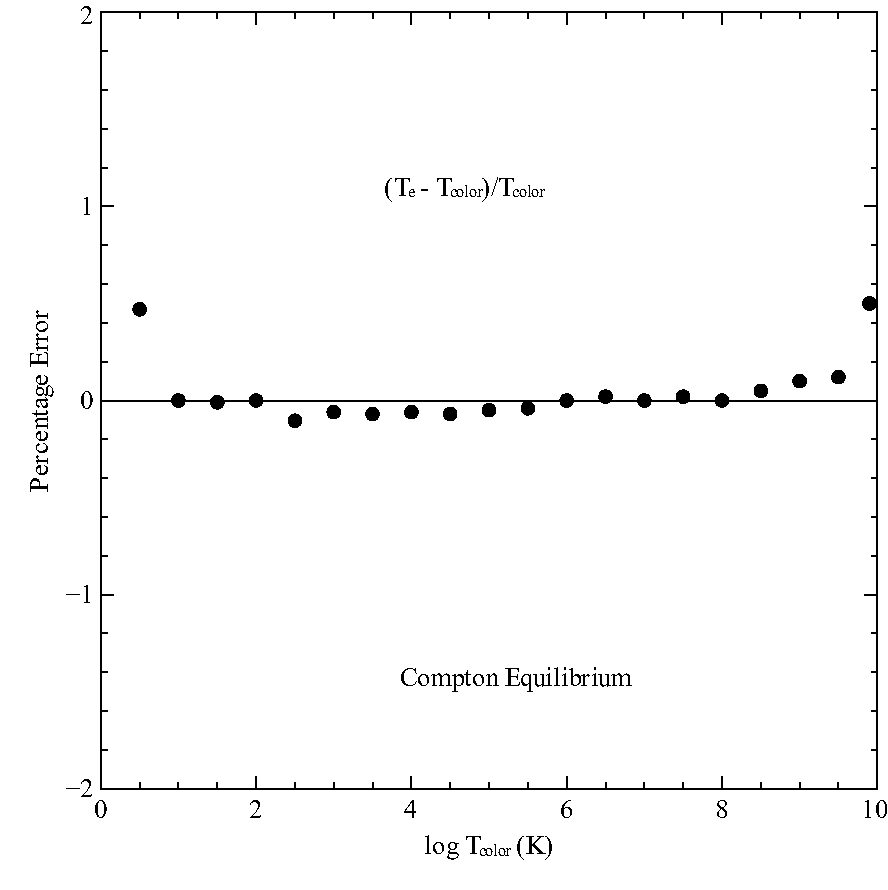
\includegraphics[scale=0.7]{ComptonEquilibriumError}
\caption[Compton Equilibrium Error]{Thermal equilibrium in the Compton Limit. Calculations are for
blackbody continua of various temperatures, given as $T_{color}$ along the x-axis.
The energy density temperature $T_u$ is set equal to $T_{color}$.  The density is
adjusted to maintain ionization parameters $U\sim  10^{10}$, so that the thermal
equilibrium equations are dominated by the Compton exchange problem.  The
deviation of the computed equilibrium temperature $T_e$ from the asymptotic
Compton temperature $T_{color}$ is shown.}
\end{figure}

The intended temperature range of validity for \Cloudy\ is \TEMPLIMITLOW $ -$\TEMPLIMITHIGH.  Over the more limited range $10 \K - 10^9 \K$ the computed Compton
 temperature, for conditions in which strict TE is expected, is generally
equal to the color temperature within three significant figures
(see Figure \ref{fig:ComptonEquilibriumError}).
At temperatures much greater than 10$^9$ K the electrons become
relativistic; \Cloudy\ is not intended for these conditions.  For temperatures
much less than 10 K the computed temperature fails high because the energy
bandwidth of the continuum array does not extend
below \emm .
As
a further test, the models presented by \citep{Krolik1981}
were recomputed with excellent agreement (typically within 3\%) with their
computed Compton temperatures.

For a blackbody radiation field with $T_u \ne T_{color}$ the Compton temperature
will not be equal to $_{Tcolor}$ because induced scattering will not contribute
the required amount of heating-cooling.  This case is shown in Figure
\ref{fig:ComptonSTE},
the results of a series of calculations in which the energy density
temperature was varied (this is shown as the x-axis), but the color
temperature held fixed at 10$^5$~K.

\begin{figure}
\centering
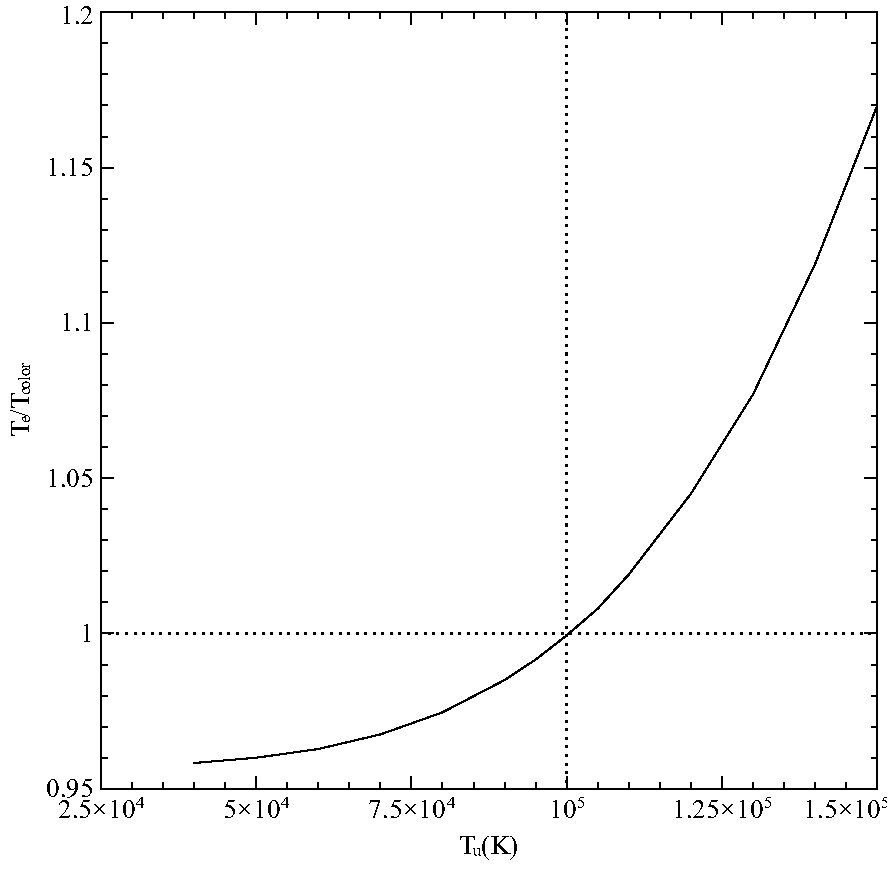
\includegraphics[scale=0.75]{ComptonSTE}
\label{fig:ComptonSTE}
\caption[Compton equilibrium in the STE limit]{Calculations are for 10$^5$ K blackbodies and various values of the
energy density temperature $T_u$, indicated along the x-axis. The ratio of
the computed equilibrium temperature $T_e$ to the color temperature
$T_{color}$
is shown.  The two are equal when the energy density and color temperatures
are equal. cmpnlte}
\end{figure}

Note also that when $T_u > T_{color}$ induced Compton heating
drives $T_e$ above $T_{color}$.
Only when the color and energy density temperatures are equal
do the equilibrium and color temperatures match.

\section{Bound Compton ionization, heating}

Compton scattering can ionize atoms for photons of sufficiently high
energy ($\approx 2.3$ keV for hydrogen).  The energy given to an electron
by a 90$^{\circ}$
scattering is found by rearranging equation \ref{eqn:ComptonEnergyShift}above
\begin{equation}
e = h\nu \left( {1 - \frac{1}{{1 + \frac{{h\nu }}{{m{c^2}}}}}} \right).
\end{equation}
Setting this equal to the ionization potential of the species, $h{\nu _o}$,
electrons will be removed by photons having an energy greater than
\begin{equation}
h\nu  = \sqrt {h{\nu _o}m{c^2}}.
\end{equation}

\section{Expansion cooling }

Adiabatic cooling (erg cm$^{-3}$ s$^{-1}$) due to the hydrodynamic expansion of
the gas is given by
\begin{equation}
{L_{\rm exp}} =  - \frac{{DU}}{{Dt}} =  - \frac{p}{\rho }\frac{{D\rho
}}{{Dt}} + U\nabla  \cdot {\bf{v}} = -{5\over2} kT\frac{{dn}}{{dt}} 
= -{5\over2}nkT\left[
{\frac{a}{u} + \frac{{2u}}{r}} \right]\quad [\mathrm{erg~s}^{-1} \mathrm{cm}^{-3}]
\end{equation}
where $n, a, u$, and $r$ are the total particle density, acceleration,
wind velocity, and radius respectively.  This cooling term is only
included when a wind geometry.  

It should be noted that in this case, a quasi-static assumption is
being made, so the results are only valid so long as all
heating/cooling and ionization timescales are much shorter than the
dynamical timescale.  

Where this is not the case, the expansion cooling needs to be treated
by an explicit time dependent approach, as detailed in the time
dependent flow section.

\section{Free-free heating-cooling}

The volume free-free heating rate is given by
\begin{equation}
{G_{ff}} = 4\pi \int_{{\nu _c}}^\infty  {{n_e}\,{\alpha _\nu }\left( {ff}
\right)\;{J_\nu }\;d\nu } [\mathrm{erg~s}^{-1} \mathrm{cm}^{-3}]
\end{equation}
where the free-free cross section is denoted by $\alpha_\nu(ff)$ and $\nu_c$ is the critical
frequency defined below, and $J_{\nu}$ is the sum of the attenuated incident
radiation field and the OTS line fields.  Diffuse reemission, mainly
free-free emission, \emph{is not} included in this integral, as discussed below.

The code works with the difference between cooling and heating, since
this is numerically more stable than considering each term as an independent
heat source or coolant.

Cooling due to diffuse continua are treated by defining a critical
frequency $\nu_c$ as follows.  Gas at a depth $r$ into the cloud is transparent
to photons with energies above a critical frequency $\nu_c$ such that
\begin{equation}
{\tau _c} = \int_0^r {\kappa \left( {{\nu _c}} \right)\;\,f\left( r
\right)\,dr}  = \int_0^r {{\alpha _\nu }} \left( {ff,\,{\nu _c}}
\right){n_e}\,f\left( r \right)\,dr = 1
\end{equation}
and optically thick at lower frequencies.
The critical frequency $\nu_c$ is
evaluated for each zone.

The free-free cooling rate is then given by
\begin{equation}
{\Lambda _{ff}}\left( \tau  \right) = \int_{{\nu _c}}^\infty  {{n_e}{\alpha
_\nu }(ff)\;4\pi \,{B_\nu }\left( {{T_e}} \right)\;d\nu  = {\Lambda _{ff}}(0)
\times \exp \left( { - h{\nu _c}/kT} \right)}
\end{equation}
where $\Lambda_{ff}(0)$ is the optically thin cooling rate and $B_\nu (T)$ is Planck's
function.  This is equivalent to assuming that, for $\nu < c$, where the cloud
is optically thick, free-free heating and cooling exactly balance, as
suggested by Kirchhoff's law and detailed balance considerations.   Energies
below $\nu_c$ are not included in free-free heating or cooling.  This critical
frequency is not allowed to be less than the plasma frequency for the current
conditions.

\section{Photoelectric heating, recombination cooling}

The net heating rate due to photoelectric heating less spontaneous and
induced recombination cooling of level $n$ is given by
\begin{equation}
G = {G_{n,\;\kappa }} - {\Lambda _{ind,\;n}} - {\Lambda _{spon,\;n}}\quad
[\mathrm{erg~s}^{-1} \mathrm{cm}^{-3}]
\end{equation}
where the volume heating rate due to photoionization is
\begin{equation}
{G_{n,\;\kappa }} = {n_n}\int_{{\nu _o}}^\infty  {\frac{{4\pi {J_\nu
}}}{{h\nu }}\;{\alpha _\nu }\;h\left( {\nu  - {\nu _o}} \right)\;d\nu }
\quad [\mathrm{erg~s}^{-1} \mathrm{cm}^{-3}],
\end{equation}
the volume cooling rate due to induced recombination is
\begin{equation}
{L_{ind,\;n}} = {n_e}{n_p}\;4\pi \;P_n^*\int_{{\nu _o}}^\infty
{\frac{{{J_\nu }}}{{h\nu }}\;{\alpha _\nu }\exp \left( { - h\nu /kT}
\right)\;h\left( {\nu  - {\nu _o}} \right)\;d\nu }
\quad [\mathrm{erg~s}^{-1}\mathrm{cm}^{-3}]
\end{equation}
and the cooling rate due to spontaneous radiative recombination is
\begin{equation}
{L_{spon,\;n}} = {n_e}{n_p}kT\beta \left( {T,n} \right)\quad
[\mathrm{erg~s}^{-1} \mathrm{cm}^{-3}] .
\end{equation}
The cooling rate coefficient $\beta(T,n)$ is evaluated as described
elsewhere in this document.

\section{Collisional ionization---three-body recombination}

The net volume-heating rate due to collisional ionization less three-body
recombination is given by
\begin{equation}
{G_{n,\kappa }} - {L_{n,\kappa }} = \sum\limits_n
{P_n^*{n_e}{n_p}{C_{n,\kappa }}\;h{\nu _o}\;\left( {1 - {b_n}} \right)}
\quad [\mathrm{erg~s}^{-1} \mathrm{cm}^{-3}]
\end{equation}
where $C_{n,\kappa}$ is the collisional ionization rate, $P*$ are STE populations, and
$b_n$ is the departure coefficient.  The term $(1 - b_n)$ is only large and
positive for very low levels, in which $I_n > kT$.  Far from thermodynamic
equilibrium this is usually a net cooling process only for the ground term.
This is because departure coefficients for excited states are nearly unity
while the ground level usually has $b_n\cong 1$.

\section{H$^-$ heating and cooling}

\subsubsection{H$^-$ bound-free}

The volume-heating rate due to spontaneous absorption (photodissociation)
is
\begin{equation}
{G_{{H^ - }}} = n({H^ - })\;\int_{{\nu _o}}^\infty  {\frac{{4\pi {J_\nu
}}}{{h\nu }}} \;{\alpha _\nu }\;h\left( {\nu  - {\nu _o}} \right)\;d\nu
\quad [\mathrm{erg~s}^{-1} \mathrm{cm}^{-3}]
\end{equation}
where symbols have their usual meaning.  The volume-cooling rate due to
induced radiative attachment is
\begin{equation}
{L_{ind,\;{H^ - }}} = {n_e}{n_{{H^o}}}\;{P^*}({H^ - })\int_{{\nu
_o}}^\infty  {{\alpha _\nu }\;\frac{{4\pi {J_\nu }}}{{h\nu }}\exp \left(
{ - h\nu /kT} \right)\;h\left( {\nu  - {\nu _o}} \right)\;d\nu }
\quad [\mathrm{erg~s}^{-1} \mathrm{cm}^{-3}]
\end{equation}
while the volume cooling rate for spontaneous radiative attachment is
\begin{equation}
{L_{spon,\;{H^ - }}} = {n_e}{n_{{H^o}}}8\pi \;{P^*}({H^ - })\int_{{\nu
_o}}^\infty  {{\alpha _\nu }\;\frac{{{\nu ^2}}}{{{c^2}}}\;\exp \left( {
- h\nu /kT} \right)\;h\left( {\nu  - {\nu _o}} \right)\;d\nu }
\quad [\mathrm{erg~s}^{-1} \mathrm{cm}^{-3}].
\end{equation}

\subsection{H$^-$ free-free}

Free-free heating and cooling by H$^-$ is also significant, although less
so than bound-free heating.  This is included, making the appropriate
correction for stimulated emission, using the cross sections given by
\citep{Vernazza1981}.

Under most circumstances H$^-$ bound-free heating and cooling are much more
important than H$^-$ free-free processes.  This is surprising at first sight,
since standard opacity curves comparing bound-free and free-free opacities
(Bates et al. 1975; \citealp{Mihalas1978}) show that the two are comparable.  These
curves are for strict thermodynamic equilibrium, with H$^-$ departure
coefficients of unity.  Like the ground state of hydrogen, the departure
coefficient for H$^-$ is often many orders of magnitude larger than unity,
so that the H$^-$ bound-free opacity and the resulting heating greatly exceed
the H$^-$ free-free opacity.

\section{Line heating and cooling }

\subsection{Overview}

All lines will be treated as data types \cdTerm{EmLine}.  The following sections
describe the major routines for computing heating and cooling for $n$-level
atoms. Emission lines are often optically thick.  All lines are transferred
using escape probabilities, by determining level populations including both
collisional and radiative processes (see, for example, \citealp{Elitzur1992}).  Line
masing can sometimes occur, and again is treated using escape probabilities.

In all cases the net cooling due to a transition is given as
\begin{equation}
{L_{line}} = h{\nu _{u,l}}\left( {{n_l}{C_{l,u}} - {n_u}{C_{u,l}}} \right)
\quad [\mathrm{erg~cm}^{-3} \mathrm{s}^{-1}]
\end{equation}
where the populations of levels are given by $n_i$ and $C_{ij}$ is the collision
rate.  This cooling is evaluated in a series of routines
which are responsible for evaluating the line intensity,
cooling, and destruction rate, and entering these into the appropriate
stacks.  Each routine sets the following attributes.

Lines can act to \emph{heat} rather than cool the gas when the gas is irradiated
by a continuum with a brightness temperature greater than the gas temperature
at the line energy. This is an important gas heating mechanism for PDRs,
for instance \citep{Tielens1985a}.  If $\eta$ is the photon occupation
number of the attenuated incident continuum at the line frequency, then
the rate atoms are excited from the ground level is given by
$\eta\varepsilon A_{ul}$ where
$\varepsilon $ is the line escape probability.  A fraction $C_{ul}/(C_{ul}+
\varepsilon A_{ul})$ of these
radiative excitations is converted into heat by collisional de-excitation.
The net heating due to this process is then
\begin{equation}
{G_{FIR}} = {n_l}\,{\eta _\nu }\,{\varepsilon _{lu}}\,{A_{ul}}\left(
{\frac{{{C_{ul}}}}{{{C_{ul}} + {\varepsilon _{lu}}\,{A_{ul}}}}} \right)\,h\nu
\quad [\mathrm{erg~cm}^{-3} \mathrm{s}^{-1}]
\end{equation}
where $n_l$ is the density of the ground level.  This process is included for
all transferred lines.

\subsection{Two level atoms}

Cooling due to collisional excitation of two level atoms of the heavy
elements is evaluated in routine \cdTerm{level2}.  This routine does the following:
a) finds the abundance of the two levels by balancing collisional and
radiative processes, subject to the sum $n_l +n_u =$ abundance.  b) adds the
line cooling (or heating) to the total cooling, c) adds the line derivative
to $dC/dT,$ d) evaluates the fraction of the escaping line destroyed by
background opacity, e) adds this to the local OTS radiation field, f) records
the line opacity population $n_l-n_u g_l/g_u$.  The populations of the atom are
saved in the vector \cdTerm{PopLevls}.

\subsection{Three level atoms}

The level populations, cooling, and line destruction by background opacity
sources are computed for three level atoms in routine \cdTerm{level3}.

Routine \cdTerm{level3} is called with three arguments, the three line structures.
Levels are designated by the indices 0, 1, and 2, with 0 being the lowest
level.  The routine is called with three line structures, indicated by $t10$,
$t21$, and $t20$, each representing the downward radiative transition between
the indicated levels.  Any one of these transitions may be a dummy
transition, using the dummy line \emph{TauDmmy} provided for this purpose.  The
total rates between any two levels $i\Lambda j$ is indicated by $R_{ij}$.  This includes
collisions, radiative decays (both photon escape and destruction by
background opacity), and induced transitions.  If the total abundance of
the parent ion is A, the three balance equations are
\begin{equation}
{n_0} + {n_1} + {n_2} = A
\end{equation}
\begin{equation}
{n_0}\left( {{R_{01}} + {R_{02}}} \right) = {n_1}{R_{10}} + {n_2}{R_{20}}
\end{equation}
\begin{equation}
{n_1}\left( {{R_{10}} + {R_{12}}} \right) = {n_2}{R_{21}} + {n_0}{R_{01}}.
\end{equation}
Setting $n_0$ to $A-n_1-n_2$ the above becomes
\begin{equation}
\left( {{R_{01}} + {R_{02}}} \right)\left( {A - {n_1} - {n_2}} \right)
= {n_1}{R_{10}} + {n_2}{R_{20}}.
\end{equation}
After gathering terms this equation becomes
\begin{equation}
A\left( {{R_{01}} + {R_{02}}} \right) = {n_1}\left( {{R_{10}} + {R_{01}}
+ {R_{02}}} \right) + n_2^{}\left( {{R_{20}} + {R_{01}} + {R_{02}}} \right) .
\end{equation}
Substituting for $n_0$ we find
\begin{equation}
{n_1}\left( {{R_{10}} + {R_{12}}} \right) = {n_2}{R_{21}} + {R_{01}}\left(
{A - {n_1} - {n_2}} \right).
\end{equation}
Gathering terms this equation becomes
\begin{equation}
{n_1}\left( {{R_{10}} + {R_{12}} + {R_{01}}} \right) = A{R_{01}} +
{n_2}\left( {{R_{21}} - {R_{01}}} \right)
.
\end{equation}
Solving we obtain
\begin{equation}
{n_1} = \frac{{A\left( {{R_{01}} + {R_{02}}} \right)}}{{{R_{10}} + {R_{01}}
+ {R_{02}}}} - \frac{{{n_2}\left( {{R_{20}} + {R_{01}} + {R_{02}}}
\right)}}{{{R_{10}} + {R_{01}} + {R_{02}}}}
\end{equation}
and we find
\begin{equation}
{n_1} = \frac{{A{R_{01}}}}{{{R_{10}} + {R_{12}} + {R_{01}}}} +
\frac{{{n_2}\left( {{R_{21}} - {R_{01}}} \right)}}{{{R_{10}} + {R_{12}}
+ {R_{01}}}}
\end{equation}
Equating the two and gathering terms we obtain
\begin{equation}
{n_2}\left( {\frac{{{R_{21}} - {R_{01}}}}{{{R_{10}} + {R_{12}} + {R_{01}}}}
+ \frac{{{R_{20}} + {R_{01}} + {R_{02}}}}{{{R_{10}} + {R_{01}} + {R_{02}}}}}
\right) = \frac{{A\left( {R_{01}^{} + {R_{02}}} \right)}}{{{R_{10}} +
{R_{01}} + {R_{02}}}} - \frac{{A{R_{01}}}}{{{R_{10}} + {R_{12}} +
{R_{01}}}}
\end{equation}
with the solution
\begin{equation}
{n_2} = A{\raise0.7ex\hbox{${\left( {\frac{{\left( {R_{01}^{} + {R_{02}}}
\right)}}{{{R_{10}} + {R_{01}} + {R_{02}}}} - \frac{{{R_{01}}}}{{{R_{10}}
+ {R_{12}} + {R_{01}}}}} \right)}$} \!\mathord{\left/
 {\vphantom {{\left( {\frac{{\left( {R_{01}^{} + {R_{02}}}
\right)}}{{{R_{10}} + {R_{01}} + {R_{02}}}} - \frac{{{R_{01}}}}{{{R_{10}}
+ {R_{12}} + {R_{01}}}}} \right)} {\left( {\frac{{{R_{21}} -
{R_{01}}}}{{{R_{10}} + {R_{12}} + {R_{01}}}} + \frac{{{R_{20}} + {R_{01}}
+ {R_{02}}}}{{{R_{10}} + {R_{01}} + {R_{02}}}}}
\right)}}}\right.\kern-\nulldelimiterspace}
\!\lower0.7ex\hbox{${\left( {\frac{{{R_{21}} - {R_{01}}}}{{{R_{10}} +
{R_{12}} + {R_{01}}}} + \frac{{{R_{20}} + {R_{01}} + {R_{02}}}}{{{R_{10}}
+ {R_{01}} + {R_{02}}}}} \right)}$}}
.
\end{equation}
In the code the term in the numerator in the previous equation is called
\emph{alpha}, and the denominator \emph{beta}.
Replacing n2 in the above we obtain
\begin{equation}
{n_1} = {\raise0.7ex\hbox{${\left[ {A\left( {{R_{01}} + {R_{02}}} \right)
- {n_2}\left( {{R_{20}} + {R_{01}} + {R_{02}}} \right)} \right]}$}
\!\mathord{\left/
 {\vphantom {{\left[ {A\left( {{R_{01}} + {R_{02}}} \right) - {n_2}\left(
{{R_{20}} + {R_{01}} + {R_{02}}} \right)} \right]} {\left( {{R_{10}} +
{R_{01}} + {R_{02}}} \right)}}}\right.\kern-\nulldelimiterspace}
\!\lower0.7ex\hbox{${\left( {{R_{10}} + {R_{01}} + {R_{02}}} \right)}$}} .
\end{equation}
Again the two terms are called \emph{alpha} and \emph{beta}.

\subsection{Li Sequence}

Table \ref{tab:LiSequence} gives the stronger lines of Li-sequence ions.   \cdTerm{Level3} is used for this sequence.

\begin{table}
\caption{Lithium Sequence Lines }
\label{tab:LiSequence}
\begin{tabular}{llllll}
\hline
N& Ion& $j=3/2-1/2$& $j=1/2-1/2$& $j=3/2-1/2$& $j=1/2-1/2$\\
\hline
6& C IV& 1548.195& 1550.770& 312.422& 312.453\\
7& N V&  1238.821& 1242.804& 209.2702& 09.303\\
8& O VI& 1031.9261& 1037.6167& 150.088& 150.124\\
10& Ne VIII& 770.409& 780.324& 88.134\\
12& Mg X& 609.79& 624.95& 57.88& 57.92\\
13& Al XI& 550.03& 568.15& 48.30& 48.34\\
14& Si XII& 499.40& 520.67& 40.92\\
16& S XIV& 417.61& 445.77& 30.43\\
18& Ar XVI& 353.92& 389.14& 25.53\\
20& Ca XVIII& 302.215& 344.772& 18.69& 18.73\\
26& Fe XXIV& 192.017& 255.090& 10.62& 10.66\\
\hline
\end{tabular}
\end{table}

\subsection{Boron Sequence}

Figure \ref{fig:AtomBoronSequence} shows levels within
the lowest three configurations of the Boron
sequence.

\begin{figure}
\centering
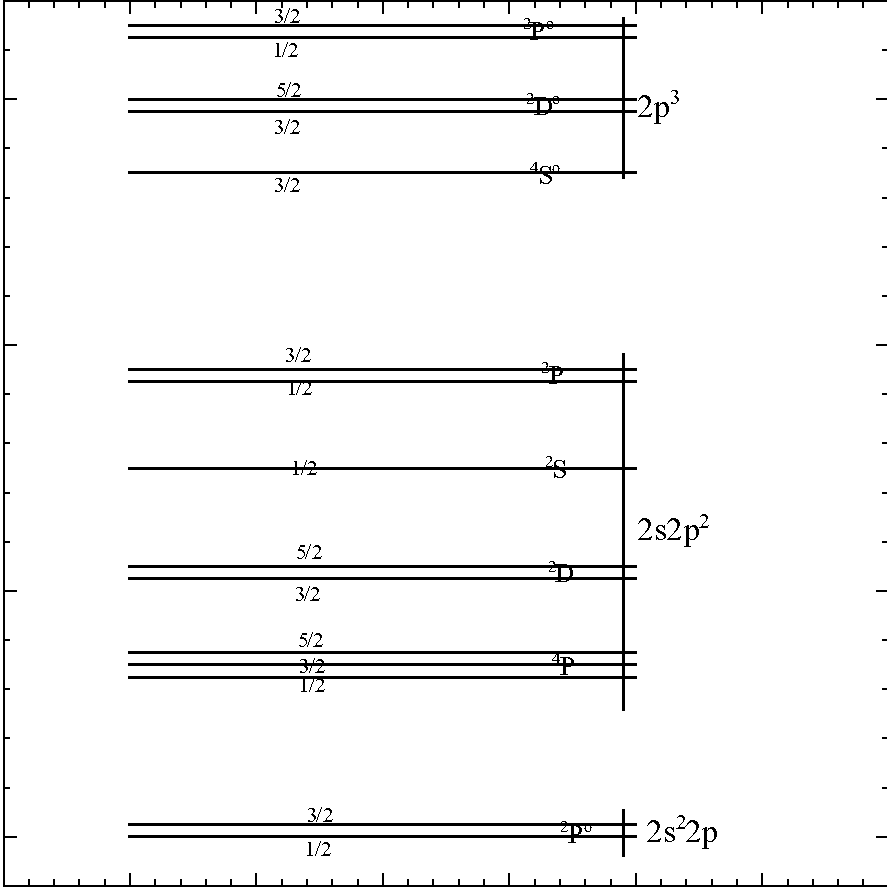
\includegraphics[scale=0.6]{AtomBoronSequence}
\label{fig:AtomBoronSequence}
\caption{Energy Level Diagram for Boron Sequence.}
\end{figure}

\subsection{Beryllium sequence atoms}

Figure \ref{fig:AtomBeSequence} shows the model of the Beryllium sequence.
The level populations, cooling, and line destruction by background opacity
sources are computed for a specialized four level atom in routine
\cdTerm{AtomSeqBeryllium}.

\begin{figure}
\centering
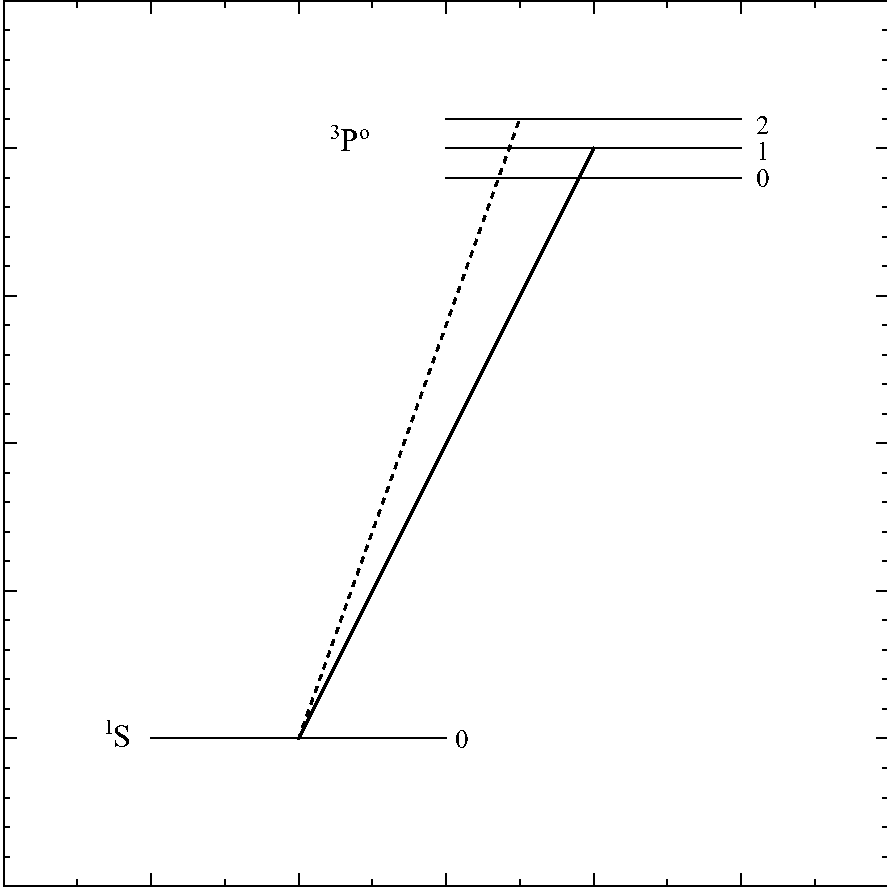
\includegraphics[scale=0.5]{AtomBeSequence}
\label{fig:AtomBeSequence}
\caption{Energy Level Diagram for Beryllium Sequence.}
\end{figure}

Routine \cdTerm{beseq} is called with five arguments, the collision strengths
between the excited triplet levels, the line optical depth array for the
fast $(j=1$ to $j=0)$ transition, and the transition probability for the slow
$(j=2$ to $j=0)$ transition. Induced processes are only included for the fast
transition.   The collision strength stored in the line array is the
collision strength for the entire multiplet.  Rates to levels within the
term are assumed to scale as the ratio of level statistical weight to term
statistical weight.  The level populations for the ground and excited states,
with no correction for stimulated emission, are returned in the array
\cdTerm{PopLevls}, contained in the common block of the same name.

The total rates between any two levels $i\Lambda j$
is indicated by $R_{ij}$.  This
includes collisions, radiative decays (for the fast transition, both photon
escape and destruction by background opacity, and induced transitions).
If the total abundance of the parent ion is $A$, the three balance equations
are
\begin{equation}
{n_0} + {n_1} + {n_2} + {n_3} = A
\end{equation}
\begin{equation}
{n_0}\left( {{R_{01}} + {R_{02}} + {R_{03}}} \right) = {n_1}{R_{10}} +
{n_2}{R_{20}} + {n_3}{R_{30}}
\end{equation}
\begin{equation}
{n_1}\left( {{R_{10}} + {R_{12}} + {R_{13}}} \right) = {n_3}{R_{31}} +
{n_2}{R_{21}} + {n_0}{R_{01}}.
\end{equation}
\begin{equation}
{n_2}\left( {{R_{20}} + {R_{21}} + {R_{23}}} \right) = {n_3}{R_{32}} +
{n_1}{R_{12}} + {n_0}{R_{02}} .
\end{equation}
Collisions are included in all these terms.  $R_{32}$ includes the slow downward
line escape, while $R_{02}$ and $R_{20}$ includes escape, destruction by background
opacity, and fluorescent excitation---deexcitation.  In the code the terms
on the LHS of equations 39, 40, and 38 are called $\alpha$, $\beta$,
and~$\gamma$.

\section{Evaluation of the cooling function}

\subsection{Total cooling}

The cooling function is evaluated in routine \cdTerm{coolr}.  This in turn calls
other routines which compute cooling for individual elements.  Each
individual coolant is entered as a separate quantity in the array
\cdTerm{cooling}.
Under some extreme circumstances agents that are normally coolants can
actually heat the gas.  Negative coolants are stored in a parallel array,
\cdTerm{heatnt}.

The total cooling is the sum of this array, referred to as the variable
\cdTerm{ctot}, and evaluated in routine \cdTerm{SumCool}.

\subsection{The cooling derivative}

As the cooling is evaluated, its approximate temperature derivative is
computed by making analytic expansions of the cooling for individual agents.
For instance, collisionally excited lines of positive ions have collisional
excitation rates that depend on the product
\begin{equation}
{L_{line}} \propto {n_e}{n_{ion}}T_e^{ - 1/2}\exp ( - {T_{exc}}/{T_e})
\end{equation}
where $T_{exc}$ is the excitation temperature of the line.  In this case the
derivative of the cooling function can be expressed as
\begin{equation}
\frac{{d{L_{line}}}}{{dT}} \propto {n_e}{n_{ion}}\frac{d}{{d{T_e}}}T_e^{
- 1/2}\exp ( - {T_{exc}}/{T_e}) = {L_{line}}\left[
{\frac{{{T_{exc}}}}{{T_e^2}} - \frac{1}{{2{T_e}}}} \right]
\end{equation}
This derivative is used by the thermal predictor-corrector routine to make
the initial guess at a new temperature.  This is approximate since both
electron and ionic densities also depend on the temperature.

\section{Evaluation of the heating function}

Various contributions to the heating function are evaluated throughout
the code.  Each heating agent stores its contribution to the total heating
within a cell of the two dimensional array \emph{heating}.   The total heating
is always the sum of the total contents of the \emph{heating} array.

\section{Equilibrium calculations}

This is largely taken after \citet{Ferland1988}.

\subsection{Hydrogen only}

Figure \ref{fig:HydrogenRadiationSTE} shows the results of a series of calculations in which the full
set of statistical and thermal equilibrium equations are solved for thin
cells of pure hydrogen gas with various densities.

\begin{figure}
\centering
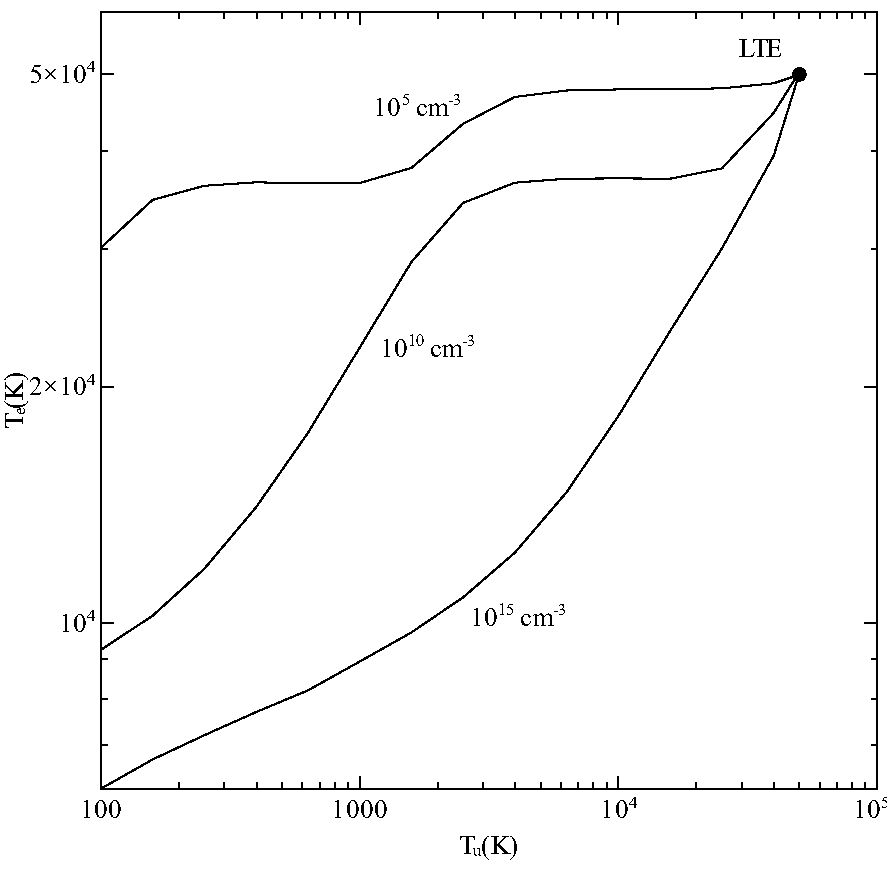
\includegraphics[scale=0.9]{HydrogenRadiationSTE}
\label{fig:HydrogenRadiationSTE}
\caption[Pure hydrogen approach to STE]{Thermal equilibrium calculations for an optically thin gas with
3 hydrogen densities are shown as a function of the radiation field energy
density, parameterized as $T_u$.  Ionization is by a $5 \times 10^4$ K black body.
Various processes drive the gas to thermodynamic equilibrium when $T_u$ reaches
$5\times 10^4$~K.}
\end{figure}

The ionizing continuum is, in all cases,
a black body with $T_{color} = 5\times 10^4 \K$,
and the energy density of the radiation field is varied, up to the
thermodynamic equilibrium limit, $T_u = T_{color}$.

Although the gas temperature in the thermodynamic equilibrium limit does
not depend on the gas density, the physical processes that drive the gas
to this temperature do.  Thermal equilibrium calculations were performed
with three densities chosen to span a fairly wide range.  For low densities
$(n(H) = 10^5$~cm$^{-3}$) the gas remains highly ionized for all values of
$T_u$ shown.
The temperature in thermodynamic equilibrium is set by the balance between
Compton and inverse-Compton scattering.  The intermediate density case $(n(H)
= 10^{10}$ cm$^{-3}$) reaches thermodynamic equilibrium with $\sim$3/4 of the
heating-cooling set by Compton scattering and the remainder due to free-free
and free-bound processes.  The high-density $(n(H) = 10^{15}$ cm$^{-3}$) case reaches
its thermodynamic equilibrium temperature with a balance between free-free
(1/3 of the total) and free-bound (2/3 of the total) processes.  In all
cases the level populations and electron temperature are within $\sim$1\% of their
expected thermodynamic equilibrium values when $T_u = T_{color}$.

\subsection{Helium-only gas}

To do \dots.

\subsection{Metal rich gas}

Simulations of very metal rich gas has been a major emphasis of the code
as described by \citep{Hamann1993} and
\citep{Ferland1996}.  In these cases the thermal
and ionization balance is totally dominated by the heavy elements.

Figure \ref{fig:HighMetalsLTE} shows the results of a series of calculations in which gas with
strongly enhanced abundances of the heavy elements is exposed to a series
of black body radiation fields with different temperatures and energy
densities.   \citep{Ferland1988} and \citep{Ferland1989} gave
analogous calculations for pure hydrogen clouds.  The filled circles
represent the cases where the energy densities of the radiation field are
equal to the color temperature, and strict thermodynamic equilibrium is
expected.  This is indeed the case.  The distribution of ionization for
each color temperature is radically different, but the line interactions
with the radiation field bring the gas to the expected equilibrium
temperature.  This tests both the ionization and thermal balance in this
extreme environment.

\begin{figure}
\centering
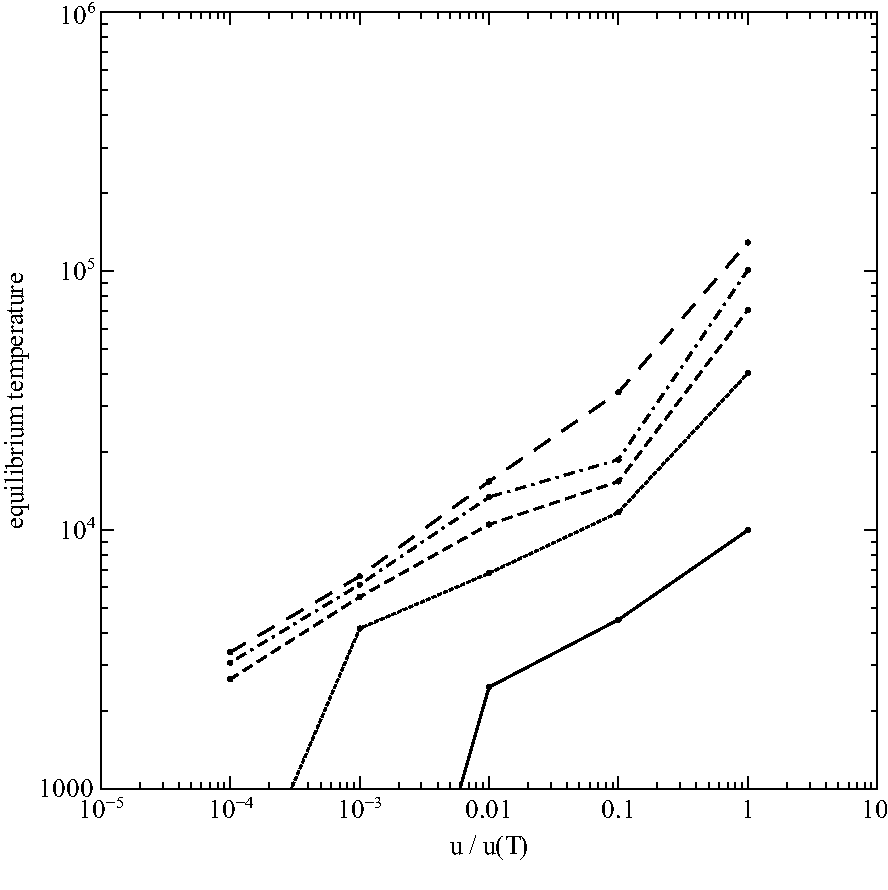
\includegraphics[scale=0.9]{HighMetalsLTE}
\label{fig:HighMetalsLTE}
\caption[High metallicity gas approach to LTE]
{Equilibrium temperature of gas exposed to five black bodies with
various energy density temperatures.  The color temperatures of the
blackbodies are 10000 K, 40000 K, 70000 K, 100000 K and 130000 K.  The
metallicity was 10 times solar (Hamann and Ferland 1993) so that heating
cooling of thousands of heavy element emission lines dominates the thermal
equilibrium.  The simulation is of an optically thin cell of gas with density
$10^{10}$ cm$^{-3}$ (results do not depend on this density).  The x-axis is the local
energy density relative to the energy density in thermodynamic equilibrium
at that temperature.  The gas goes to thermodynamic equilibrium when the
radiation field does (the color and energy density temperatures are equal).}
\end{figure}

   %proof 1
\chapter{GRAIN PHYSICS}
% !TEX root = hazy3.tex

\section{Overview}

The following discussion outlines some physical processes relating to
grains, as incorporated in \Cloudy.  It is adopted from \citet{Baldwin1991},
and was written in close collaboration with P.G. Martin.

Much of this physics has been updated to that described by \citet{VanHoof2004}, which is based on \citep{Weingartner2001a}.

Several grain populations, types of graphite and ``astronomical
silicates'', are available.  Usually one of each type, for a total of two,
is selected, although there is no limit to the number of grain populations.
Optical properties like opacity of the species are based on a realistic
power-law size distribution.  Other properties (like potential and
temperature) are computed for a mean grain size rather than calculated for
each individual size.

 The following describes the ``old'', default, grains that were originally
incorporated into the code in the late 1980's (\citealp{Baldwin1991}).  These
use optical properties that correspond to averages over the grain size
distribution.  The current treatment both resolves the grain
size distribution and includes single photon heating for the smaller grains.
This new treatment is described in \citet{VanHoof2001} and will be
included in this document at a later time.

\section{Grain opacity}

Grains are not included in the calculation by default.  When enabled
with the grain command the default mixture has interstellar medium (ISM)
properties.  Grains more similar to those seen in Orion or planetary nebulae
are also available.

\subsection{ISM grains}

The optical constants for the default (ISM) grain species are from the
calculations of \citep{Martin1990}.  These extend the work of
\citep{Draine1984} to ionizing energies where the grains are strongly absorbing.
These opacity calculations were based on the
\citep{Mathis1977} power-law size distribution to simulate interstellar extinction in
diffuse clouds.

\subsection{Orion grains}

Grains within the Orion Nebula have a relatively large ratio of total
to selective extinction $R$ and an exceptionally gray opacity in the
ultraviolet.  These are both indicative of a deficiency in small grains
and a larger mean grain size.  To account for this, a second set of opacity
functions is included, the Orion group.  For this the value of the smallest
size (a$_-$) in the \citep{Mathis1977} size distribution was increased from
0.0025$\mu$m to 0.03$\mu$m.  While this simple adjustment of the size distribution
is not entirely adequate for explaining the details of the visible and near
ultraviolet Orion extinction curve \citep{Mathis1981}, it should
be an improvement for the ionizing ultraviolet portion, which is most
important.

The Orion extinction curve is designed to simulate the large R grains
observed in this H~II region.  Relative to ISM standard grains the total
amount of grain material was preserved, so that $\alpha_{\mathrm{abs}}$ in the infrared and
in the EUV and X-Ray regions remains unchanged.  The main differential effect
is to lower the cross section through a broad peak at 1 Ryd.

\subsection{PN grains}

Infrared opacities for the silicate component are taken from unpublished
work by K. Volk.  Ultraviolet silicate cross sections, and the graphite
constituent, are standard ISM.

\subsection{Extinction}

The ISM extinction properties, both effective scattering (subscript scat)
and absorption (subscript abs), are shown in Figure~\ref{fig:GrainOpacity}.

\begin{figure}
\centering
\label{fig:GrainOpacity}
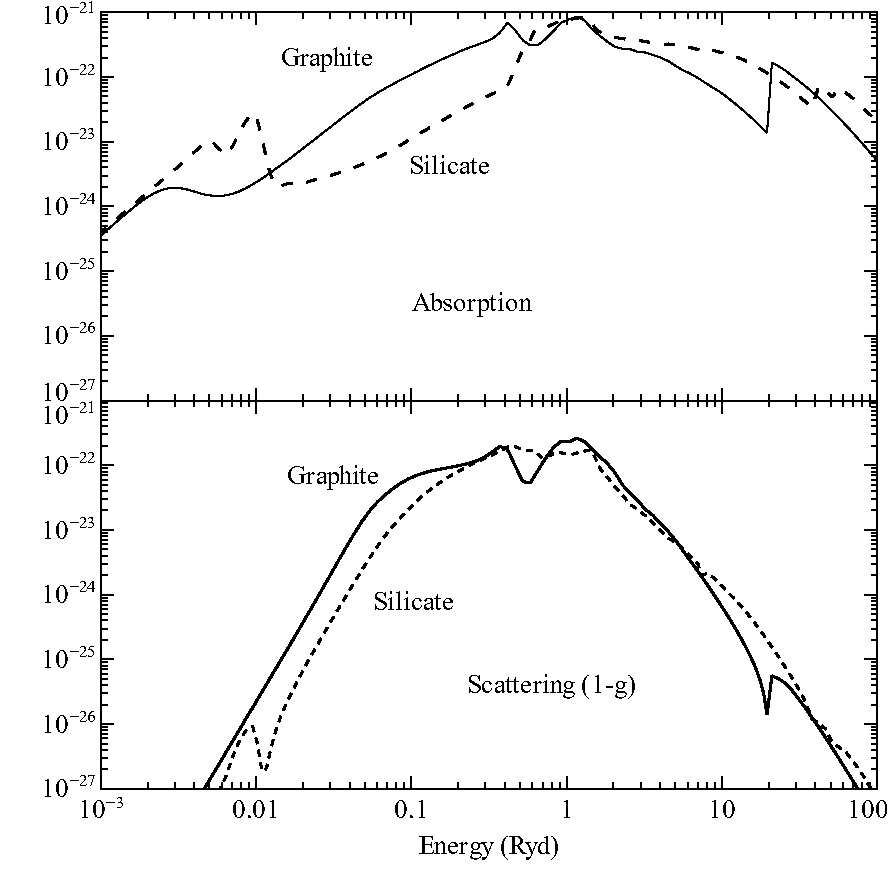
\includegraphics{GrainOpacity}
\caption[Grain opacities]{The absorption and scattering cross sections (cm$^2$ per hydrogen
nucleon) for the two ISM grain populations, graphite and silicate, are shown.
The effective scattering cross section is the scattering cross section
multiplied by $1-g$, where $g$ is the asymmetry parameter.}
\end{figure}

The quantities plotted are cross sections (cm$^2$) per H nucleon:
$\sigma = \kappa/n(H)$,
where $\kappa$ (cm$^{-1}$) is the opacity due to grains and $n(H)$
(cm$^{-3}$) is the local
density of H in any form.  Rather than the total scattering cross section
$\sigma_s$ an effective scattering cross section $\sigma_{scat} = \sigma_s
(1-g)$ is plotted.  This
discounts the radiation scattered near the forward direction.  The asymmetry
parameter $g$ approaches unity at high and low energies, particularly for
larger grains, so that $\sigma_{scat}$ becomes much less than $\alpha_{abs}$

The optical depth $\tau$ is $\sigma$ times the hydrogen column density
(or $\kappa$ integrated
over the path).  Absorption attenuates the incident radiation field as
exp($-\tau_{abs}$).  The effects of scattering are more difficult to model.  In an
open geometry, scattering attenuates approximately as
$(1+0.5 \tau_{scat})^{-1}$.
However, in a closed geometry, to within factors of order unity, the
scattered light is not lost from the beam, and the scattering opacity can
be ignored.  In either case, effective grain scattering optical depth is
generally fairly small through the ionized nebula at ionizing energies.

\section{Photoelectric emission}

As discussed below, photoelectric emission from grains contributes
directly to heating the gas and, through the grain potential U$_g$ established,
affects radiative and collisional heating of the grains and the grain drift
velocity.

The photoionization rate of a grain, per unit projected area, is
\begin{equation}
{\Gamma _g} = \int_{{\nu _o}}^\infty  {{Q_{abs}}\frac{{4\pi J}}{{h\nu
}}\,\hat Y} \;d\nu
\end{equation}
where $\hat Y$ is the effective photoelectric yield per absorbed photon,
$Q_{abs}$ is the
absorption efficiency factor, and $4 \pi J/h\nu$ symbolizes the photon flux of
direct, diffuse, and OTS radiation fields.  For the OTS line component,
the integral is of course just a sum over the line photons that are
sufficiently energetic.  The threshold for photoemission, to be determined
self-consistently, is given by $h\nu_o = \max\{V_n+V_g, V_n\}$, where $V_n$ is the
photoelectric threshold for a neutral grain and $V_g = eU_g$.

$V_g$ will depend on grain size through $Q_{abs}$ and $\hat Y$.  In the
present implementation, a typical $V_g$ is defined for each species
by using Qabs averaged over the size distribution: $Q_{abs} =
\alpha_{abs}/\Sigma = \kappa_{abs}/n(H)\Sigma$.  The projected grain area
per H, $\Sigma$, is similar for each species: $2.1 \times 10^{-22}$
cm$^2$ for graphite and $2.4 \times 10^{-22}$ cm$^2$ for silicates.

$\hat Y$ is constructed as follows.
The basic laboratory data measure the yield
(per absorbed photon) for a neutral surface, $Y_n$.
For each incident photon
energy $h\nu$, the photoelectrons emerging from the neutral surface have varying
energies $E$, with a probability distribution $p_n(E)$.
To account for electron
escape from finite sized
grains, yields measured for semi-infinite sheets in the laboratory have
to be corrected by a factor $f(E)$ (which introduces a size dependence).
Such a correction would change the shape of the probability distribution
as well as increase the integrated emission from a neutral surface (\citealp{Draine1978} gives an approximate expression for the overall increase).  Then,
formally
\begin{equation}
\hat Y = {Y_n}\int_{{E_o}}^{\left( {h\nu  - {V_n}} \right)} {f\,{p_n}\;dE}
\end{equation}
where $E_0 = \max\{0 , V_g\}$ introduces the fact that the lowest energy
photoelectrons do not escape from positively charged grains.

The form adopted is
\begin{equation}
{Y_n} = \min \left\{ {{Y_o}\left( {1 - {V_n}/h\nu } \right),{Y_1}}
\right\}
\end{equation}
for $h\nu\ge  V_n$, and $V_n = 8$ eV and $Y_0 = 0.5$ is assumed for both grain populations;
according to \citet{Draine1978} this combination gives about the right amount
of photoelectric emission to heat neutral H I clouds in interstellar space
$(h\nu \le 13.6$ eV).  For the higher energies a cap at $Y_1 = 0.2$ is introduced,
which is suggested by experimental data.  For $p_n$ a simple form that is
independent of $E$ (\citealp{Draine1978}) is adopted:
\begin{equation}
{p_n} = {\left( {h\nu  - {V_n}} \right)^{ - 1}}\quad .
\end{equation}

While only approximate, this induces the physically correct response
(decrease) in $\hat Y$
(and the photoelectric heating) when the grain is positively charged.
Because the form of $f(E)$ is highly uncertain $f = 1$ is assumed (this again
avoids a size dependency).
Extension of the flat cap in $Y_n$ to high energies
also addresses this issue to some degree.
With these assumptions,
${\mathrm{\hat Y}}$
is known in analytic form:
\begin{equation}
\hat Y = {Y_n}\min \left\{ {1,\;1 - {V_g}/\left( {h\nu  - {V_n}} \right)}
\right\}\;.
\end{equation}

\section{Collisional charging of a grain}

Per unit projected area of a grain, collisions with particles of space
density $n$, mass $m$, and charge $Z$ $(Z = -1$ for electrons) give an effective
recombination rate
\begin{equation}
\alpha \left( {gr} \right) =  - n\;\bar v\;SZ\;\eta \;,
\end{equation}
where
\begin{equation}
\bar v = \sqrt {8kT/\pi \,{m_e}}
\end{equation}
is the mean particle speed.  In this expression, and for other collisional
rates involving $n$ below, it is implicit that there is a sum of similar terms
over all species in the gas.  For electrons $S$ is the sticking probability
which we take to be 1 (\citealp{Spitzer1948}; \citealp{Watson1972}; \citealp{Draine1978}).  For
positively charged nuclei, $SZ$ is the charge transfer efficiency, taken to
be $Z$ here.  The last factor $\nu$, the correction for Coulomb interactions between
the grain and the recombining particles of charge $Z$, is given in terms of
\begin{equation}
\psi  = Z{V_g}/k{T_e}
\end{equation}
by
\begin{equation}
\eta  = \left\{ {\begin{array}{*{20}{c}}
   {1 - \psi } \& {if} \& {\psi  \le 0}  \\
   {\exp \left( { - \psi } \right)} \& {if} \& {\psi  > 0}  \\
\end{array}} \right.
\end{equation}
Terms for positively charged nuclei are included, but are usually small
relative to the contribution from free electrons.

\section{Grain potential}

The steady state grain potential is determined for each grain species
independently by requiring charge balance.  Expressed as a balance per unit
area this is $\alpha_{gr} = \Gamma_{gr}$. Because of the many dependencies
on $V_g$, this is carried
out numerically.

\section{Grain drift velocity}

The grain drift velocity is determined by balancing the radiative
acceleration due to the direct attenuated radiation field with the drag
forces given by equations 1--6 of \citet{Draine1979}.  The equations
are solved numerically for the drift velocity, including interactions with
electrons and all ions present in the gas.

\section{Radiative heating and cooling of a grain}

Once the grain potential is known, the rate of radiative heating of the
grain per unit projected area is
\begin{equation}
{G_{grain}}(rad) = \int_0^{{\nu _o}} {{Q_{abs}}4\pi \,J\;d\nu  + \int_{{\nu
_o}}^\infty  {{Q_{abs}}\frac{{4\pi J}}{{h\nu }}\;\left( {h\nu  - EY} \right)}
} \;d\nu \;.
\end{equation}
The last term represents the portion of the photon energy that does not
heat the grain, but rather passes to the escaping electrons:
\begin{equation}
EY = {Y_n}\int_{{E_o}}^{\left( {h\nu  - {V_n}} \right)}
{E\;f\,{p_n}\;dE\quad .}
\end{equation}
With the above approximations for $f$ and $p_n$ this is given analytically by
\begin{equation}
EY = 0.5\;{Y_n}\;\left[ {{{\left( {h\nu  - {V_n}} \right)}^2} - {{[\max
(0,{V_g})]}^2}} \right]/\left( {h\nu  - {V_n}} \right)
\end{equation}

The cooling of a grain by radiative losses, per unit projected area,
is given by
\begin{equation}
{\Lambda _{grain}}\left( {rad} \right) = \int_0^\infty  {{Q_{abs}}\;4\pi
\,{B_\nu }\left( {{T_g}} \right)\;d\nu }
\end{equation}
where $B_\nu(T_g)$ is the Planck function for the grain temperature.

\section{Collisional heating of a grain}

Collisions with electrons, ions, and neutral particles also heat the
grains.  Per unit projected area of the grain, this heating rate may be
written as
\begin{equation}
{G_{grain}}\left( {col} \right) = n\;\bar v\;S\;\left( {2k{T_e}\xi  -
Z{V_g}\eta  + I\,\eta  - 2k{T_g}\,\eta } \right).
\end{equation}
The first term corresponds to kinetic energy extracted from the gas.  The
factor  makes adjustment for Coulomb interactions and is given by
\begin{equation}
\xi  = \left\{ {\begin{array}{*{20}{c}}
   {1 - \psi /2} \& {if} \& {\psi  \le 0}  \\
   {\left( {1 + \psi /2} \right)\exp \left( { - \psi } \right)} \& {if}
\& {\psi  > 0}  \\
\end{array}} \right..
\end{equation}
The second term in $G_{grain}(col)$ allows for the change of the particle's energy
in the grain potential.  In the third term, the product $I\eta$ is the average
chemical energy released per impact.  Here it is assumed that when impinging
ions recombine the ionization energy released is deposited as heat in the
grain (there is then no corresponding term for heating the gas in
$\Lambda_g$ below).
The last term describes the effect of thermal evaporation of neutralized
ions and thermally accommodated neutral particles (there is no corresponding
term for electrons).

In implementing the above processes, $S$ for electrons is again the sticking
probability.  For positively charged nuclei, $S$ is the energy transfer
efficiency, taken here to be unity (this process should be evaluated
consistently with that for charge transfer).  For neutral particles of mass
$m$ striking a grain whose typical atom has mass $M$, the accommodation
coefficient $S \approx 2 m M/(m + M)^2$ (\citealp{Draine1978}).

\section{Grain temperature}

The equilibrium grain temperature is determined by the balance between
cooling $(\Lambda)$ and heating $(G)$ by radiative and collisional processes.  For
the radiative terms, $Q_{abs}$ averaged over the size distribution is used to
obtain a typical temperature for each species.

As a test of the bandwidth of the code, and its behavior in a well-defined
limit, tests where computed in which the grains were irradiated by black
body radiation in strict thermodynamic equilibrium (i.e., the color and
energy density temperatures were equal).  Radiation temperatures between
10 K and 10$^9$~K, the temperature limits to the code, were used.  These tests
showed that the deduced grain equilibrium temperature was within much better
than 1 percent of the blackbody temperature.

\section{Photoelectric heating of the gas}

Heating of the gas by photoemission from grains can be an important
process in ionized regions (\citealp{Spitzer1948};
\citealp{Oliveira1986}).  For
charged grains this heating rate (erg cm$^{-3}$ s$^{-1}$) is given by
\begin{equation}
{G_{gas}} = \int_{{\nu _o}}^\infty  {{\kappa _{abs}}\frac{{4\pi J}}{{h\nu
}}\;\left( {EY - {V_g}\hat Y} \right)\;d\,\nu \;.}
\end{equation}
The first term describes the energy of the photoelectrons as they leave
the surface, balancing the similar term in $G_{grain}(rad)$.  The second term
compensates for the grain potential, and can be seen to balance the related
term in $G_g(col)$ when charge balance holds.

\section{Collisional cooling of the gas}

The gas is cooled as the gas particles hit the cooler grain surface.
Per unit volume, this cooling rate may be written as
\begin{equation}
{\Lambda _{gas}} = n\;n(H)\;\Sigma \,\bar v\;S\,\left( {2k{T_e}\xi  -
2k{T_{grain}}\eta } \right),
\end{equation}
the individual terms consistently balancing the corresponding ones in
$G_g(col)$.

\section{Grain sublimation}

The code checks that grain survival is likely by comparing the highest
grain temperature with the sublimation temperatures.  These are taken to
be 1400 K for silicates and 1750 K for graphite and are based on the paper
by \citet{Laor1993}.  A warning will be printed at the
end of the calculation if the grain temperature rises above the sublimation
point.  A caution will be printed if the temperature rises above 90\% of
the sublimation point.

\section{Ionic recombination on grain surfaces}

Positive ion recombination on grain surfaces proceeds at a rate
$n_{ion}n_H\alpha_{gr}$
where the recombination coefficient is taken from \citet{Draine1987};
their equation 5.15).  For a standard grain size distribution this rate
coefficient is $\sim 5.8\times 10^{-13}T_e^{-0.5}$ cm$^3$ s$^{-1}$.  This process is included for
all ions included in the calculation when grains are present, but is not
generally important.
   %proof 1
\chapter{OTHER PHYSICAL PROCESSES}
% !TEX root = hazy3.tex

\section{Overview}

This section describes other physics processes that have been incorporated
into \Cloudy.  Some of these are taken from published papers that have
described the formalism used by \Cloudy\ in detail.
The original papers are
cited in the beginning of each section.

\section{Magnetic fields}

Magnetic fields are not normally considered by the code, but can be
included with the \cdCommand{magnetic field} command.

Cooling due to electron cyclotron emission, using equations from
\citet{Fabian1976}; these assume optically thin emission) are included
when the field is specified.  The volume-cooling rate is given by
\begin{equation}
\Lambda_{cyclotron} = n_e \frac{B^2}{8\pi} \frac{4}{3}
\sigma_{Thom}c\left(\frac{v_e}{c}\right)^2= 4.5433\times 10^{-25} n_e B^2T_e
\quad [\mathrm{erg~cm}^{-3} \mathrm{s}^{-1}]
\end{equation}
where $\sigma_T$ is the Thomson cross-section and
\begin{equation}
{u_e} = {\left( {\frac{{8k{T_e}}}{{\pi \,{m_e}}}} \right)^{1/2}} = 6.2124
\times {10^5}\,T_e^{1/2}\quad
 [\mathrm{cm~s}^{-1}]
\end{equation}
is the mean electron speed.
See, however, \citet{Masters1977}.
They show that this emission process is likely to be optically
thick under some circumstances.  Cyclotron optical depth effects are not
now treated, so this cooling rate is likely to be an overestimate.

Magnetic pressure is included in the gas equation of state.\footnote{The pressure associated with the magnetic field was not included
in the total pressure in versions 95 and earlier of the code.}
The magnetic pressure  in the general case will be
\begin{equation}
{P_{mag}} = \frac{{B_{{\mathrm{tangled}}}^{\mathrm{2}}}}{{8\pi }} +
\frac{{B_{{\mathrm{tangential}}}^{\mathrm{2}} - B_{{\mathrm{parallel}}}^{\mathrm{2}}}}{{8\pi
}}\quad  [\mathrm{dynes~cm}^{-2}]\   [\mathrm{erg~cm}^{-3}].
\end{equation}
and the enthalpy density is
\begin{equation}
\label{eqn:MagneticFieldEnthalpyDensity}
{w_{mag}} = \frac{\gamma }{{\gamma  -
1}}\frac{{B_{{\mathrm{tangled}}}^{\mathrm{2}}}}{{8\pi }} +
\frac{{B_{{\mathrm{tangential}}}^{\mathrm{2}} + B_{{\mathrm{parallel}}}^{\mathrm{2}}}}{{4\pi
}}
\quad [\mathrm{dynes~cm}^{-2}]\  [\mathrm{erg~cm}^{-3}].
\end{equation}

The field strength is determined from local conditions across the cloud.
A tangled field will have a strength that is related to the local density
by equation \ref{eqn:MagneticFieldEnthalpyDensity}.
To force a constant magnetic field specify $\gamma = 0$.
An ordered
field is assumed to have constant strength if the gas is stationary.
If
the gas is moving (a wind solution is being performed) then the component
in the radial direction (the parallel component) is constant and the
transverse field has a strength that is given by (\citealp{Cowling1976})
\begin{equation}
{B_t} = B_t^0\frac{{u_o^2 - u_A^2}}{{u{u_0} - u_A^2}}.
\end{equation}
where $u_A^{}$
 is the Alfv\'en velocity at illuminated face,
\begin{equation}
u_A^2 = \frac{{B_{parallel}^2}}{{4\pi {\rho _0}}}
\quad  [\mathrm{cm}^2 \mathrm{s}^{-2}].
\end{equation}

For reference, a tangled field will have a pressure equivalent to the
thermal pressure of a gas with density $n$ and temperature $T$ when
\begin{equation}
P_{mag}/k=\frac{B^2}{8\pi} \frac{1}{k} = B^2 2.882\times 10^{14}\approx nT
\quad  [\mathrm{cm}^{-3} \mathrm{K}].
\end{equation}
In the ISM this magnetic pressure is often roughly equal to the ram or
turbulent pressure
\begin{equation}
P_{ra,}/k=pu^2 / 2k=60.14 nu_{km~s^{-1}}^2 \approx nT
\quad [\mathrm{cm}^{-3} \mathrm{K}].
\end{equation}
where the last velocity is in km/s and $n$ is the nucleon density (cm$^{-3}$).
For comparison, the Alfv\'en velocity, the speed at which magnetic fields
convey information, is
\begin{equation}
u_A = \frac{B}{(4\pi \rho)^{1/2}} \approx 2.19 \times 10^6B n^{-1/2}
\quad [\mathrm{km~s}^{-1}].
\end{equation}

Cosmic rays should not be included when a magnetic field is specified,
since the effects of a field on cosmic ray transport are not now treated.
A warning will be printed if both are included.

\section{Cosmic ray interactions}

The implementation of cosmic rays was done in collaboration with Richard
Mushotzky.
This section is taken from \citet{FerlandMushotzky1984}.

Synchrotron radio sources are usually modeled in terms of an interaction
between a magnetic field and a relativistic gas with a typical energy per
electron of a few hundred MeV (see \citealp{Pacholczyk1970}; \citealp{Longair1981}).
The
spectral index of the radio emission for radio-loud active galaxies is
usually $\sim -0.7$, and this suggests that the electrons, which make the dominant
contribution to synchrotron emission, have a density (per unit energy
interval) given by $n(cr, E)\sim  E^{-2.4}$ (\citealp{Kellerman1966}).  The total relativistic
electron density is sensitive to the lower bound of the energy distribution,
which is typically of order 10--100 MeV,
corresponding to relativistic factor
of  $\gamma\sim 10-100$ \citep{Lea1978}.

The cosmic ray density used by \Cloudy\ is defined as
\begin{equation}
n(cr) = \int_{{E_{\min }}}^{{E_{\max }}} {n\left( {cr,\;E} \right)\;dE}
\quad  [\mathrm{cm}^{-3}]
\end{equation}
with the lower bound set to $E_{\mathrm{min}} = 5$ MeV, corresponding to
$\gamma\sim  10$.  The density
is only weakly sensitive to the upper limit $E_{\mathrm{max}}\approx 10$ GeV because of the
strong convergence of the electron density function, although uncertainties
in the lower energy bound introduce a fundamental uncertainty.  Cosmic ray
protons should have much smaller affects than the electrons, so the total
cosmic ray electron density $n(cr)$ is the only parameter.

The code assumes that the gas is ``optically thin'' to the energetic
electrons.  Serious and fundamental uncertainties afflict detailed treatments
of the penetration of energetic particles into gas, particularly if magnetic
fields are present.  In the simplest case penetration is impeded only by
ionization and heating losses resulting from two-body collisions.  In this
case the ability to heat an entire cloud is determined by the range of a
particle, or the column density of gas required to stop it (see \citealp{Rossi1952}).
Relativistic electrons have a range that is given to within 15\% by \citep{Berger1965}
\begin{equation}
{R_e} = {10^{25}}{\left( {\frac{E}{{100\;{\mathrm{MeV}}}}} \right)^{0.8}}
\quad [\mathrm{cm}^{-2}]
\end{equation}
for a gas composed of neutral hydrogen.
The range of a 100 MeV electron
in a fully ionized gas,
in which bremsstrahlung and Coulomb losses are more
important than ionization, would be some 10 times smaller.

The relativistic particles both heat and ionize the gas.  The main concern
is for the rate with which energy is transferred to the cold gas
as discussed by \citet{Lea1978} and \citet{Ginzburg1964}.
In the H$^+$ zone the main
interaction will be with free electrons.
Kinetic energy is passed to the
cold electrons at a rate
\begin{equation}
{G_{cr}} = 8.5 \times {10^{ - 19}}\;{n_e}\,n(cr)
\quad [\mathrm{erg~cm}^{-3} \mathrm{s}^{-1}]
\end{equation}
by direct Coulomb interactions (\citealp{Jackson1975}; \citealp{Spitzer1962}; \citealp{Ginzburg1964};
\citealp{Pacholczyk1970}).  Here $n_e$ is the thermal electron density,
and the integration is over the electron distribution given above.

In regions where hydrogen is neutral the main interaction between thermal
and relativistic gases is through ionization of the cold gas.  For large
neutral fractions very little of the energy of secondary electrons goes
into actually heating the gas (\citealp{Rossi1952};
\citealp{Spitzer1968}).
Calculations show that secondary electrons have typical energies of $\sim$40
eV, and that there is roughly one ionization per 15 eV deposited.  Using
the Bethe-Bloch approximation \citep{Ginzburg1964} the neutral
heating rate is
\begin{equation}
{G_{cr}} = 3.7 \times {10^{ - 20}}\;n\left( {{H^0}} \right)\;n\left( {cr}
\right)\quad
 [\mathrm{erg~cm}^{-3} \mathrm{s}^{-1}]
\end{equation}
and the H$^0$ ionization rate is
\begin{equation}
\Gamma  = 1.5 \times {10^{ - 8}}\;n(cr)\;n\left( {{H^0}} \right)
\quad  [\mathrm{s}^{-1}].
\end{equation}
This ionization rate was scaled through \citet{Lotz1967}'s curves to include
collisional ionization of heavy elements in the calculation of heavy element
ionization equilibria.

If cosmic rays are not included, and the hydrogen ground state
photoionization rate falls below the galactic background cosmic ray
ionization rate, then a comment will be generated warning that the cosmic
ray background should perhaps be included.  According to \citet{Spitzer1978},
the background cosmic ray ionization rate is very uncertain, but of the
order of $2\times 10^{-17}$ s$^{-1}$ for neutral hydrogen.  According to the equations above,
this rate corresponds to a cosmic ray density of $\sim 2\times 10^{-9}$
cm$^{-3}$, the value
used as the ``background'' cosmic ray density option for the
\cdCommand{cosmic ray} command.

The discussion above, as well as the code, includes only two-body Coulomb
interactions, and \emph{does not} include collective effects, such as those
discussed by \citet{Scott1980}.  \citet{Rephaeli1987} notes that collective
effects may not be important in most circumstances.

\section{Secondary ionization}

\subsection{Ionization, heating, and cooling}

Although the electron velocity distribution is predominantly Maxwellian
\citep{Bohm1947}, a small constituent of non-thermal secondary electrons
may be present when high-energy radiation is present.
Secondary ionizations
by supra-thermal electrons are treated following \citet{Xu1991} and
\citet{Dalgarno1999}.
All sources of energetic electrons, including both
Auger and primary electrons, are considered in the initial input of
high-energy electrons into the gas.
A typical energy of an electron in the non-thermal shower is
$\sim $20 eV; this energy is used to evaluate collisional ionization and excitation
cross sections.
Secondary ionization is included among the general
ionization processes considered for all species.

\subsection{Secondary rates per atom}

The heating efficiency, the ionization efficiency,
and the efficiency for exciting \la\ are functions of the neutral
fraction and must be determined.
In the following equations $\varepsilon _{Ryd}^*$
is the initial energy of the hot photoelectron.
These efficiencies are defined relative to this energy.

\begin{description}
\item[heating efficiency]  This is a fraction (between 0 and 1) of the energy of the
photoelectron that goes into heating the Maxwellian electron bath.  The
heat actually deposited in the free electrons (Ryd cm$^3$ s$^{-1}$) is given by
\begin{equation}
{L_{\sec }} = \varepsilon _{Ryd}^* \times {\mathrm{HEATEF}}
\quad [\mathrm{erg~cm}^{-3} \mathrm{s}^{-1}].
\end{equation}
\item[H ionization rate]  This is the number of hydrogen ionizations produced per Rydberg
of heat input by suprathermal electrons. The number (s$^{-1}$) of knock-on
secondary ionizations is given by
\begin{equation}
{r_{ion}} = {\mathrm{CSUPRA}} = \varepsilon _{Ryd}^* \times {\mathrm{EFIONZ}}
\quad [s-1],
\end{equation}
\item[excitation rate]  This is the energy in Rydbergs that goes into L$\alpha $ excitations.
The number of excitations of L$\alpha $? is given by
\begin{equation}
{r_{Ly\alpha }} = {\mathrm{SECLA}} = \varepsilon _{Ryd}^* \times {\mathrm{EXCTEF}}
\times {\mathrm{4/3}}\quad [\mathrm{s}^{-1}] ,
\end{equation}
\end{description}

\begin{table}
\caption{Secondary Ionization Efficiencies}
\begin{tabular}{lllll}
\hline
Electron& Secondary& Heating& Ly$\alpha $\\
Fraction& Ionization& Efficiency& Excitations& Sum\\
\hline
1.00E-04& 3.75E-01& 1.11E-01& 4.19E-01& 9.06E-01\\
3.16E-04& 3.66E-01& 1.51E-01& 3.99E-01& 9.15E-01\\
1.00E-03& 3.51E-01& 2.03E-01& 3.71E-01& 9.25E-01\\
3.16E-03& 3.28E-01& 2.73E-01& 3.35E-01& 9.36E-01\\
1.00E-02& 2.92E-01& 3.66E-01& 2.87E-01& 9.45E-01\\
3.16E-02& 2.39E-01& 4.87E-01& 2.25E-01& 9.51E-01\\
1.00E-01& 1.64E-01& 6.40E-01& 1.50E-01& 9.54E-01\\
3.16E-01& 6.98E-01& 8.24E-01& 6.50E-01& 9.59E-01\\
1.00E+00& 0.00E+00& 9.97E-01& 0.00E+00& 9.97E-01\\
\hline
\end{tabular}
\end{table}

\subsection{Total interaction rates}

The interaction rates per unit volume are given by the rates per atom
and the density of the atom.  This results in the total number of secondary
interactions per unit volume.
This total rate is converted into a rate
per target atom by dividing the volume rate by the number of
\emph{atoms} per unit volume.
The results are the rates (with units s$^{-1}$) referred to by the
variable \cdTerm{csupra} (secondary ionization rate) and \cdTerm{x12} (secondary rate of
excitation of Lyman lines).

\subsection{Rates during the hydrogen balance solution}

In deep regions of x-ray ionized clouds the dominant source of secondaries
is often inner shell ionization of the heavy elements, especially oxygen.
Often secondary ionization is the dominant ionization source of hydrogen,
and in this case the secondary ionization rate changes as the electron
density changes, during searches for the ionization balance.  It would not
be computationally expedient to reevaluate all heavy element ionization
rates during the search for the hydrogen ionization balance, so, during
this search an effective secondary ionization rate, given by a simple scaling
law using the current electron fraction, and the secondary rate and electron
fraction where it was last evaluated.

\subsection{Molecules and Suprathermal Electrons}

The collisional and heating effects of the suprathermal secondary
electrons following inner-shell photoionization are treated using standard
assumptions
(\citealp{Bergeron1971}; \citealp{Shull1985}; \citealp{Voit1991}).
Eight eV of heat is deposited for each H$_2$ ionization by a cosmic ray \citep{Tielens1985a}.
Relative rates are taken from \citet{Hollenbach1989}.

The result of this is a secondary ionization rate that must then be
multiplied by scale factors that account for the relative collision cross
section for each species relative to hydrogen.   These are taken from
\citep{Tielens1985a} and \citet{Hollenbach1989}.

Secondary electrons also produce a diffuse background of electronic H$_2$
lines that can photodissociate most molecules.
This is treated using the
scaling rule of \citep{Gredel1987} and \citet{Gredel1989}.

\section{Pressure laws}

\subsection{Units}

Pressure is force per unit area.  The unit of force in the cgs
system is the dyn, which is 10$^{-5}$~N.  The fundamental units of the dyn are
g cm s$^{-2}$.  For pressure these are dyn cm$^{-2}$ or gm cm$^{-1}$
s$^{-2}$.

\subsection{Ideal gas laws}

For a non-relativistic non-degenerate gas the energy density is
\begin{equation}
u = \frac{3}{2}{n_{tot}}k{T_e}
\quad [\mathrm{dyne~cm}^{-2}; \mathrm{erg~cm}^{-3}]
\end{equation}
and the pressure is
\begin{equation}
{P_{gas}} = {n_{tot}}k{T_e} = \frac{2}{3}u
\quad  [\mathrm{dynes~cm}^{-2}; \mathrm{erg~cm}^{-3}].
\end{equation}
$n_{tot}$ is the total particle density (cm$^{-3}$).  For a relativistic non-degenerate
gas the energy density is
\begin{equation}
u = 3\,{n_{tot}}k{T_e}
\quad [\mathrm{dynes~cm}^{-2}; \mathrm{erg~cm}^{-3}]
\end{equation}
and the pressure is
\begin{equation}
{P_{gas}} = {n_{tot}}k{T_e} = \frac{1}{3}u
\quad [\mathrm{dynes~cm}^{-2}; \mathrm{dynes~ cm}^{-2}].
\end{equation}
In general the internal energy of a gas with pressure P and volume V is
\begin{equation}
U = PV/\left( {\gamma  - 1} \right)
\quad [\mathrm{erg}]
\end{equation}
where $\gamma$ is the ratio of principal specific heats, $\gamma = 5/3$ for a
non-relativistic plasma.

\subsection{Equation of state}

When the pressure is held constant (with the \cdCommand{constant pressure} command)
the pressure law is given by
\begin{equation}
P(r) = {P_{gas}}({r_o}) + \int {{a_{rad}}\,\rho \,dr}  = {P_{gas}}(r)
+ {P_{line}}(r)
\end{equation}
where
\begin{equation}
{P_{gas}}({r_o}) = {n_{tot}}\,kT
\end{equation}
is the gas pressure at the illuminated face of the cloud, the total particle
density is $n_{tot}$, and $r$ is the radius of the current position.

\subsection{Turbulent pressure}

Turbulence can be included as a line broadening mechanism. It modifies
line opacities and the resulting optical depths, and adds a component of
ram pressure to the total pressure, given by
\begin{equation}
{P_{turb}}({r_o}) = \frac{1}{2}\rho \,u_{turb}^2 = 5.8 \times
{10^6}\,\left( {\frac{n}{{{{10}^5}\;{\mathrm{c}}{{\mathrm{m}}^{ - 3}}}}}
\right){\left( {\frac{{{u_{turb}}}}{{1\;{\mathrm{km}}\;{{\mathrm{s}}^{ - 1}}}}}
\right)^2}
\quad [\mathrm{dynes~ cm}^{-2}; \mathrm{cm}^{-3} \mathrm{K}]
\end{equation}
where $n$ is the density and $u_{turb}$ is the turbulent velocity.  Turbulent
pressure is not included in the constant pressure law since it would be
either negligible, or so large that it would not be possible to determine
the gas pressure.

\subsection{Ram or dynamic pressure}

Pressure associated with energy of bulk motion can be referred to as
ram or dynamic pressure.  Ram pressure is given by $\rho u^2$.

\section{Line radiation pressure}

Line radiation pressure was implemented in \Cloudy\ in collaboration with
Moshe Elitzur.  The following was written in collaboration with Moshe, and
is adopted from \citet{Elitzur1986}.

\subsection{Formalism}

For radiation intensity $I_\nu$, the standard expression for the radiation
pressure per unit frequency, $P_\nu$, is (e.g.
\citet{Schwarzschild1965})
\begin{equation}
{P_\nu } = \frac{1}{c}\int {{I_\nu }{\mu ^2}\;d{\kern 1pt} \Omega }
\quad [\mathrm{dynes~ cm}^{-2}; \mathrm{erg~ cm}^{-3}] ,
\end{equation}
where $\mu = \cos(\theta)$ and $\theta$ is the direction of propagation of the radiation.  When
the radiation field is isotropic, its pressure and energy density,
\begin{equation}
{u_\nu } = \frac{1}{c}\int {{I_\nu }\;d{\kern 1pt} \Omega }
\quad [\mathrm{dynes~ cm}^{-2}; \mathrm{erg~ cm}^{-3}] ,
\end{equation}
are related by the familiar expression
\begin{equation}
{P_\nu } = \frac{1}{3}\,{u_\nu }
\quad [\mathrm{dynes~ cm}^{-2}; \mathrm{erg~ cm}^{-3}].
\end{equation}
This relation holds for a rather wide range of circumstances.
If the
angular distribution of $I_\nu$ is expanded in a power series in $\mu$, then only powers
higher than the second will lead to violations of equation 28.
However,
the successive coefficients of this expansion are decreasing approximately
like the optical depth (e.g. \citealp{Schwarzschild1965}, p 40), so deviations from
equation 28 will only be proportional to $1/\tau^2$.  Hence, when the medium is
optically thick at the frequency  equation 28 is an excellent approximation
for the radiation pressure.

The only radiative quantity we need to know in order to calculate the
radiation pressure is the angle-averaged flux, $J_\nu$, since
\begin{equation}
{u_\nu } = \frac{1}{c}4\pi {J_\nu }
\quad [\mathrm{dynes~ cm}^{-2}; \mathrm{erg~ cm}^{-3}].
\end{equation}
The integrated radiation pressure is then
\begin{equation}
P(\nu ) = \frac{{4\pi }}{{3c}}\int {{J_\nu }\;d{\kern 1pt} \nu }
\quad [\mathrm{dynes~ cm}^{-2}; \mathrm{erg~ cm}^{-3}] .
\end{equation}
Introducing the line-width, defined by
\begin{equation}
\Delta \nu  = \frac{1}{{{{\bar J}_{u,l}}}}\,\int {{J_\nu }\;d{\kern 1pt}
\nu }
\quad [\mathrm{Hz}]
\end{equation}
where
\begin{equation}
{\bar J_{u,l}} = \int {{J_\nu }\;\Phi \left( \nu  \right)\;d\,\nu }
\quad [\mathrm{erg~ cm}^{-2} \mathrm{s}^{-1} \mathrm{sr}^{-1}]
\end{equation}
is the integrated mean intensity in the line and () is the normalized line
profile $\left[ {\int {\Phi (\nu )\,d\nu  = 1} } \right]$.  The quantity
$\bar J$
 is readily available in the escape probability approximation because it
is related directly to the source function $S$ by
\begin{equation}
{\bar J_{u,l}} = S\left( {1 - {P_{u,l}}} \right)
\quad [\mathrm{erg~ cm}^{-2} \mathrm{s}^{-1} \mathrm{sr}^{-1}]
\end{equation}
where $P_{u,l}$ is the photon escape probability.  The line source function
$S$
is simply ${B_\nu }\left( {{T_{exc}}} \right)$, the Planck function of the line excitation temperature.  The final
expression for the pressure due to a line at frequency $\nu$ is therefore
\begin{equation}
\label{eqn:RadiationPressuePlanckFunction}
P\left( \nu  \right) = \frac{{4\pi }}{{3c}}{B_\nu }\left( {{T_{exc}}}
\right)\;\Delta \nu \;\left( {1 - {P_{u,l}}} \right)
\quad [\mathrm{dynes~ cm}^{-2}; \mathrm{erg~ cm}^{-3}].
\end{equation}
Combining equation \ref{eqn:RadiationPressuePlanckFunction} with the definition of the line source function we
obtain the final form of the line radiation pressure,
\begin{equation}
P(\nu)=\frac{8\pi h\nu^3}{3c^3} \frac{n_u/g_u}{(n_l/g_l-n_u/g_u)} \Delta \nu
(1-P_{u,l})
\quad [\mathrm{dynes~ cm}^{-2}; \mathrm{erg~ cm}^{-3}].
\end{equation}
In these expressions the line width is given in frequency units.  Within
the code the line width is given in velocity units, and the line pressure
is given as
\begin{equation}
\begin{array}{ccl}
P(\nu)&=& \frac{8\pi h\nu^4}{3c^4} \frac{n_u/g_u}{(n_l/g_l-n_u/g_u)} \Delta
\nu (1-P_{u,l})= \frac{8\pi h}{3\lambda^4}
\frac{n_u/g_u}{(n_l/g_l-n_u/g_u)} \Delta \nu (1-P_{u,l})\\
&=& 6.872\times 10^{68}\nu^4 \frac{n_u/g_u}{(n_l/g_l-n_u/g_u)}
\Delta\nu (1-P_{u,l})\\
&=&5.551\times
10^{26}\lambda^{-4}\frac{n_u/g_u}{(n_l/g_l-n_u/g_u)}\Delta\nu (1-P_{u,l})\\
\end{array}.
\end{equation}

\subsection{Line width}

The line width is a crucial parameter in the calculations since the line
radiation pressure is directly proportional to it.  For lines with a moderate
optical depth (i.e., $\tau\le  10^4$) the damping wings are optically thin, and the
line emission profile is essentially identical to the absorption profile.
Then the profile is simply described by the Doppler profile ${\pi ^{1/2}}\exp \left(
{ - {x^2}} \right)$, where $x=(\nu-\nu_o)/\Delta\nu_{Dop}$ is the dimensionless frequency shift from line center
and $\Delta \nu_{Dop} = (2kT/m)^{1/2} \nu_o/c$ is the Doppler width.  The line full width is then
\begin{equation}
\Delta \nu  = \Delta {\nu _{Dop}}\, \times 2{\left( {\ln \tau }
\right)^{1/2}}
\quad [\mathrm{Hz}]
\end{equation}
for $\tau \cong  1$.

The situation when the line optical depth exceeds  $\sim10^4$ is much more
complicated.  This is because scattering in the damping wings becomes
significant, and the frequency dependence of the emission profile is not
known before the entire radiative transfer problem is solved.  In general,
it is known that, for L$\alpha $ (generally the most important source of line
radiation pressure) and large optical depths, the line width (in
dimensionless units) is
\begin{equation}
x = k{\left( {a\,\tau } \right)^{1/3}},
\end{equation}
 (\citealp{Adams1972}; \citealp{Harrington1973}; Bonilha et al. 1979).  In this expression
$a$ is the damping constant $(a \approx 4.72\times 10^{-4}\ t_4^{ - 1/2}$
for L$\alpha $), $\tau$ is the line center optical depth, $t_4$ is the temperature in units
of 10$^4$~K, and $k$ is a number of order unity.

The frequency width required here is the value that will provide a
rectangular profile with the same area as the proper integral of the source
function.  The results of \citet{Adams1972} are adopted, and the resulting
expression for the full line width in the case of large optical depths
$(\tau
\cong 1)$ is
\begin{equation}
\label{eqn:LineWidthLargeOpticalDepths}
\Delta \nu = \Delta \nu_{Dop} 2.3 (\tau)^{1.3}
\end{equation}

An important point, evident from the plots provided by Adams for the
source function as a function of frequency (his Fig 3), is that the width
of the frequency distribution varies very little with position in the slab.
This is also evident from the mean intensity plots of Harrington, as
mentioned above, and is a result of the strong coupling between distant
regions caused by scattering in the line wings.  The expression provided
in equation 39 for all locations in the slab, with  being half the total
slab thickness.

\subsection{Background opacity and thermalization}

Background opacity is included in the determination of the level
populations using the formalism outlined in the section on line radiative
transfer.  Its main effect is to lower the line excitation temperature by
providing a second ``escape'' (actually destruction) route for trapped
photons.  This is assumed to be the only effect background opacity has on
radiation pressure.  Balmer continuous absorption typically has an optical
depth only of order unity, while the line optical depths are many orders
of magnitude larger.  Absorption in the Balmer continuum can only compete
with line scattering in the extreme wings, at frequency shifts exceeding
$ \sim {\left( {a\tau } \right)^{1/2}}$, which are much larger than the
line width predicted by equation~\ref{eqn:LineWidthLargeOpticalDepths}.

Collisional de-excitation can also break the assumption of pure scattering
because a photon will be lost to the thermal pool before the radiative
process can take place.  This will happen when the density is high enough
that the rate for collisional de-excitation, $C_{ul}$, exceeds the probability
for the effective rate for the transition, $P_{ul} A_{ul}$, where $P_{ul}$ is the line
escape probability and $A_{ul}$ is the Einstein coefficient.  Because at large
optical depths $P_{ul}$ is essentially equal to $\tau^1$,
the ``effectively thin''
assumption breaks down when
\begin{equation}
\tau  \approx {A_{u,l}}/{C_{u,l}}.
\end{equation}

Once the line optical depth exceeds $\sim A/C$, a ``thermalization limit''
is encountered, and the assumption of a purely scattering nebula does not
apply anymore.  Therefore, in evaluating the optical depth for the line
width expression (equation \ref{eqn:LineWidthLargeOpticalDepths}) the minimum of the actual line optical depth
and the one prescribed by $A/C$ is used. This is a conservative estimate of
the effect of collisions on photon scattering.  This is probably the most
poorly understood part of the calculation of the line radiation pressure.

\section{Radiative acceleration}

The radiative acceleration due to the direct attenuated continuum flux
F$_\nu$, for density $\rho$, is given by
\begin{equation}
\label{eqn:RadiativeAcceleration}
{a_{rad}} = \frac{1}{{\rho c}}\int {{F_\nu }{{\bar \kappa }_\nu }\;d\,\nu
+ } \frac{1}{{\rho c}}\sum\limits_l {{F_\nu }(l)\,{\kappa _l}\,{\gamma _l}}
\;{B_{l,u}}
\quad  [\mathrm{cm~s}^{-2}].
\end{equation}
Here ${\bar \kappa _\nu }$
is the effective continuous opacity.  The radiative acceleration includes
the usual photoelectric and free-free absorption in the gas, and Compton
and Rayleigh scattering.  In addition it includes the term $\kappa_{abs} +
(1-g)\kappa_s$
for the grain contributions if grains are present.  The integral is over
all energies considered by the code (from $\nu =$ \emmmhz\ to $h\nu
\approx$ \egamrymev).

The second term is a sum is over all transferred lines (typically 10$^4$
to 10$^5$ transitions).  Here $\kappa_l$ is the line opacity, $B_{l,n}$ is the Einstein
coefficient, and $\gamma_l$ is the escape probability in the direction towards the
source of ionizing radiation \citep{Ferland1988}.

\section{Wind geometry}

\Cloudy\ will do a wind geometry if the \cdCommand{wind} command
is specified with a positive velocity.  The effective acceleration is written
as $a_{eff} = a_{rad} - g_{grav}$, where $a_{rad}$ is computed in equation
\ref{eqn:RadiativeAcceleration} above, and
$g_{grav}$ is the inward gravitational acceleration due to the central object.
By default the mass of the central object is one solar mass.  The velocity
is computed assuming that the acceleration is constant across the zone.
In this case the change in the wind velocity $v$ between the inner and outer
edges of a zone of thickness $dr$ will be
\begin{equation}
{u^2} - {u_o}^2 = 2\,{a_{eff}}\,dr
\quad [\mathrm{cm}^2 \mathrm{s}^{-2}]
\end{equation}
where $u_o$ is the velocity at the inner edge.  The calculation will stop if
the velocity ever falls below zero.

The density is varied across the model to conserve mass flux (i.e., the
product $\rho(r) r^2 u(r)$ is kept constant).  Because of this, a filling factor
would not make physical sense, and should not be used.  Note also that it
is usually necessary to set an outer radius when a wind model is computed
to stop the calculation from extending to infinity.

The Sobolev or large velocity gradient (LVG) approximation is used
for line transfer when a wind is computed.  In the constant expansion
velocity case the effective optical depth is given by;
\begin{equation}
{\tau _{l,u}}(r) = {\alpha _{l,u}}\,\left( {{n_l} -
{n_u}\frac{{{g_l}}}{{{g_u}}}} \right)\,r\,\frac{{{u_{th}}}}{{\max
({u_{th}},{u_{\exp }})}}
\end{equation}
where $r$ is the smaller of the radius or depth and $u_{th}$ and $u_{exp}$ are the
thermal and expansion velocities respectively.  The choice of the smaller
of the radius or depth is not in strict keeping with the Sobolev
approximation, but is necessary since calculations often begin at very large
radii from the central object.  The optical depths would have unphysically
large values were this choice not made.

In the case where the code actually solves for the velocity, which is
then not constant, the effective optical depth is given by
\citep{Castor1975}
\begin{equation}
\tau _{l,u}(r) = \alpha _{l,u}\,\left( n_l -
n_u\frac{g_l}{g_u}\right)\,v_{th}\,\mid
\frac{dv}{dr} \mid ^{ - 1}
\end{equation}
where $dv/dr$ is the acceleration.

Figure \ref{fig:WindVelocityvsDepth} shows a test case in which a wind is driven in the plane parallel
electron scattering limit.  As can be seen the numerical solution is in
excellent agreement with the analytically predicted result.

\begin{figure}
\centering
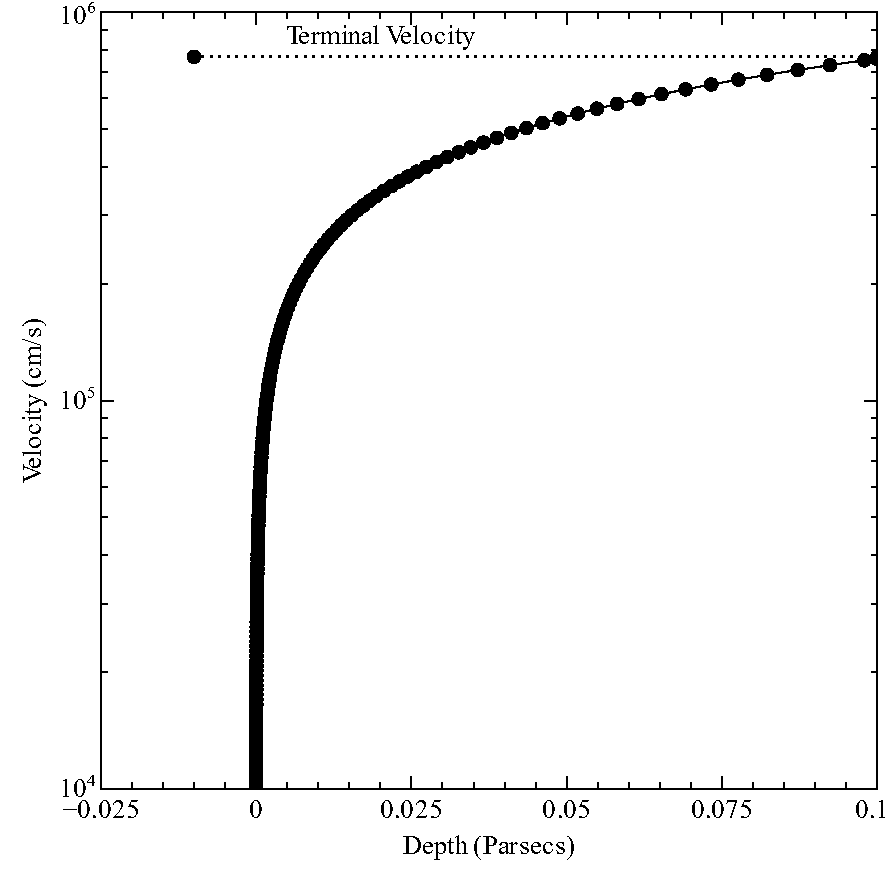
\includegraphics[scale=0.75]{WindVelocityvsDepth}
\caption[Wind velocity vs depth]
{The wind velocity is computed using the input stream shown in
one of the test cases in the last section.  Parameters were chosen to have
a readily computed final velocity.  The velocity at the outer edge of the
slab is within 1 percent of its expected value.}
\label{fig:WindVelocityvsDepth}
\end{figure}

\section{Eddington limit}

The Eddington limit is given by
\begin{equation}
{L_{Edd}} = \frac{{4\pi GcM}}{\kappa } = 1.45 \times
{10^{38}}\frac{M}{{{M_o}}}\frac{{{\kappa _T}}}{\kappa }
\quad [\mathrm{erg~s}^{-1}]
\end{equation}
where $\kappa_T$ is the Thomson opacity and $\kappa$ is the actual gas opacity (generally
several orders of magnitude above Thomson).

\section{Jeans length and mass}

The Jeans length and mass are computed for each zone in the calculation.
The smallest computed Jeans length and mass are saved, and a note is printed
at the end of the calculation if the computed structure is Jeans unstable.

The expression for the Jeans length is
\begin{equation}
{\lambda _J} = {\left( {\frac{{\pi \,k\,T}}{{\mu \,{m_u}G\,\rho }}}
\right)^{1/2}} = 6.257 \times {10^7}{\left( {\frac{T}{{\mu \rho }}}
\right)^{1/2}}
\quad [\mathrm{cm}]
\end{equation}
where $\mu$ is the mean mass per particle of the gas
\begin{equation}
\mu  = \frac{{\sum {{n_i}\,{m_i}} }}{{\sum {{n_i}} }}
\quad [\mathrm{gm}].
\end{equation}

The Jeans mass is then given by
\begin{equation}
{M_J} = \frac{{4\pi }}{3}\;\rho \,{\left( {\frac{{{\lambda _J}}}{2}}
\right)^3}
\quad [\mathrm{gm}]
\end{equation}
where the mass is that of a sphere with radius $\lambda_J /2$.

The minimum Jeans mass is evaluated as the calculation progresses.  The
code will generate a comment if the computed structure is Jeans unstable.

\section{Luminosity Distance}

The luminosity distance DL is given by
\begin{equation}
{D_L} = \left\{ \begin{array}{ccccc}
& \frac{{cz}}{{{H_o}}}\left( {1 + z/2} \right)& {q_o} = 0 \\
& \frac{c}{{{H_o}q_o^2}}\left\{ {{q_o}z + \left( {{q_o} - 1} \right)\left[
{{{\left( {2{q_o}z + 1} \right)}^{1/2}} - 1} \right]} \right\}\quad \,\,
& {q_o} > 0 \\
& \frac{{2c}}{{{H_o}}}\left[ {1 + z - {{\left( {1 + z} \right)}^{1/2}}}
\right]& {q_o} = 1/2 \\
 \end{array} \right.
\quad [\mathrm{cm}]
\end{equation}
For $q_o=1/2$ and $H_o = 70$ km/s/Mpc the luminosity distance is
\begin{equation}
{D_L} = 2.643 \times {10^{26}}\left[ {1 + z - {{\left( {1 + z}
\right)}^{1/2}}} \right]
\quad  [\mathrm{cm}]
\end{equation}
The proper distance $D_P$ is given by ${D_P} = {D_L}\left( {1 + z} \right)$.

\citet{Liske2000} provides expressions giving the cosmological distance and
redshift between any two objects.
\citet{Hogg1999} gives a nice pedagogical
review of distance measures in cosmology.

   %proof 1
\backmatter
\bibliographystyle{plainnat}
\bibliography{../common/bibliography2}

\end{document} 
